\chapter{Avaliação Experimental do Sistema de Controle}\label{cap6}
Após projetar os controladores, fizemos uma avaliação do seu funcionamento, aplicando cada um no sistema real.
\section{Descrição e objetivos experimentais}
Os experimentos descritos neste capítulo tiveram como objetivo, verificar e avaliar o funcionamento do sistema ao ser controlado pelos controladores projetados no capítulo \ref{cap5}. Foram executados 4 experimentos no sistema que funcionam da seguinte forma:
\paragraph{Resposta ao Degrau Unitário} A resposta ao degrau unitário é um experimento onde o sistema recebe uma referência unitária e reage a ela. Com este experimento verificamos se o sistema se mantinha estável ao ser controlado e se ele atendia aos requisitos de tempo de assentamento e máximo sobrevalor definidos quando o controlador foi projetado.
\paragraph{Resposta à escadaria} A resposta à escadaria é um experimento onde o sistema como entrada uma referência que muda de nível em intervalos de tempo, para que possamos verificar se o controlador é capaz de seguir diferentes níveis de referência.

\paragraph{Teste de Robustez à variação paramétrica}

O teste de robustez à mudança de parâmetros serve para determinar se o controlador é capaz de reagir quando algum parâmetro é alterado. Neste experimento, alteramos o peso da bola e verificamos se o sistema era capaz de responder ao degrau unitário.

\paragraph{Teste de Robustez à Perturbação Externa}
  O teste de robustez à perturbação externa mostra se o sistema controlado é capaz de rejeitar perturbações externas ao sistema. Para executar este teste, mediremos a resposta do sistema enquanto obstruímos a saída de ar através dos buracos inferiores do duto do túnel de vento, efetivamente aumentando o fluxo de ar que eleva a bola.

\section{Resultados Experimentais}
Nesta seção serão apresentados os resultados dos experimentos descritos anteriormente.
\subsection{Resultados da Resposta ao degrau unitário}\label{rstep}

Nas figuras desta seção, as linhas pontilhadas indicam os limites de $\pm 5\%$ da referência.

\subsubsection{Modelo $SUB1$}
Nos deparamos com uma grande diferença na figura \ref{fig:steprsub1y}, a resposta simulada (figura \ref{fig:respostadegrausub1c}), atendeu aos requisitos definidos na seção \ref{s:ctrlsub1}, mas o sistema real não atendeu, vemos a comparação na tabela \ref{tb:reqsub1}. Com um tempo de assentamento de 8 segundos, muito maior que o tempo projetado, o sistema real também não atende ao requisito de máximo sobrevalor. Era esperado que o sistema real tivesse problemas de atender os requisitos de tempo de assentamento e máximo sobrevalor porque utilizamos um modelo idealizado para projetar o controlador.

\begin{figure}[htb]
	\centering
	\begin{subfigure}[t]{0.47\textwidth}
		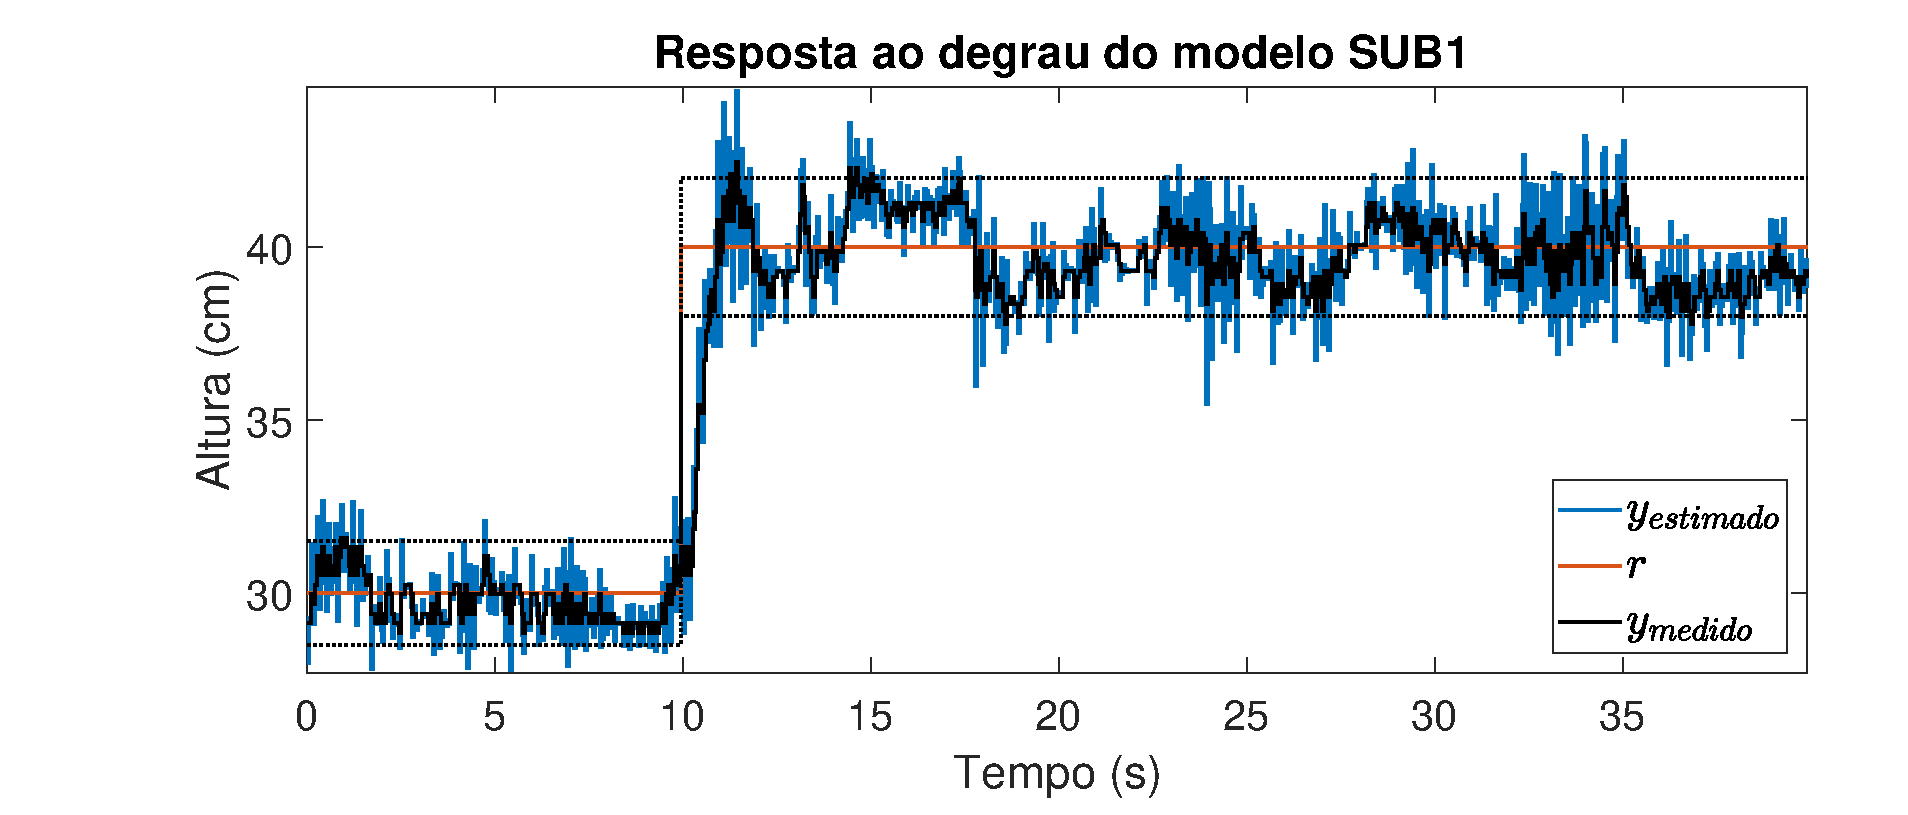
\includegraphics[width=1\linewidth]{steprsub1y}
		\subcaption[$y_{estimado}$ e $y_{medido}$ do modelo $SUB1$]{$y_{estimado}$ e $y_{medido}$ do modelo $SUB1$}
		\label{fig:steprsub1y}
	\end{subfigure}
	~ %add desired spacing between images, e. g. ~, \quad, \qquad, \hfill etc. 
	%(or a blank line to force the subfigure onto a new line)
	~
	\begin{subfigure}[t]{0.47\textwidth}
		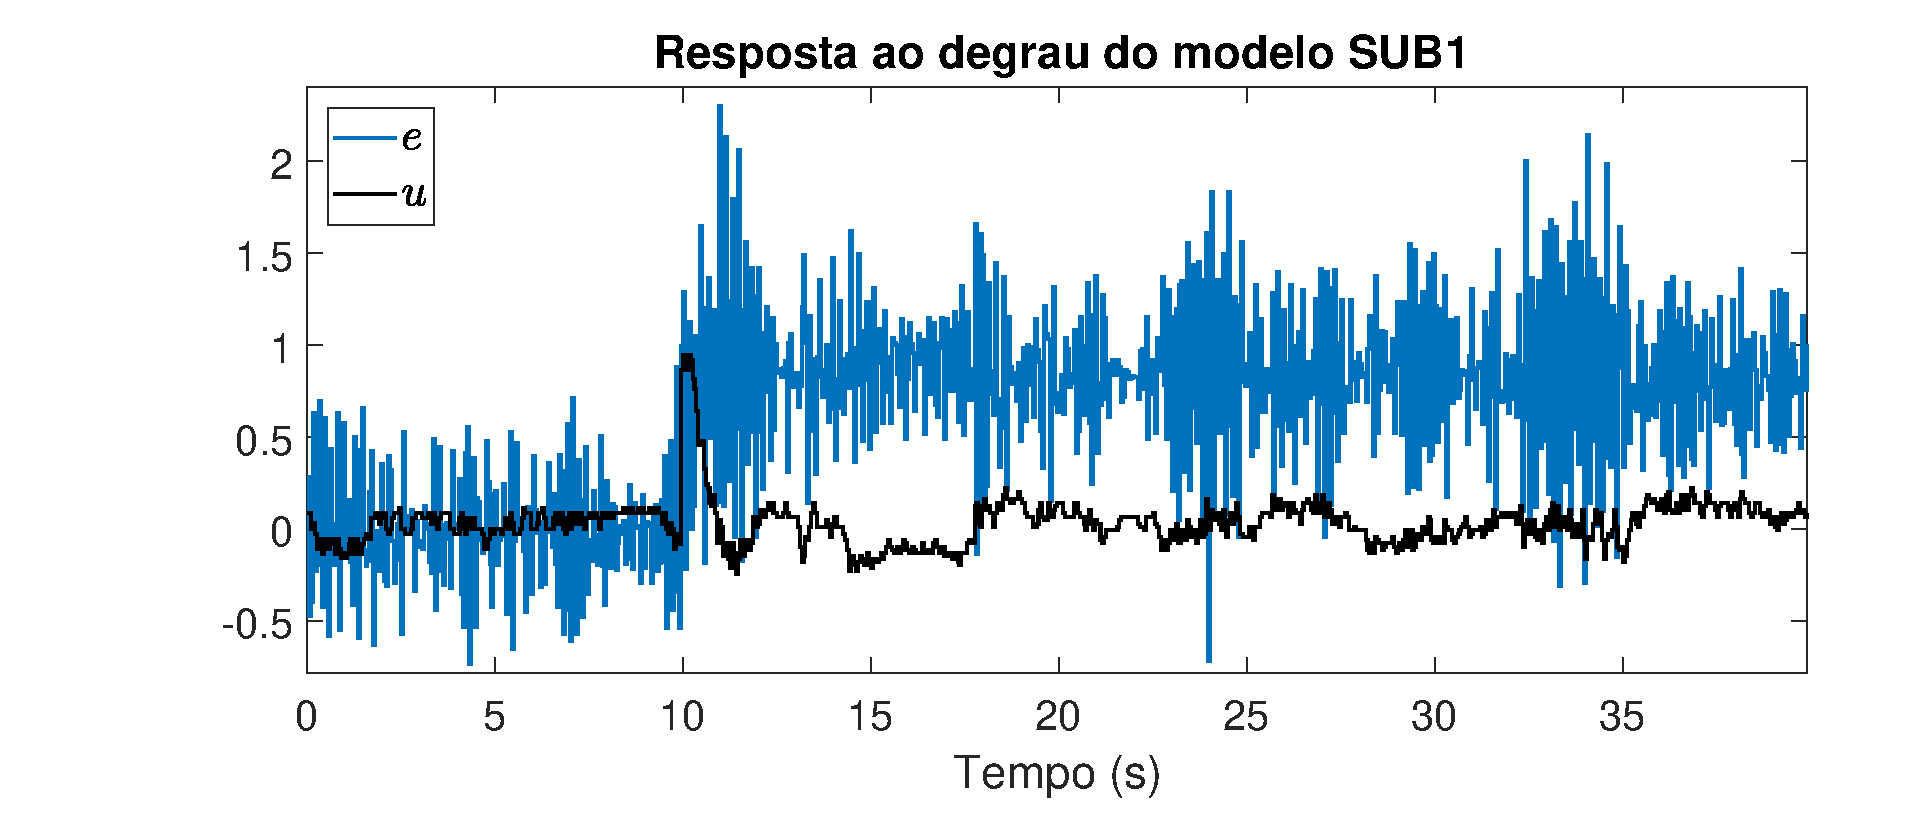
\includegraphics[width=1\linewidth]{steprsub1e}
		\subcaption[erro $e$ e sinal de controle $u$ do controlador $SUB1$]{erro $e$ e sinal de controle $u$ do controlador $SUB1$}
		\label{fig:steprsub1e}
	\end{subfigure}
	~ %add desired spacing between images, e. g. ~, \quad, \qquad, \hfill etc. 
	%(or a blank line to force the subfigure onto a new line)
	
	\caption{Resposta ao degrau do sistema usando o controlador $SUB1$}\label{fig:steprsub1}
\end{figure}

\begin{table}[htb]
	\centering
\begin{tabular}{|c|c|c|}
	\hline 
	Requisitos & Projetado & Real \\ 
	\hline 
	$T_s$ (s) & 0.8 & 8 \\ 
	\hline 
	$ovs\%$ & 0.125\% & 6.1164\% \\ 
	\hline 
\end{tabular} 
\caption{Tabela dos requisitos do sistema $SUB1$}
\label{tb:reqsub1}
\end{table}

\subsubsection{Modelo $ARX1$}

A resposta ao degrau com o controlador do modelo $ARX1$ apresentou os mesmos problemas do modelo $SUB1$ quando aplicado no sistema real: não atendeu aos requisitos de tempo de assentamento e máximo sobrevalor, como vemos na figura \ref{fig:steprarx1y} e na tabela \ref{tb:reqarx1}.
\begin{figure}[htb]
	\centering
	\begin{subfigure}[t]{0.48\textwidth}
		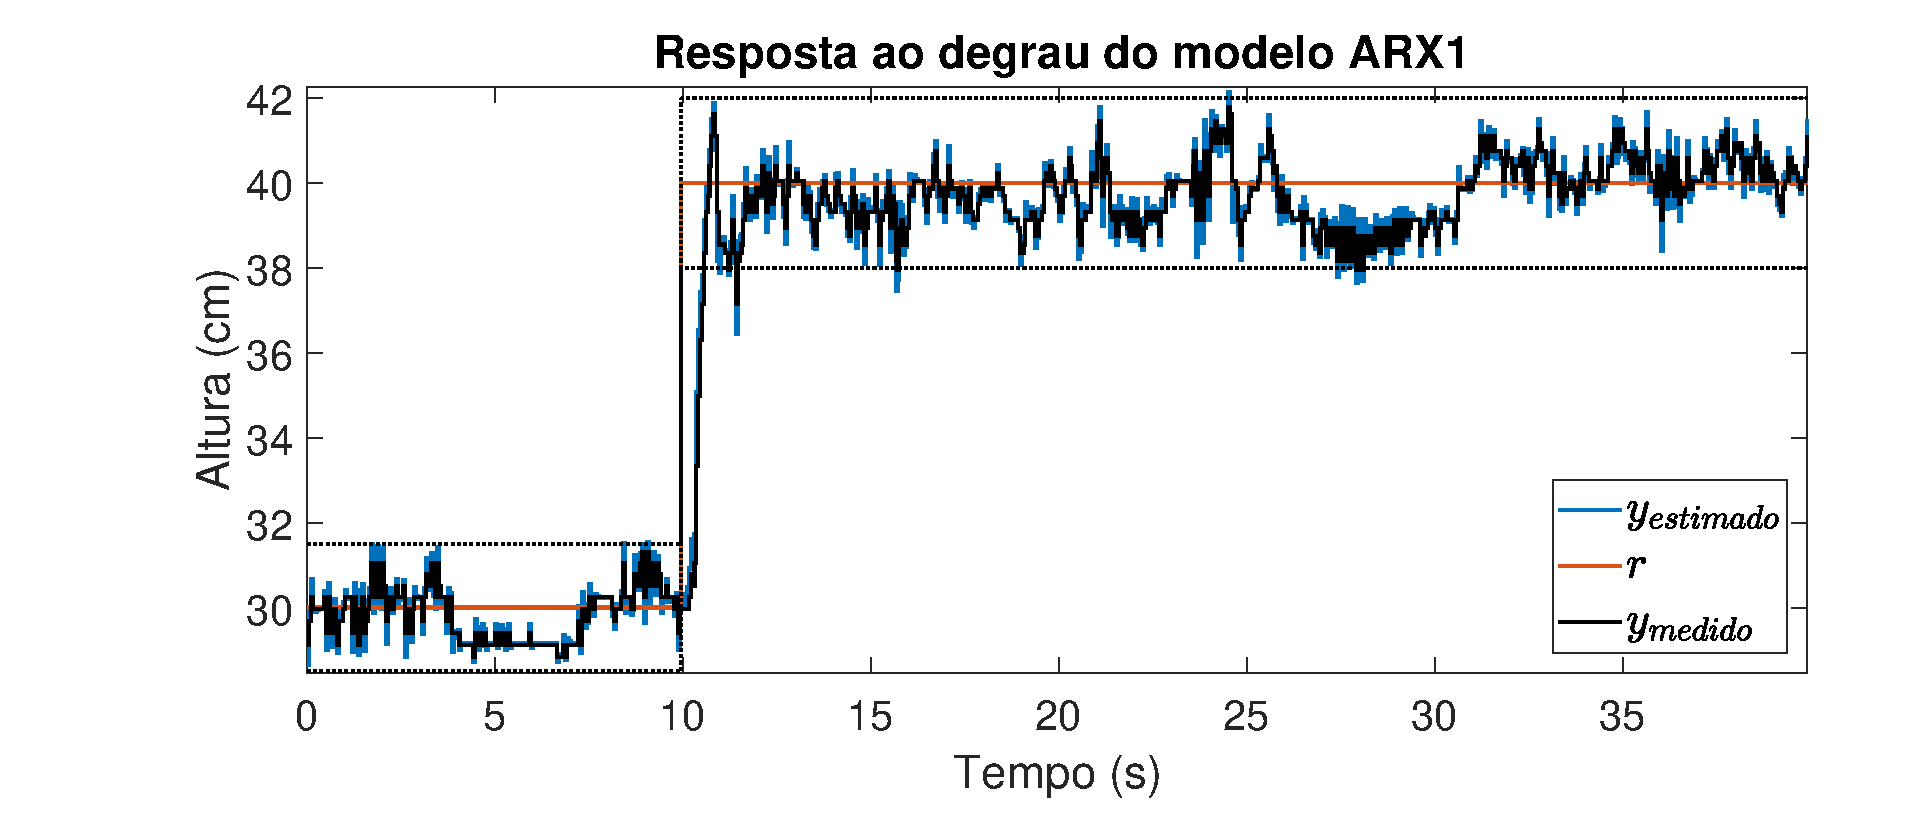
\includegraphics[width=1\linewidth]{steprarx1y}
		\caption[$y_{estimado}$ e $y_{medido}$ do modelo $ARX1$]{$y_{estimado}$ e $y_{medido}$ do modelo $ARX1$}
		\label{fig:steprarx1y}
	\end{subfigure}
	~ %add desired spacing between images, e. g. ~, \quad, \qquad, \hfill etc. 
	%(or a blank line to force the subfigure onto a new line)
	\begin{subfigure}[t]{0.48\textwidth}
		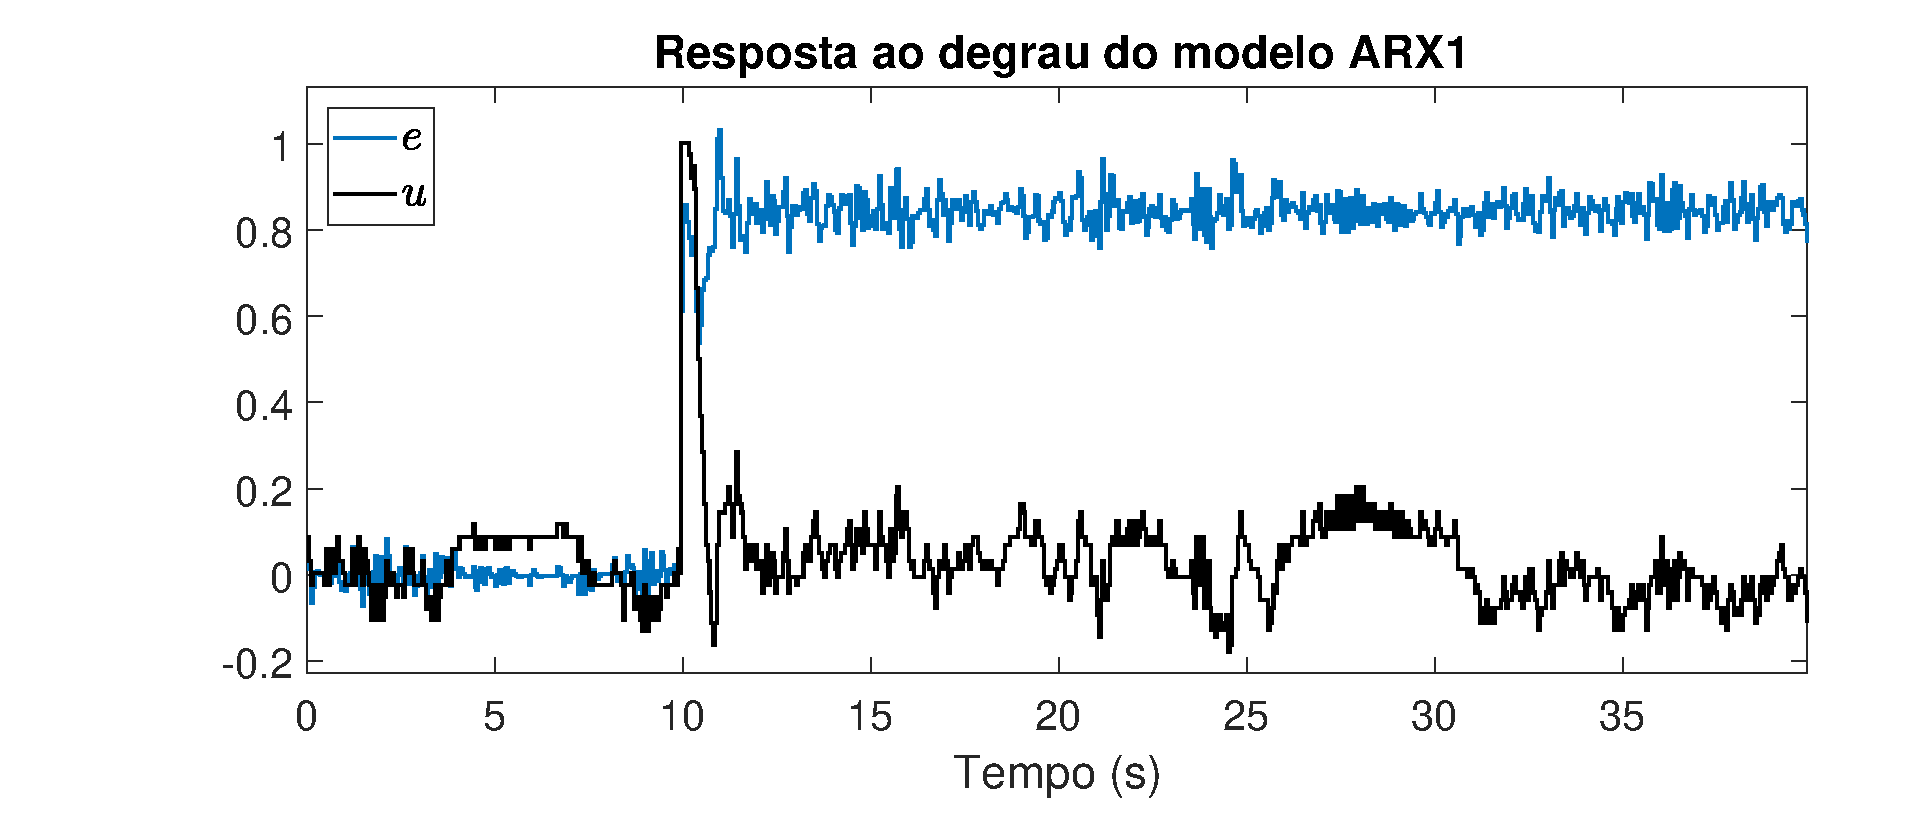
\includegraphics[width=1\linewidth]{steprarx1e}
		\caption[erro $e$ e sinal de controle $u$ do controlador $ARX1$]{erro $e$ e sinal de controle $u$ do controlador $ARX1$}
		\label{fig:steprarx1e}
	\end{subfigure}
	~ %add desired spacing between images, e. g. ~, \quad, \qquad, \hfill etc. 
	%(or a blank line to force the subfigure onto a new line)
	
	\caption{Resposta ao degrau do sistema com o controlador do modelo $ARX1$}\label{fig:steprarx1}
\end{figure}

\begin{table}[htb]
	\centering
	\begin{tabular}{|c|c|c|}
		\hline 
		Requisitos & Projetado & Real \\ 
		\hline 
		$T_s$ (s) & 0.9 & 6 \\ 
		\hline 
		$ovs\%$ & 0.0326\% & 4.4785\% \\ 
		\hline 
	\end{tabular} 
	\caption{Tabela dos requisitos do sistema $ARX1$}
	\label{tb:reqarx1}
\end{table}

\subsubsection{Modelo $ARX2$}
O mesmo problema de não atender aos requisitos apareceu no controlador do modelo $ARX2$, figura \ref{fig:steprarx2y} e na tabela \ref{tb:reqarx2}.
\begin{figure}[htb]
	\centering
	\begin{subfigure}[t]{0.48\textwidth}
		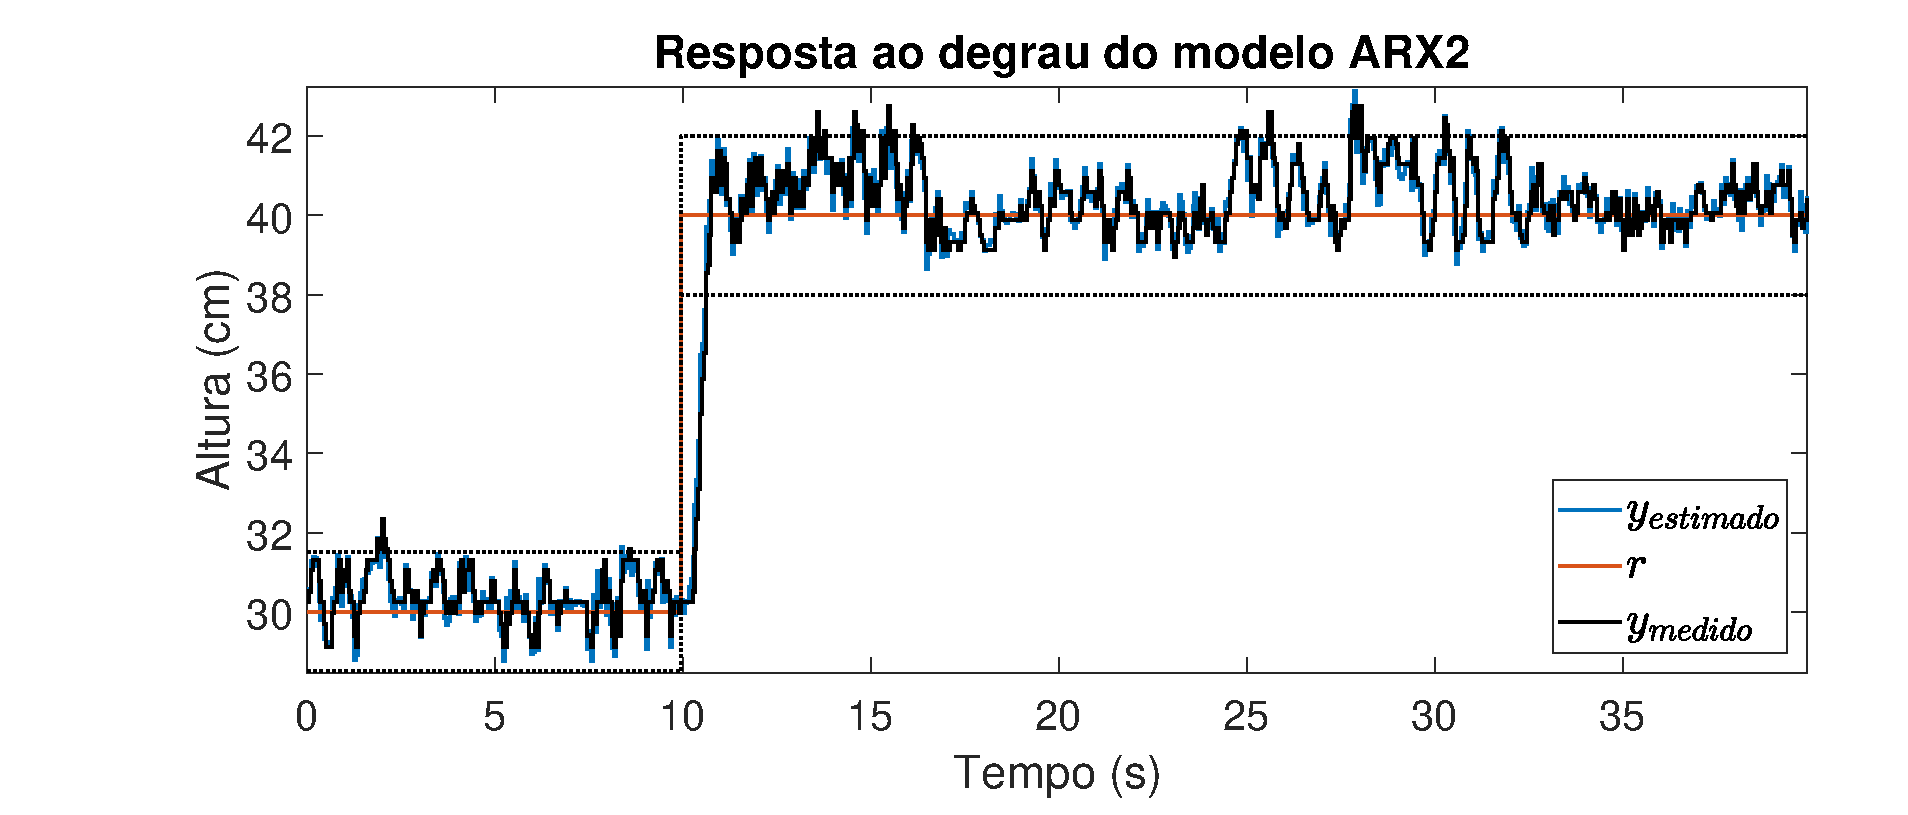
\includegraphics[width=1\linewidth]{steprarx2y}
		\caption[$y_{estimado}$ e $y_{medido}$ do modelo $ARX2$]{$y_{estimado}$ e $y_{medido}$ do modelo $ARX2$}
		\label{fig:steprarx2y}
	\end{subfigure}
	~ %add desired spacing between images, e. g. ~, \quad, \qquad, \hfill etc. 
	%(or a blank line to force the subfigure onto a new line)
	\begin{subfigure}[t]{0.48\textwidth}
		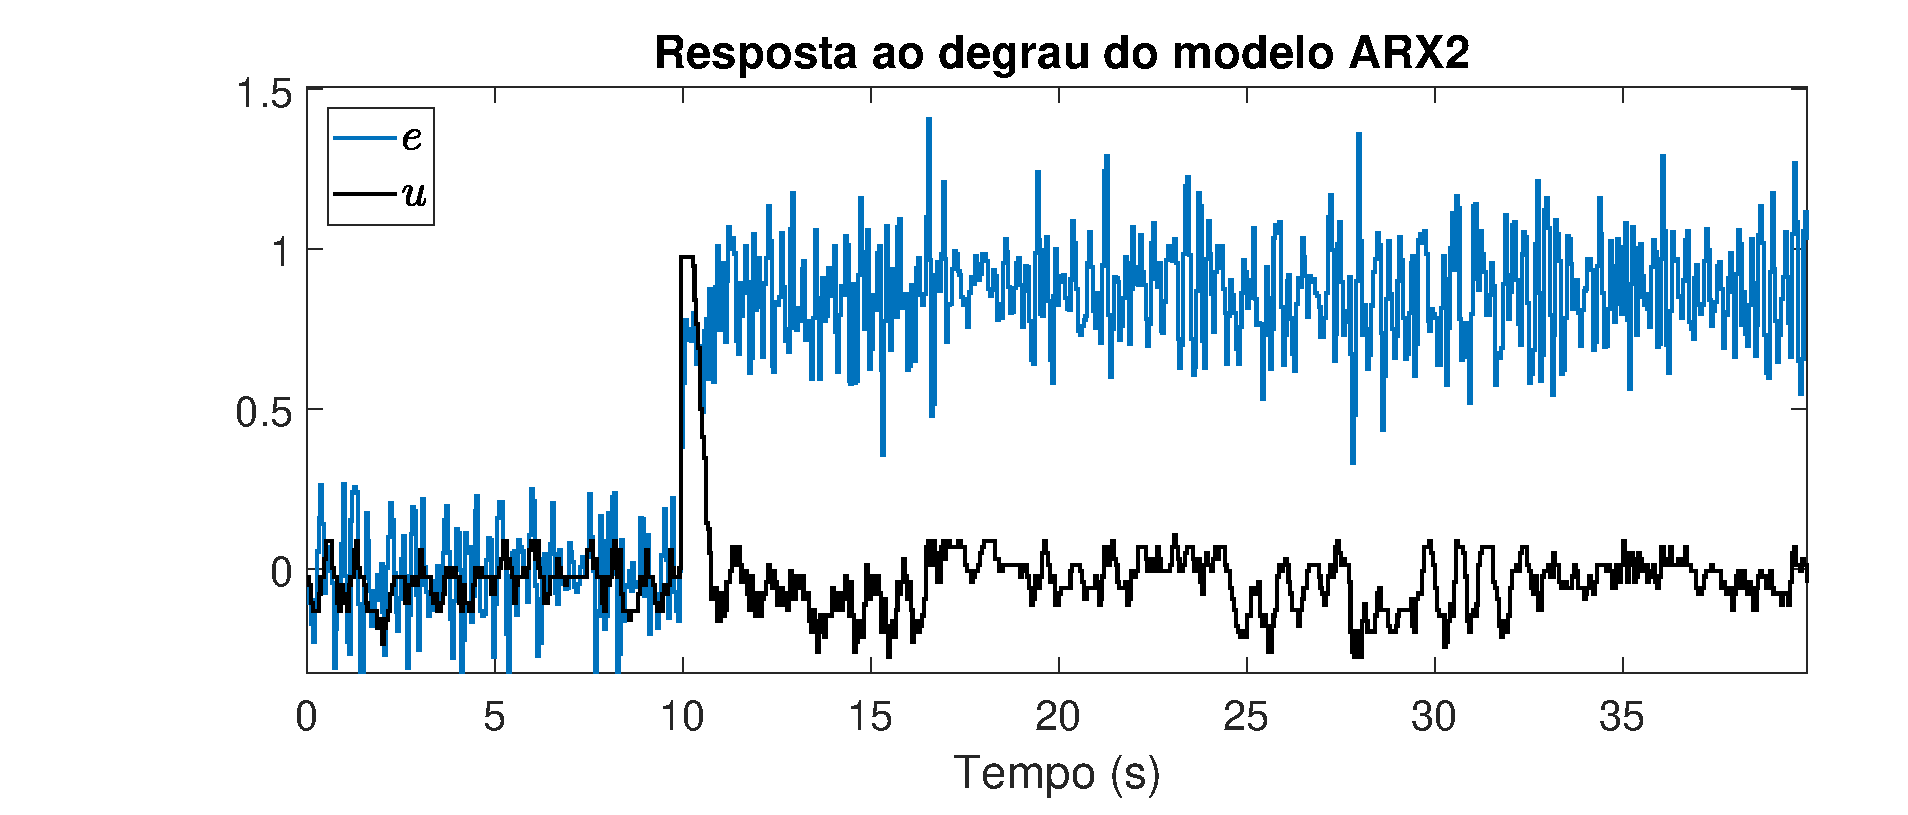
\includegraphics[width=1\linewidth]{steprarx2e}
		\caption[erro $e$ e sinal de controle $u$ do controlador $ARX2$]{erro $e$ e sinal de controle $u$ do controlador $ARX2$}
		\label{fig:steprarx2e}
	\end{subfigure}
	~ %add desired spacing between images, e. g. ~, \quad, \qquad, \hfill etc. 
	%(or a blank line to force the subfigure onto a new line)
	
	\caption{Resposta ao degrau do sistema com o controlador do modelo $ARX2$}\label{fig:steprarx2}
\end{figure}

\begin{table}[htb]
	\centering
	\begin{tabular}{|c|c|c|}
		\hline 
		Requisitos & Projetado & Real \\ 
		\hline 
		$T_s$ (s) & 1.3 & 6 \\ 
		\hline 
		$ovs\%$ & 0.1487\% & 6.9156\% \\ 
		\hline 
	\end{tabular} 
	\caption{Tabela dos requisitos do sistema $SUB1$}
	\label{tb:reqarx2}
\end{table}

\subsubsection{Modelo $ARXsim$}

Tentamos aplicar o controlador do modelo $ARXsim$ no sistema real, mas o ganho do controlador foi muito alto, o que saturou o sinal de controle do motor. Portanto, simulamos esse modelo. Vemos a sua resposta ao degrau na figura \ref{fig:stepsarxsimy} e observamos que o sistema é completamente diferente do sistema real, o estimador de estados não está estimando a posição corretamente apesar de ter sido projetado de forma correta. Entretanto, mesmo com o estimador errado, a saída do sistema chega perto do degrau unitário.

\begin{figure}[htb]
	\centering
	\begin{subfigure}[t]{0.48\textwidth}
		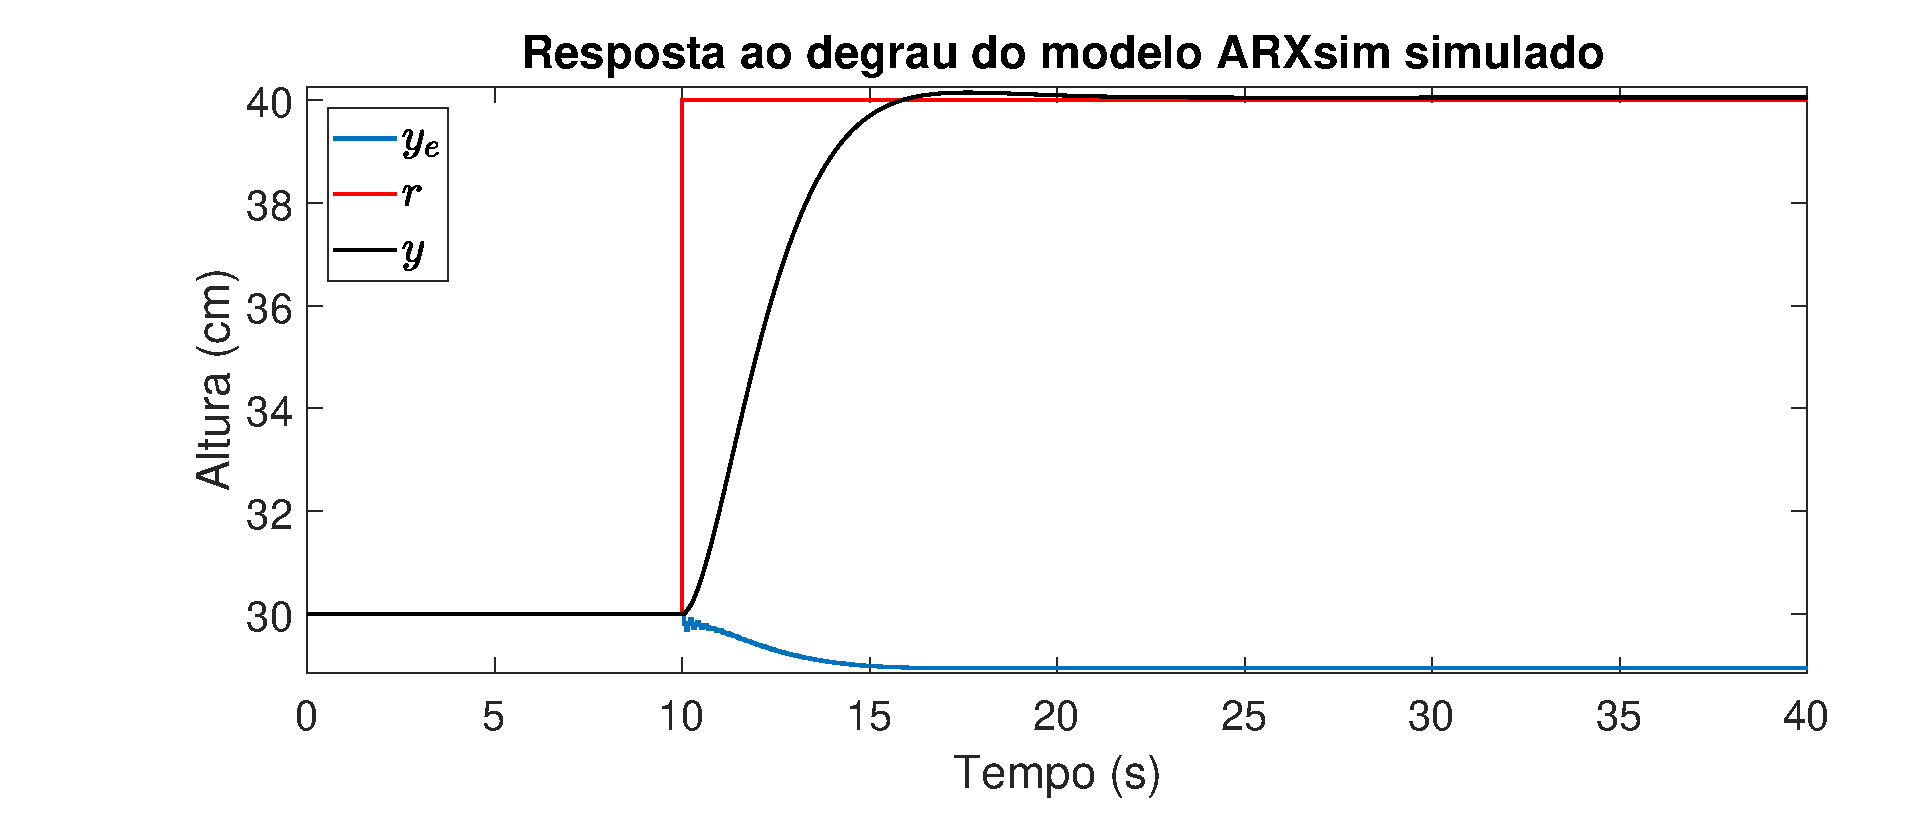
\includegraphics[width=1\linewidth]{pasta1_figuras/stepsarxsimy}
		\caption[$y_{estimado}$ e $y_{medido}$ do modelo $ARX2$]{$y_{estimado}$ e $y_{medido}$ do modelo $ARXsim$}
		\label{fig:stepsarxsimy}
	\end{subfigure}
	~ %add desired spacing between images, e. g. ~, \quad, \qquad, \hfill etc. 
	%(or a blank line to force the subfigure onto a new line)
	\begin{subfigure}[t]{0.48\textwidth}
		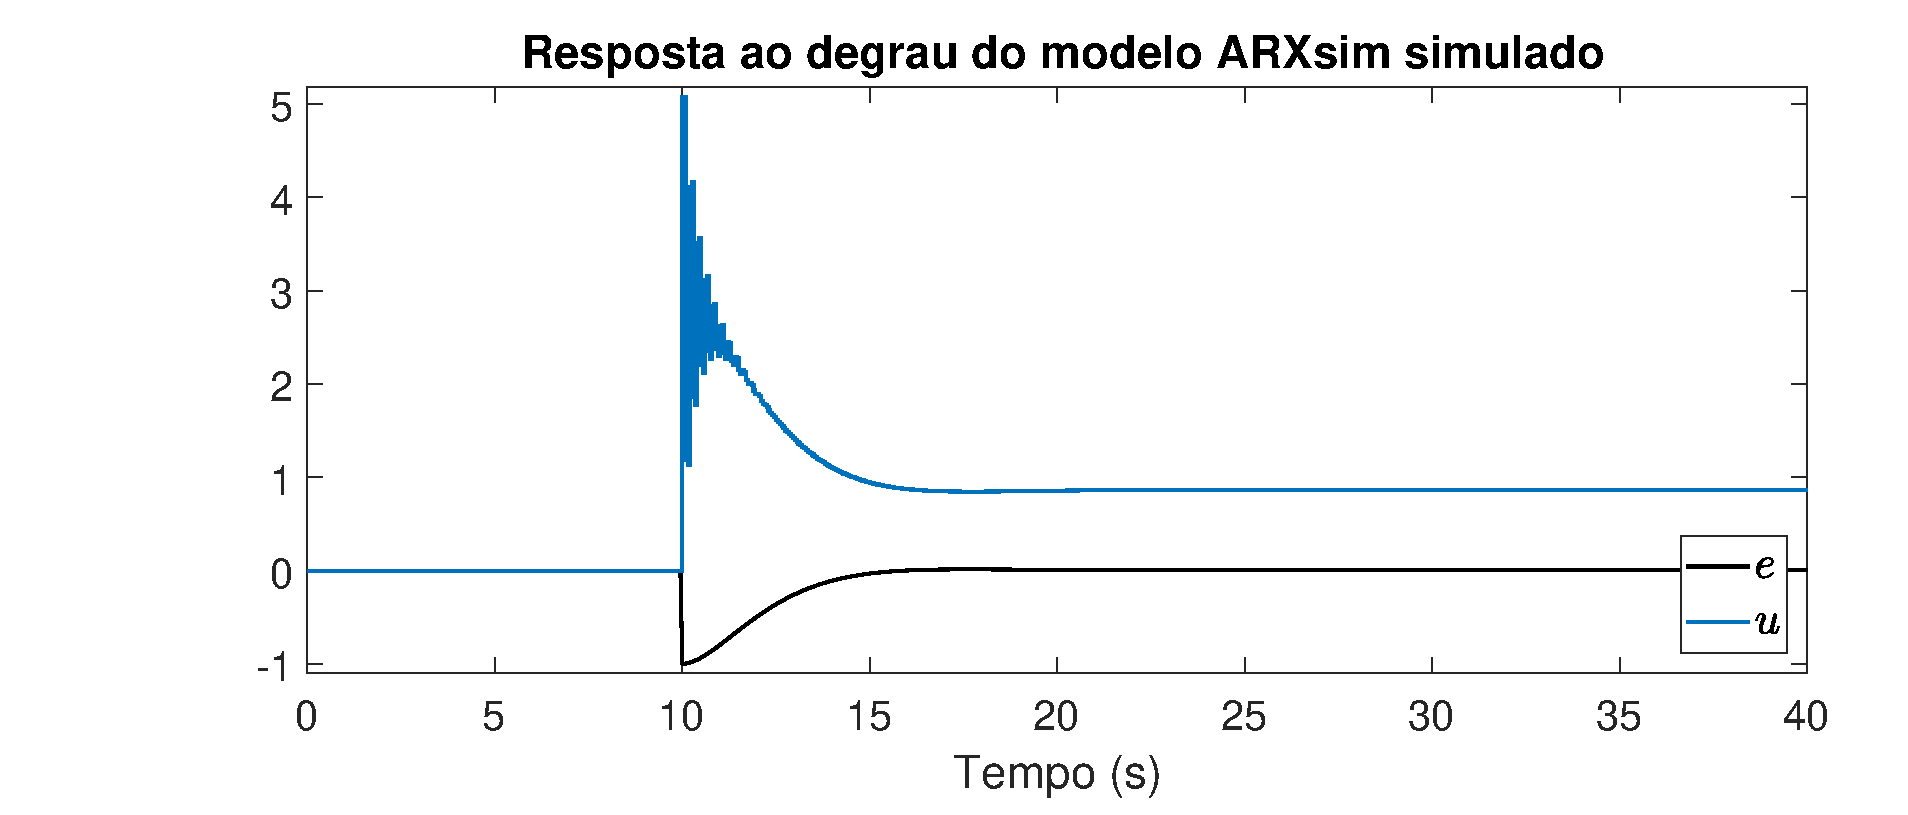
\includegraphics[width=1\linewidth]{pasta1_figuras/stepsarxsime}
		\caption[erro $e$ e sinal de controle $u$ do controlador $ARX2$]{erro $e$ e sinal de controle $u$ do controlador $ARXsim$}
		\label{fig:stepsarxsime}
	\end{subfigure}
	~ %add desired spacing between images, e. g. ~, \quad, \qquad, \hfill etc. 
	%(or a blank line to force the subfigure onto a new line)
	
	\caption{Resposta ao degrau do sistema com o controlador do modelo $ARXsim$}\label{fig:stepsarxsim}
\end{figure}

\subsubsection{ISE da resposta ao degrau dos modelos simulada}

O ISE é um índice de desempenho de sistema que quantifica o desempenho de um sistema para respostas rápidas pela equação \eqref{eq:ise}. Vemos na figura \ref{fig:ise}, um gráfico com os 4 modelos identificados, $SUB1$, $ARX1$, $ARX2$ e $ARXsim$, com o ISE calculado para sua resposta ao degrau de -1 à 1. Com esse gráfico, vemos que o controlador que mais minimizou o erro foi o do modelo $ARX1$ e o que menos minimizou o erro, o do modelo $ARXsim$, o que era de se esperar dado que o modelo $ARXsim$ não é um modelo adequado. 

\begin{equation}\label{eq:ise}
ISE=\int e^2 dt
\end{equation}

\begin{figure}[htb]
	\centering
	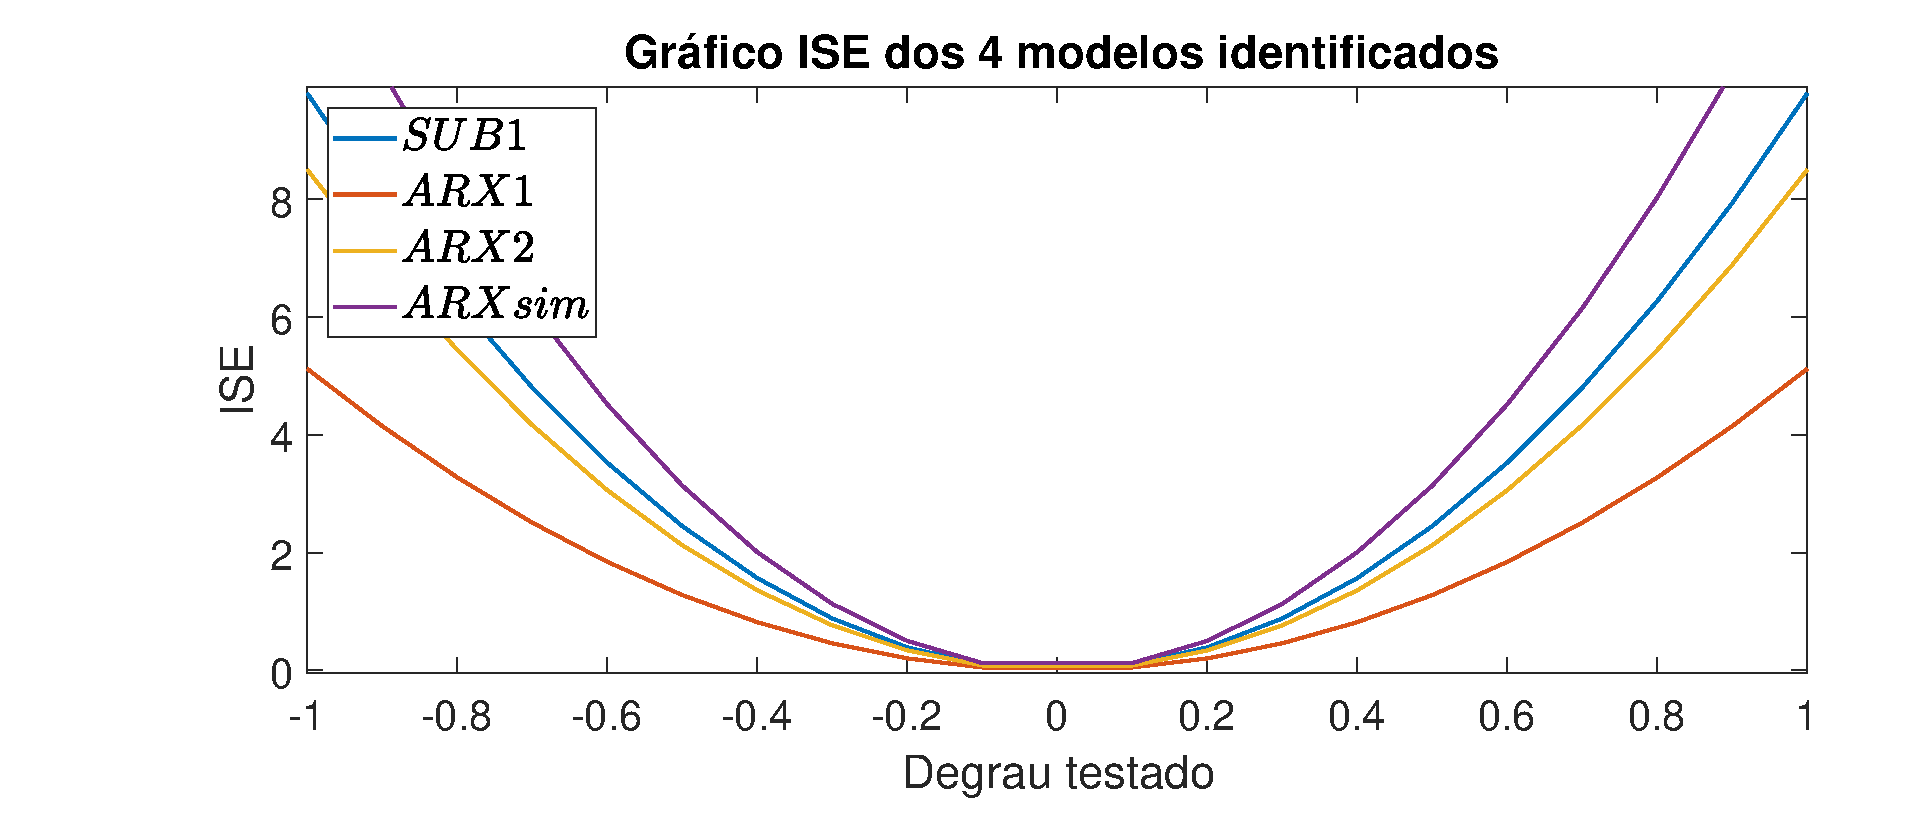
\includegraphics[width=1\linewidth]{pasta1_figuras/ise}
	\caption[Gráfico ISE dos 4 modelos estimados]{Gráfico ISE dos 4 modelos estimados}
	\label{fig:ise}
\end{figure}

\subsubsection{Comparação dos modelos}

Na tabela \ref{tb:requisitosise}, mostramos os requisitos de resposta ao degrau definidos. Vemos que no sistema real, nenhum dos modelos foi capaz de atender aos requisitos de sobrevalor e de tempo de assentamento, e o índice ISE foi muito superior ao índice calculado para o modelo simulado.

\begin{table}[htb]
	\centering
	\begin{tabular}{l|r|r|r|r|r|r|}
		\cline{2-7}
		& \multicolumn{3}{c|}{\textbf{Teste}}                                                                                                        & \multicolumn{3}{c|}{\textbf{Modelo Simulado}}                                                                                              \\ \hline
		\multicolumn{1}{|l|}{\textit{\textbf{Modelos}}} & \multicolumn{1}{l|}{\textit{\textbf{$t_s$ (s)}}} & \multicolumn{1}{l|}{\textit{\textbf{OVS}}} & \multicolumn{1}{l|}{\textit{\textbf{ISE}}} & \multicolumn{1}{l|}{\textit{\textbf{$t_s$ (s)}}} & \multicolumn{1}{l|}{\textit{\textbf{OVS}}} & \multicolumn{1}{l|}{\textit{\textbf{ISE}}} \\ \hline
		\multicolumn{1}{|l|}{$SUB1$}                    & 8                                                & 6.125\%                                    & 14.2801                                    & 0.8                                              & 0.125\%                                    & 9.8033                                     \\ \hline
		\multicolumn{1}{|l|}{$ARX1$}                    & 6                                                & 4.4785\%                                   & 13.0572                                    & 0.9                                              & 0.0326\%                                   & 5.1225                                     \\ \hline
		\multicolumn{1}{|l|}{$ARX2$}                    & 6                                                & 6.9156\%                                   & 15.2428                                    & 1.3                                              & 0.1487\%                                   & 8.5043                                     \\ \hline
		\multicolumn{1}{|l|}{$ARXsim$}                  & 6                                                & 0\%                                        & 8.5043                                     & 1.3                                              & 0.14\%                                     & 8.1588                                     \\ \hline
	\end{tabular}
\caption{Tabela de comparação dos requisitos de controle dos modelos e índice ISE}
\label{tb:requisitosise}
\end{table}

\subsection{Resultados da Resposta à Escadaria}\label{rstair}

\subsubsection{Modelo $SUB1$}
Testamos a resposta à escadaria do controlador do modelo $SUB1$ e constatamos que ele foi capaz de seguir a referência (figura \ref{fig:stairrsub1y}).

\begin{figure}[htb]
	\centering
	\begin{subfigure}[t]{0.48\textwidth}
		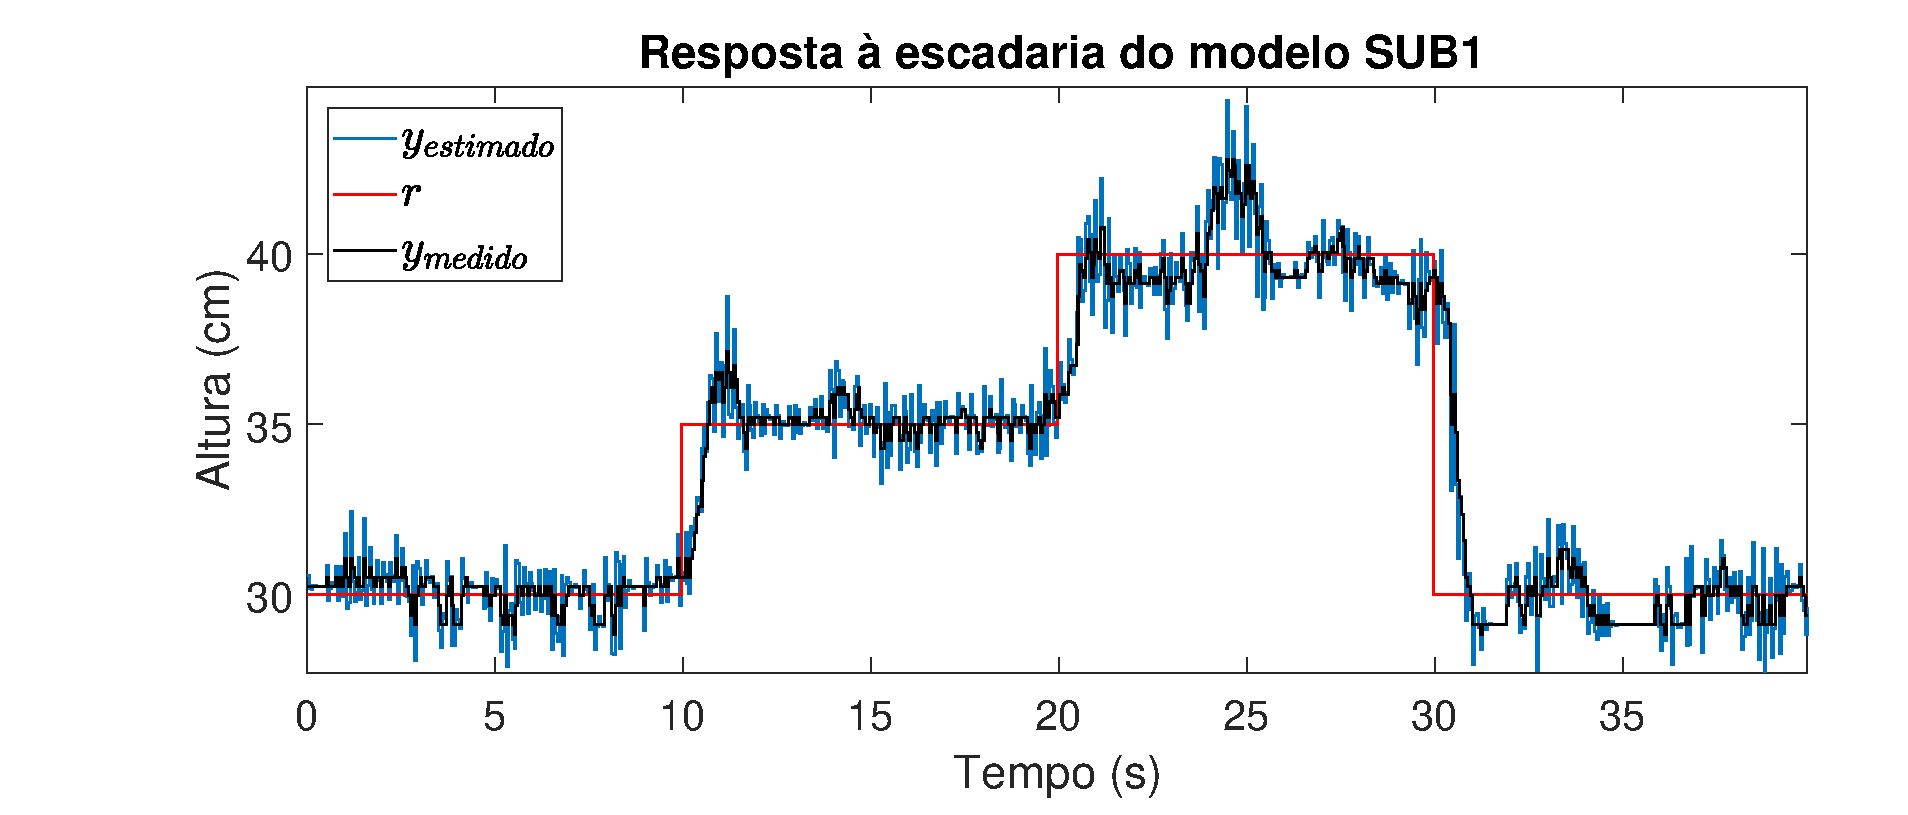
\includegraphics[width=1\linewidth]{stairrsub1y}
		\caption[$y_{estimado}$ e $y_{medido}$ do modelo $SUB1$]{$y_{estimado}$ e $y_{medido}$ do modelo $SUB1$}
		\label{fig:stairrsub1y}
	\end{subfigure}
	~ %add desired spacing between images, e. g. ~, \quad, \qquad, \hfill etc. 
	%(or a blank line to force the subfigure onto a new line)
	\begin{subfigure}[t]{0.48\textwidth}
		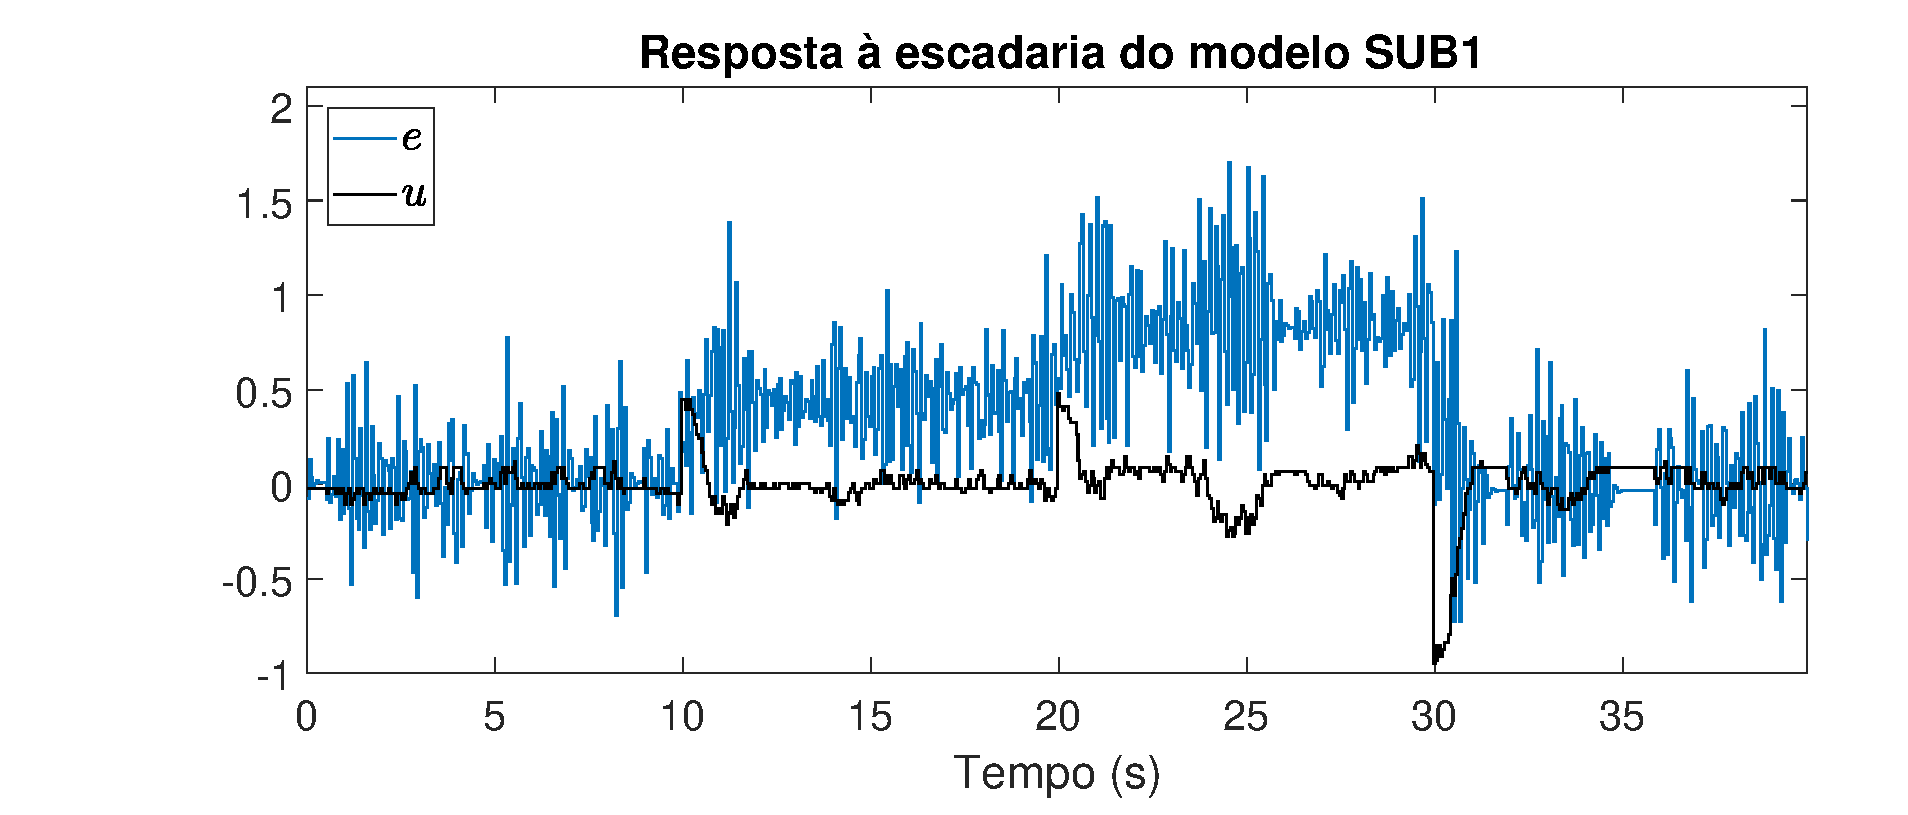
\includegraphics[width=1\linewidth]{stairrsub1e}
		\caption[erro $e$ e sinal de controle $u$ do controlador $SUB1$]{erro $e$ e sinal de controle $u$ do controlador $SUB1$}
		\label{fig:stairrsub1e}
	\end{subfigure}
	~ %add desired spacing between images, e. g. ~, \quad, \qquad, \hfill etc. 
	%(or a blank line to force the subfigure onto a new line)
	
	\caption{Resposta à escadaria do sistema com o controlador do modelo $SUB1$}\label{fig:stairrsub1}
\end{figure}

\subsubsection{Modelo $ARX1$}
A resposta à escadaria do sistema real controlado por $ARX1$ nos mostra que ele foi capaz de seguir a referência (figura \ref{fig:stairrarx1y}).

\begin{figure}[htb]
	\centering
	\begin{subfigure}[t]{0.48\textwidth}
		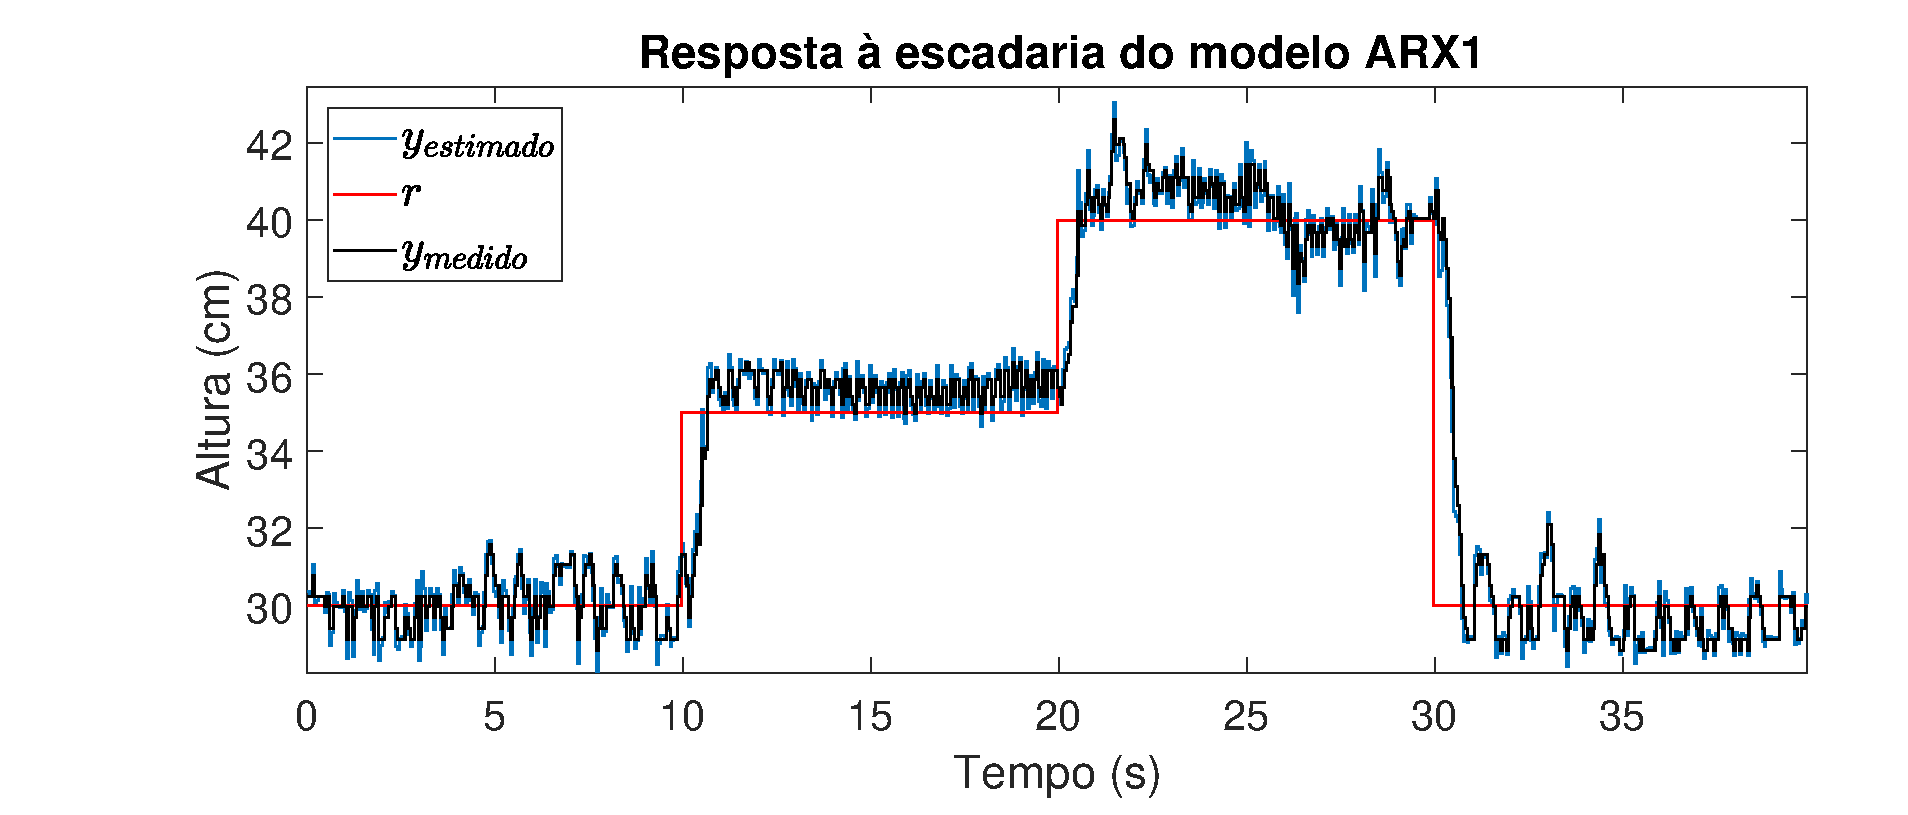
\includegraphics[width=1\linewidth]{stairrarx1y}
		\caption[$y_{estimado}$ e $y_{medido}$ do modelo $ARX1$]{$y_{estimado}$ e $y_{medido}$ do modelo $ARX1$}
		\label{fig:stairrarx1y}
	\end{subfigure}
	~ %add desired spacing between images, e. g. ~, \quad, \qquad, \hfill etc. 
	%(or a blank line to force the subfigure onto a new line)
	\begin{subfigure}[t]{0.48\textwidth}
		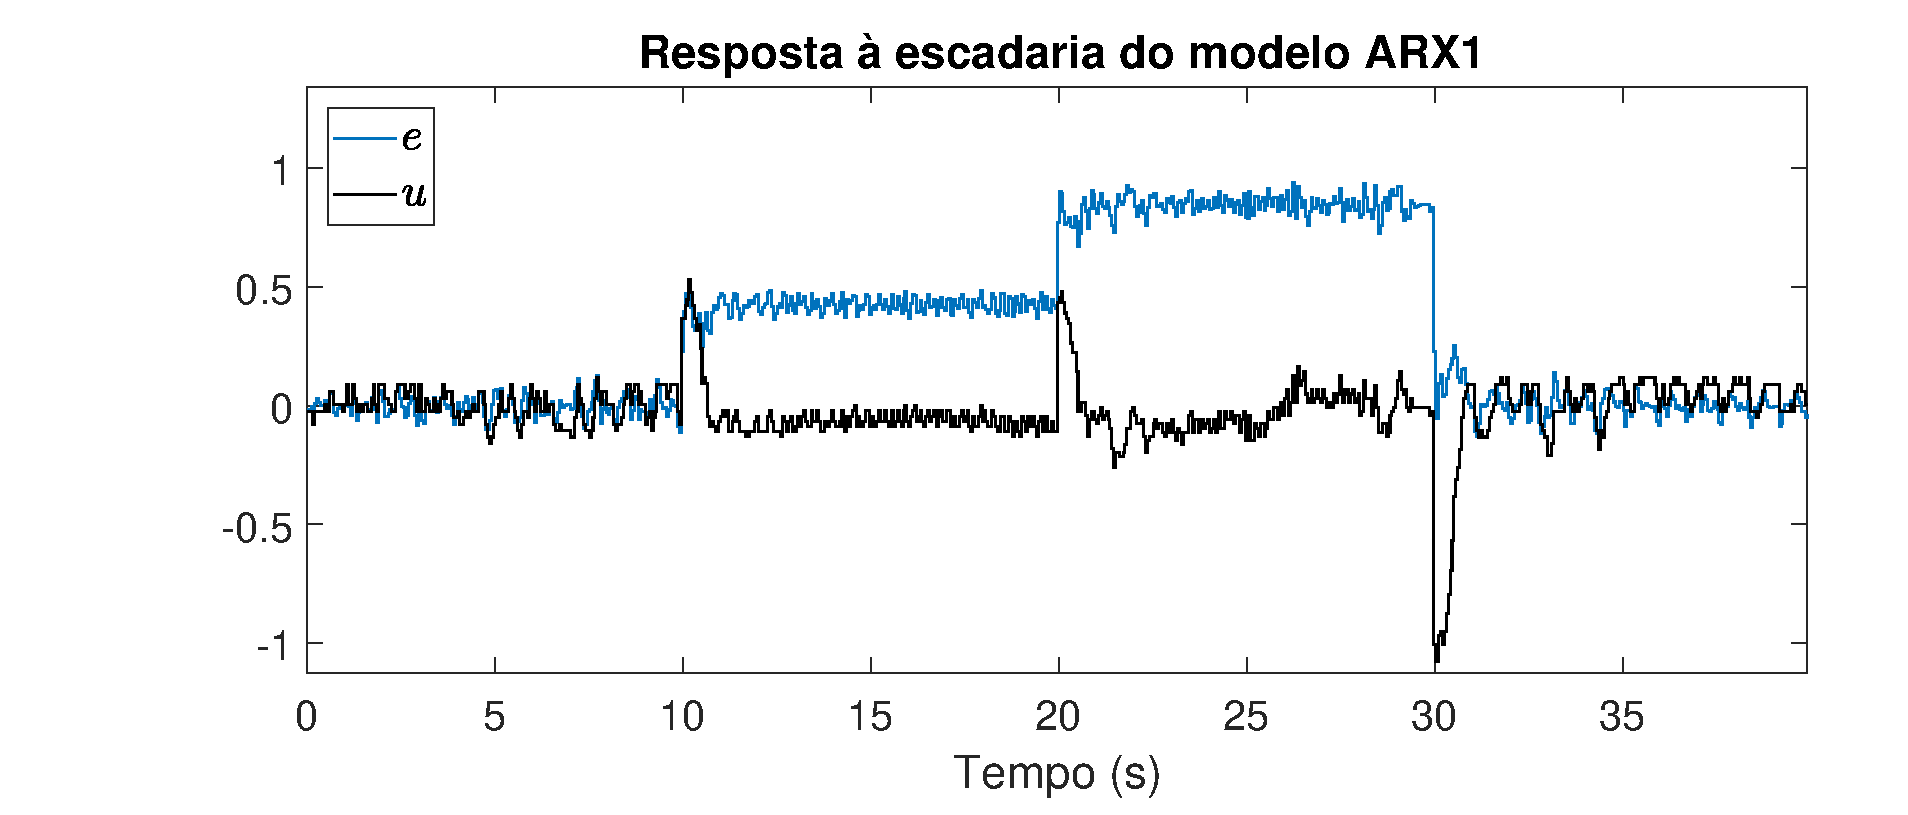
\includegraphics[width=1\linewidth]{stairrarx1e}
		\caption[erro $e$ e sinal de controle $u$ do controlador $ARX1$]{erro $e$ e sinal de controle $u$ do controlador $ARX1$}
		\label{fig:stairrarx1e}
	\end{subfigure}
	~ %add desired spacing between images, e. g. ~, \quad, \qquad, \hfill etc. 
	%(or a blank line to force the subfigure onto a new line)
	
	\caption{Resposta à escadaria do sistema com o controlador do modelo $ARX1$}\label{fig:stairrarx1}
\end{figure}

\subsubsection{Modelo $ARX2$}
A resposta à escadaria do modelo $ARX2$ também foi capaz de seguir a referência (figura \ref{fig:stairrarx2y}).

\begin{figure}[htb]
	\centering
	\begin{subfigure}[t]{0.48\textwidth}
		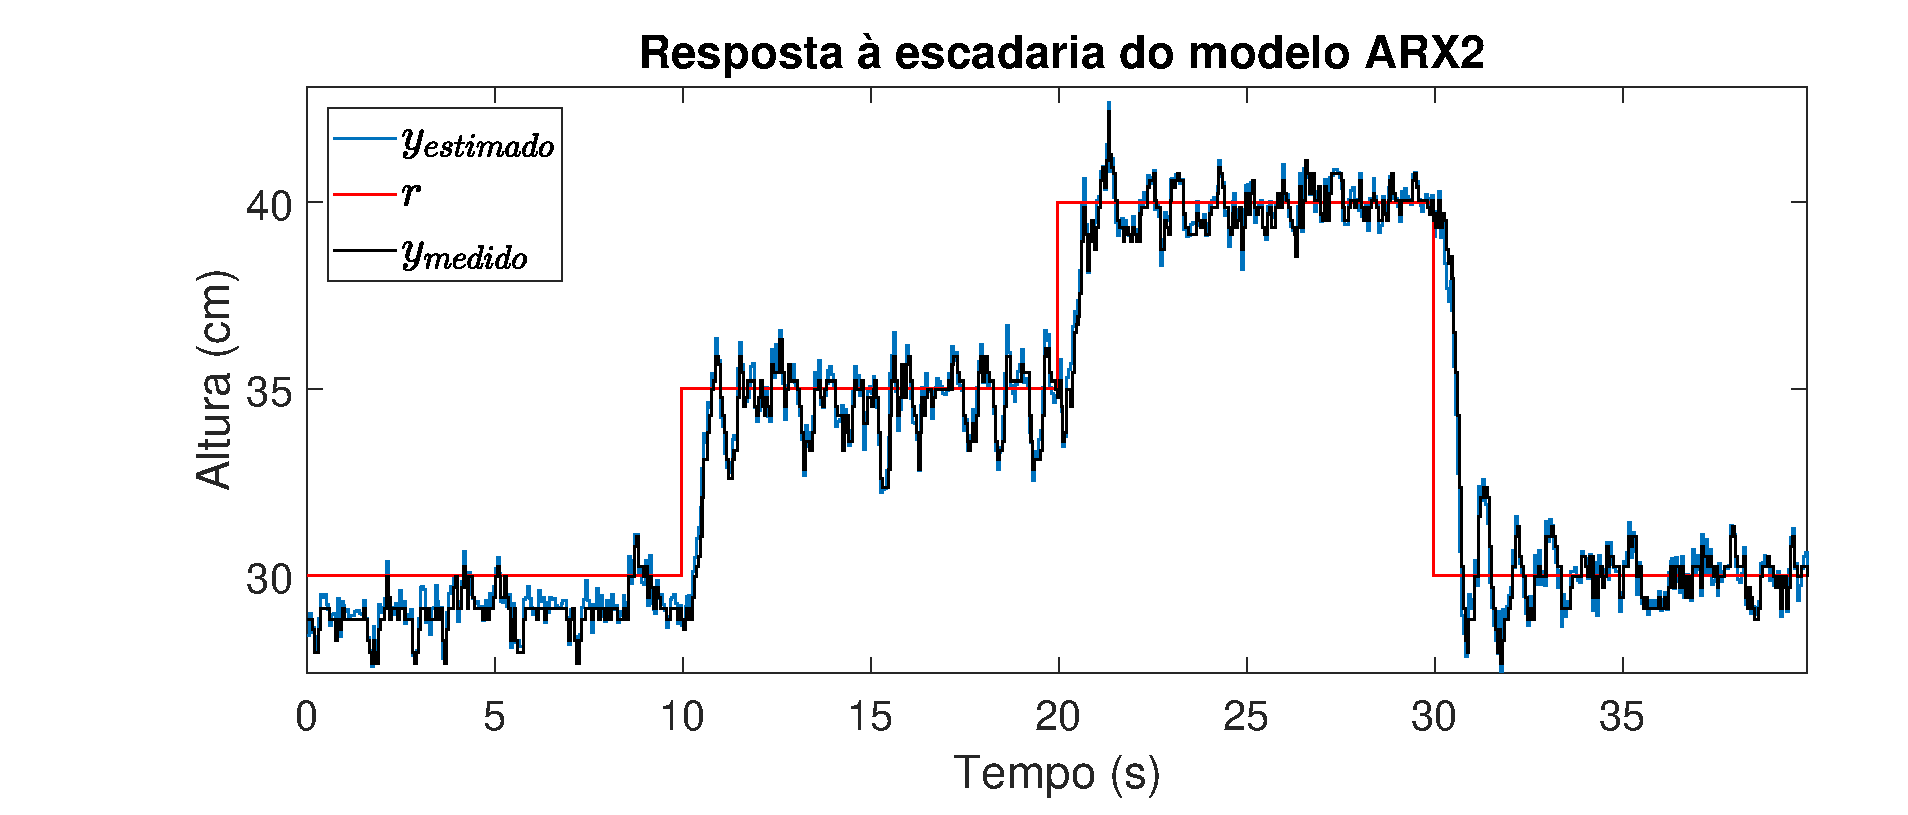
\includegraphics[width=1\linewidth]{stairrarx2y}
		\caption[$y_{estimado}$ e $y_{medido}$ do modelo $ARX2$]{$y_{estimado}$ e $y_{medido}$ do modelo $ARX2$}
		\label{fig:stairrarx2y}
	\end{subfigure}
	~ %add desired spacing between images, e. g. ~, \quad, \qquad, \hfill etc. 
	%(or a blank line to force the subfigure onto a new line)
	\begin{subfigure}[t]{0.48\textwidth}
		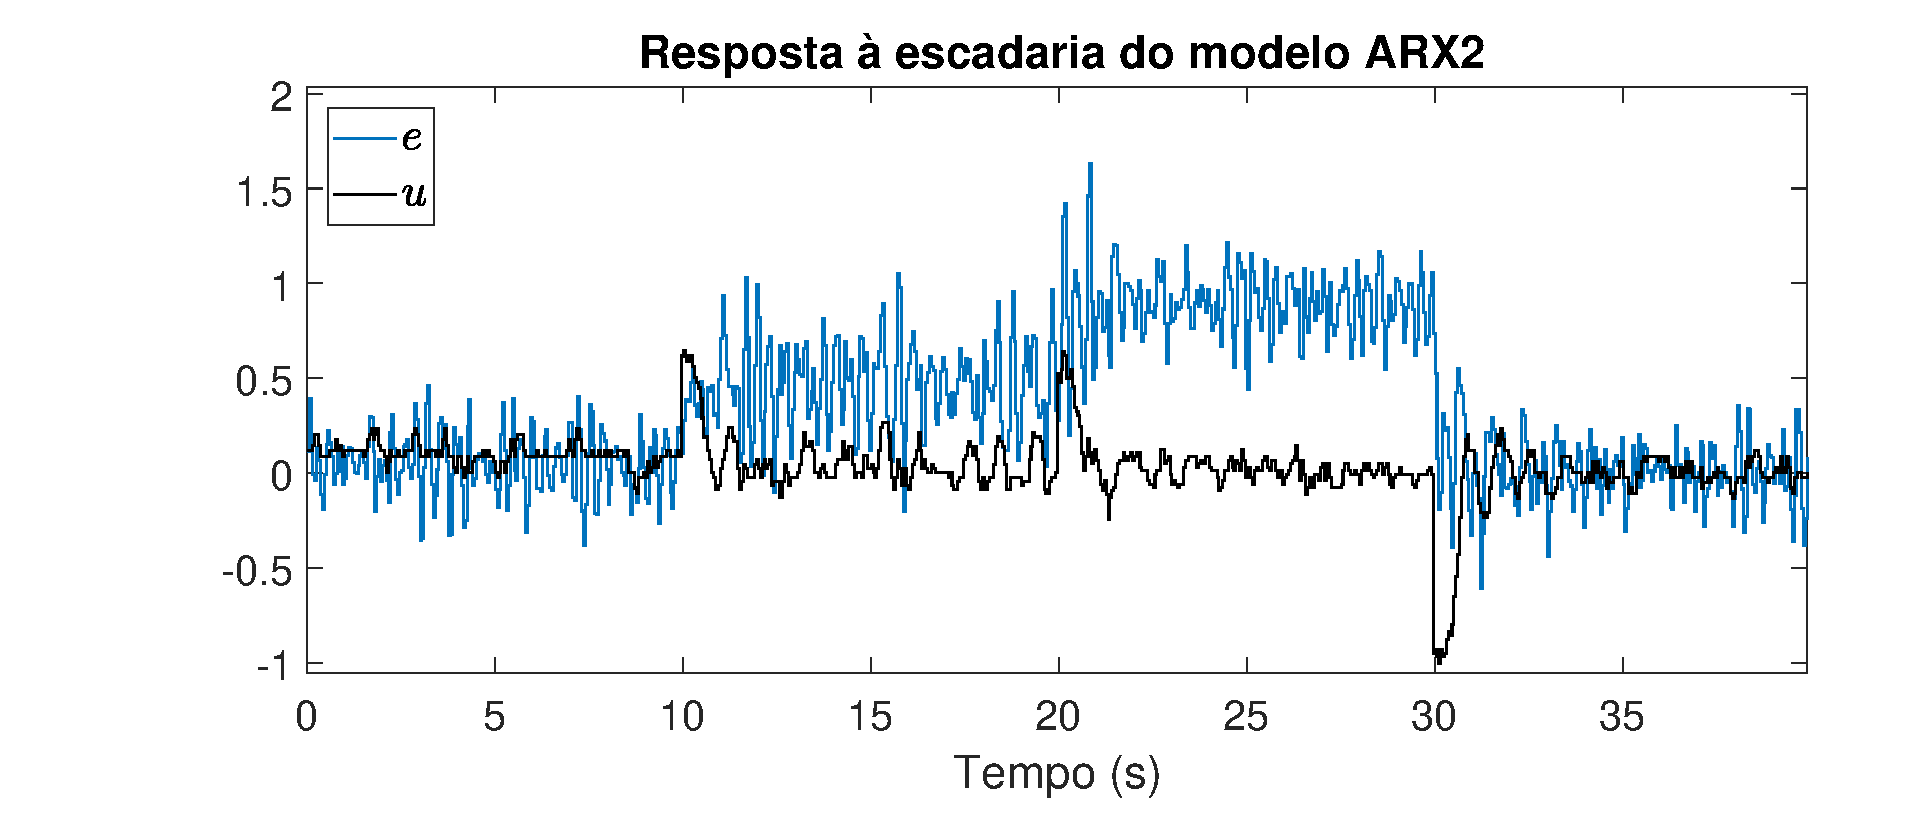
\includegraphics[width=1\linewidth]{stairrarx2e}
		\caption[erro $e$ e sinal de controle $u$ do controlador $ARX2$]{erro $e$ e sinal de controle $u$ do controlador $ARX2$}
		\label{fig:stairrarx2e}
	\end{subfigure}
	~ %add desired spacing between images, e. g. ~, \quad, \qquad, \hfill etc. 
	%(or a blank line to force the subfigure onto a new line)
	
	\caption{Resposta à escadaria do sistema com o controlador do modelo $ARX2$}\label{fig:stairrarx2}
\end{figure}

\subsubsection{Modelo $ARXsim$}

Testamos o controlador do modelo $ARXsim$ para um sinal de referência do tipo escadaria. Vemos na figura \ref{fig:stairsarxsimy}, que o modelo seguiu a referência.

\begin{figure}[htb]
	\centering
	\begin{subfigure}[t]{0.48\textwidth}
		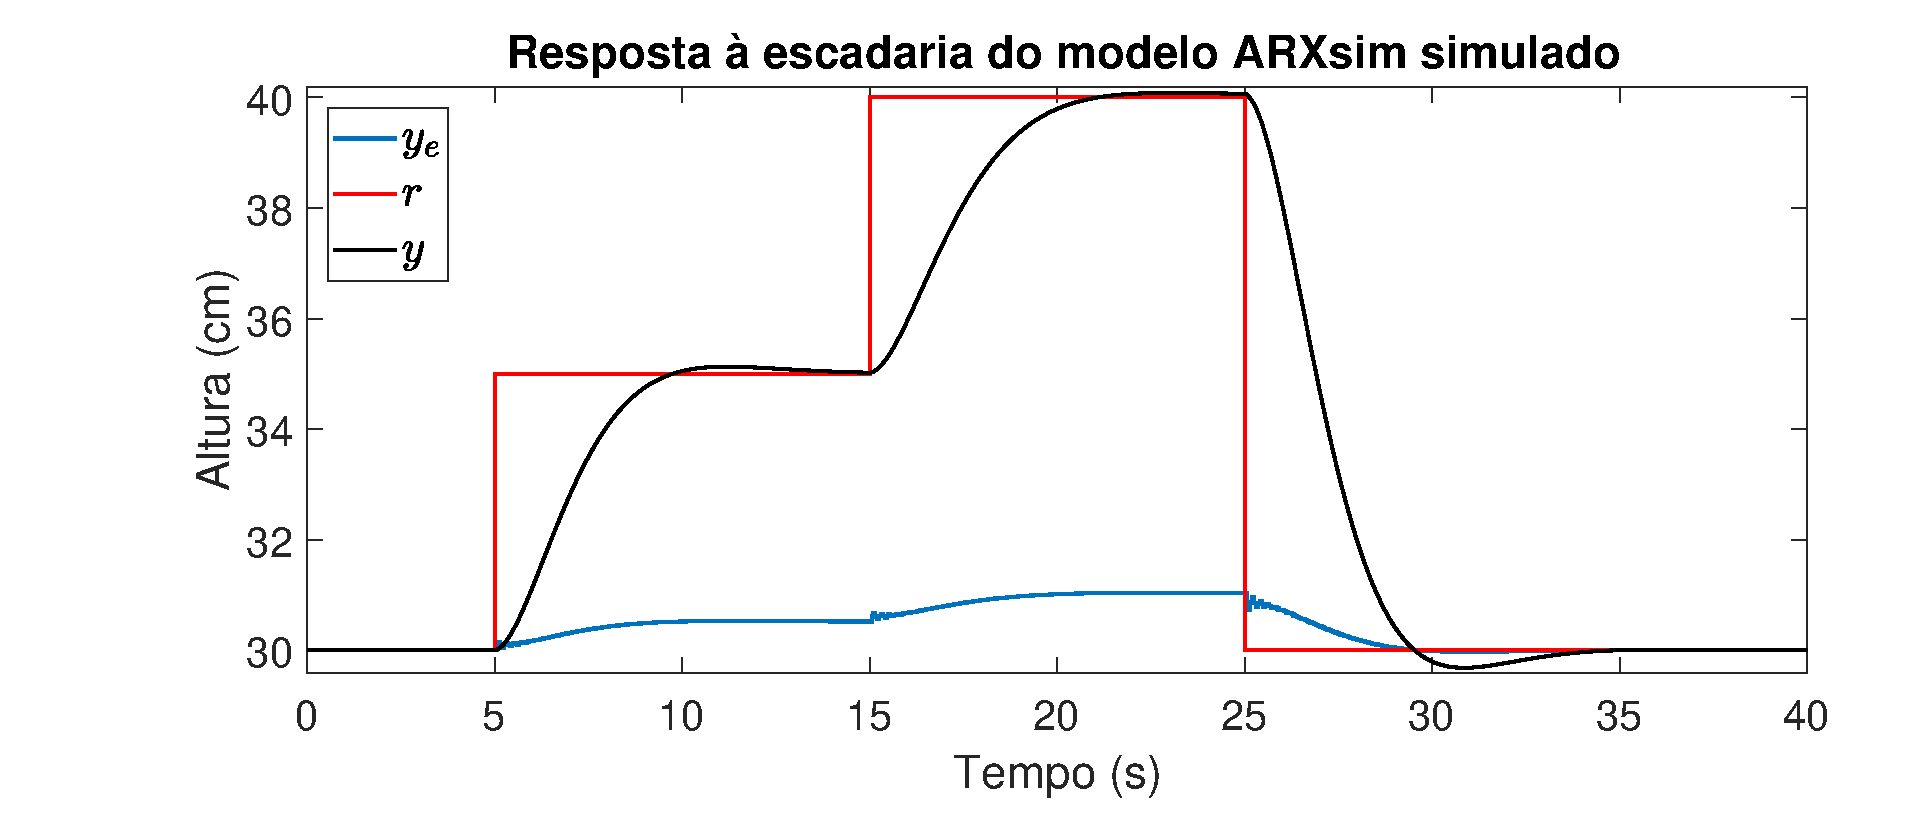
\includegraphics[width=1\linewidth]{pasta1_figuras/stairsarxsimy}
		\caption[$y_{estimado}$ e $y_{medido}$ do modelo $ARX2$]{$y_{estimado}$ e $y_{medido}$ do modelo $ARXsim$}
		\label{fig:stairsarxsimy}
	\end{subfigure}
	~ %add desired spacing between images, e. g. ~, \quad, \qquad, \hfill etc. 
	%(or a blank line to force the subfigure onto a new line)
	\begin{subfigure}[t]{0.48\textwidth}
		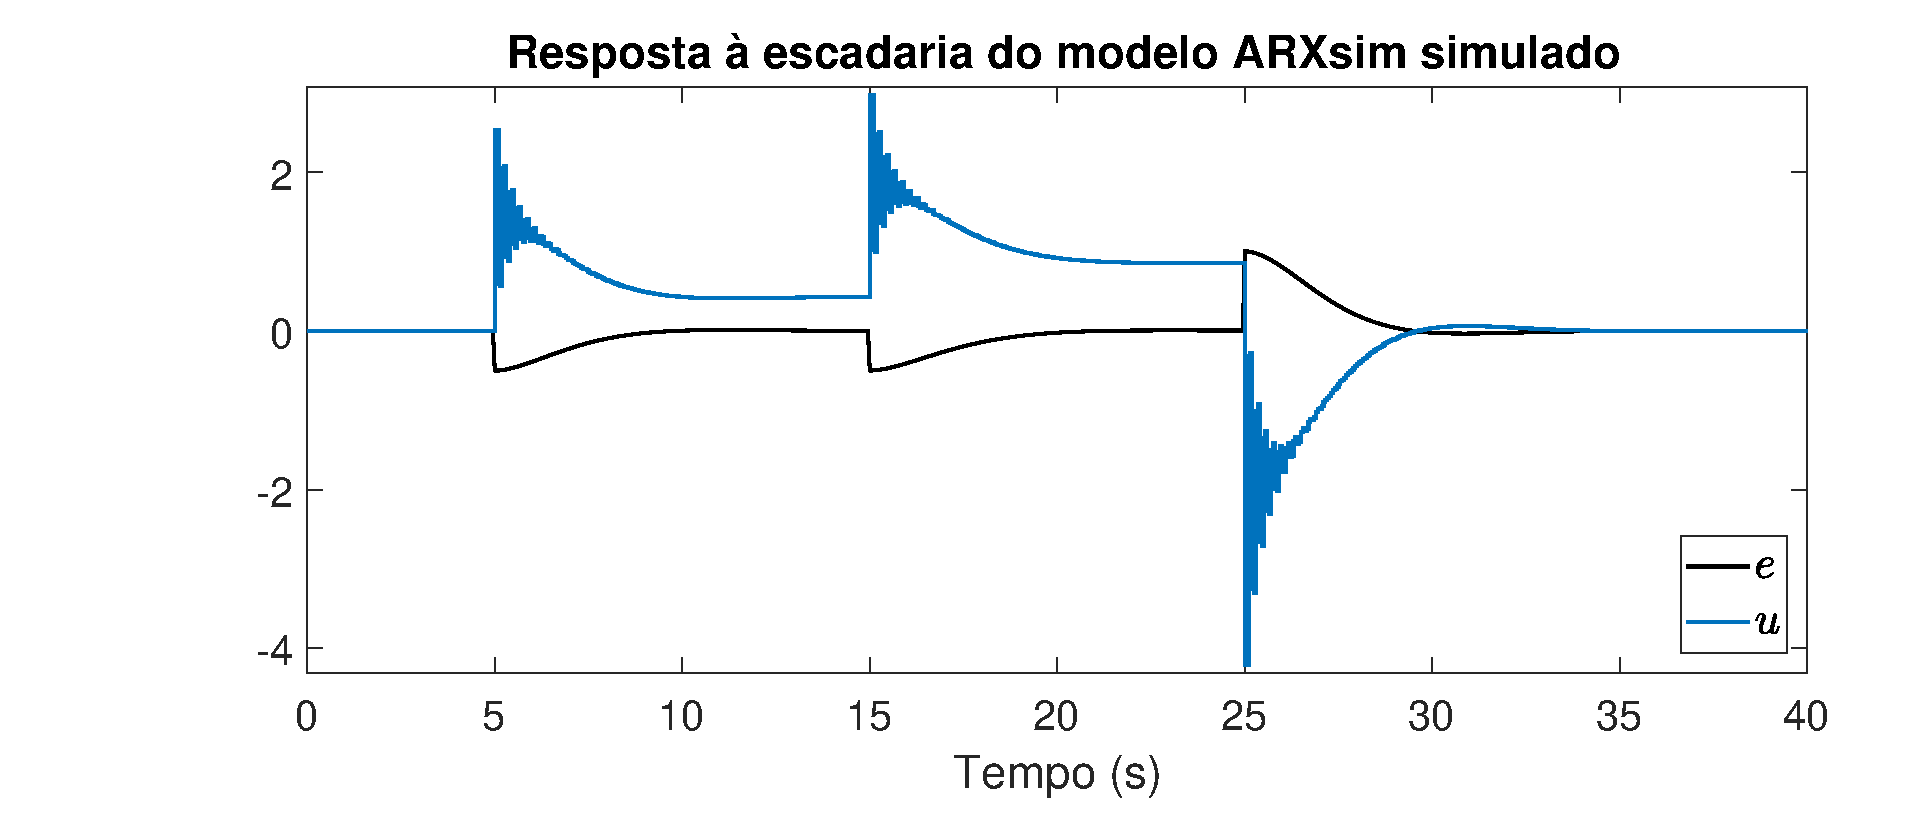
\includegraphics[width=1\linewidth]{pasta1_figuras/stairsarxsime}
		\caption[erro $e$ e sinal de controle $u$ do controlador $ARX2$]{erro $e$ e sinal de controle $u$ do controlador $ARXsim$}
		\label{fig:stairsarxsime}
	\end{subfigure}
	~ %add desired spacing between images, e. g. ~, \quad, \qquad, \hfill etc. 
	%(or a blank line to force the subfigure onto a new line)
	
	\caption{Resposta à escadaria do sistema com o controlador do modelo $ARXsim$}\label{fig:stairsarxsim}
\end{figure}

\subsubsection{Erro do Estimador} \label{erroest}
 É interessante verificar aqui o funcionamento dos estimadores projetados quando aplicados no sistema real. Na figura \ref{fig:errosub1}, vemos que o estimador do modelo $SUB1$ teve problemas para estimar a posição da bola, mas os estimadores dos modelos $ARX1$ e $ARX2$ (figuras \ref{fig:erroarx1} e \ref{fig:erroarx2}), tem um erro baixo, o que é de se esperar visto que a identificação por mínimos quadrados é um estimador ótimo, e reduz o resíduo. A tabela \ref{tb:iseestim} mostra o índice ISE do erro de estimação e nos confirma que os estimadores dos modelos ARX foram melhores que o estimador do modelo $SUB1$.
 
 \begin{table}[htb]
 	\centering
 	\begin{tabular}{|c|c|c|c|}
 		\hline 
 		& $SUB1$ & $ARX1$ & $ARX2$ \\ 
 		\hline 
 		ISE & 5.3315 & 0.5193 & 0.6134 \\ 
 		\hline 
 	\end{tabular} 
 \caption{Tabela com índices ISE do erro de estimação}
 \label{tb:iseestim}
 \end{table}
 
 
\begin{figure}[htb]
	\centering
	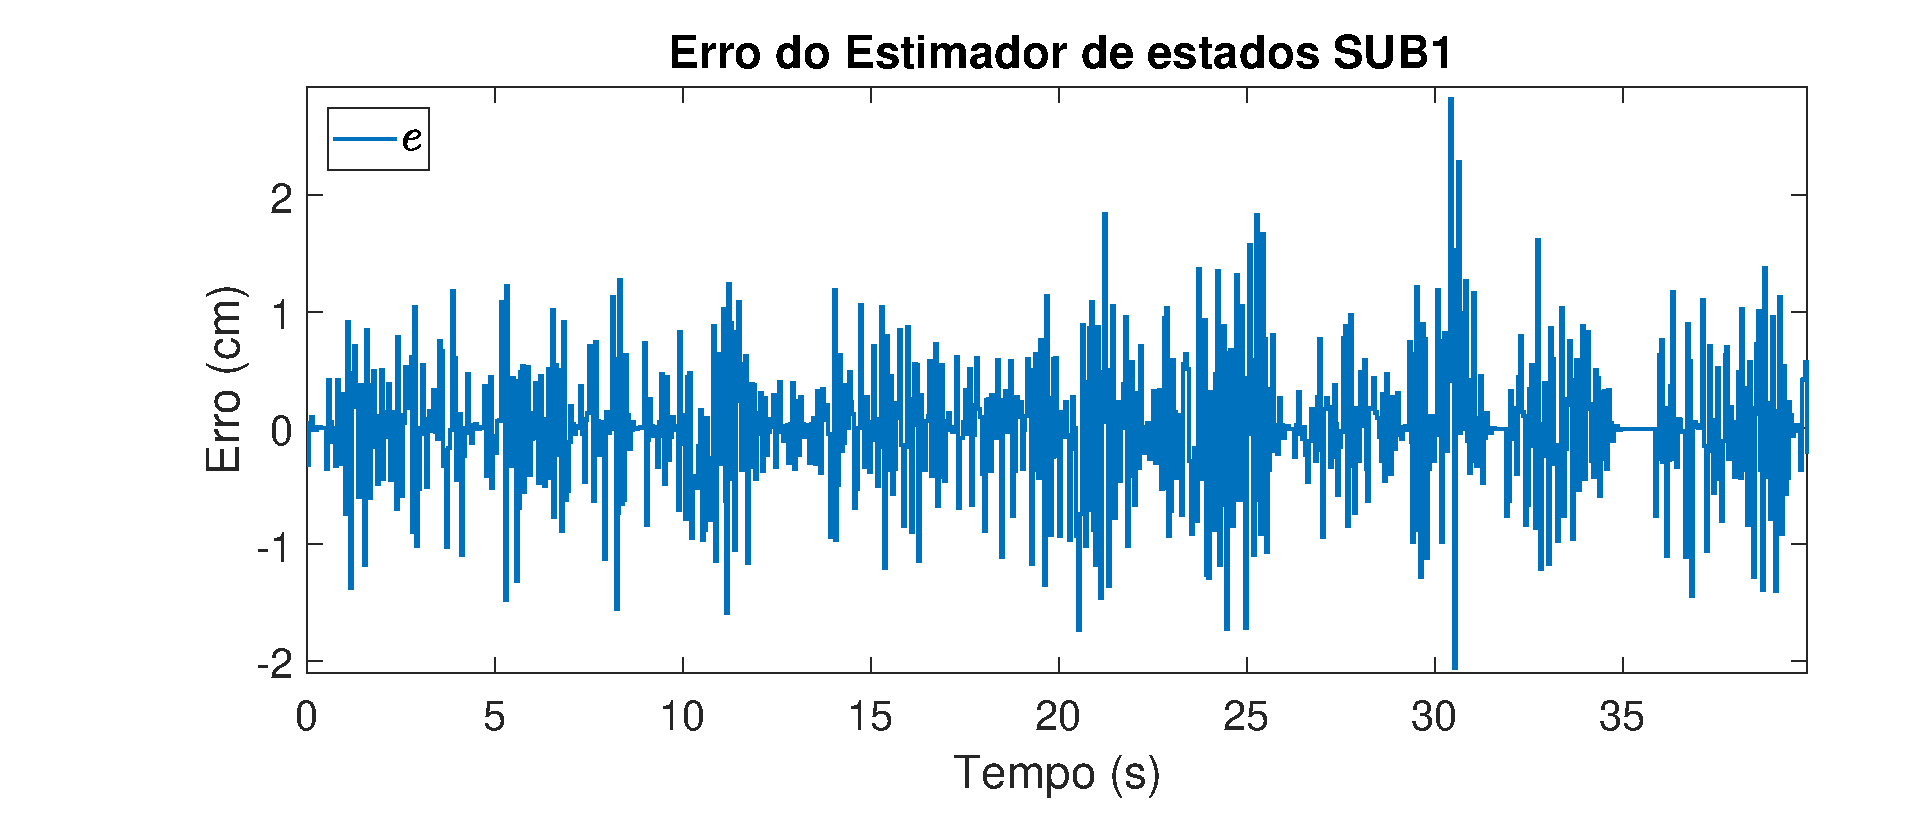
\includegraphics[width=1\linewidth]{errosub1}
	\caption[Erro do estimador do modelo $SUB1$ na resposta à escadaria]{Erro do estimador do modelo $SUB1$ na resposta à escadaria}
	\label{fig:errosub1}
\end{figure}

\begin{figure}[htb]
	\centering
	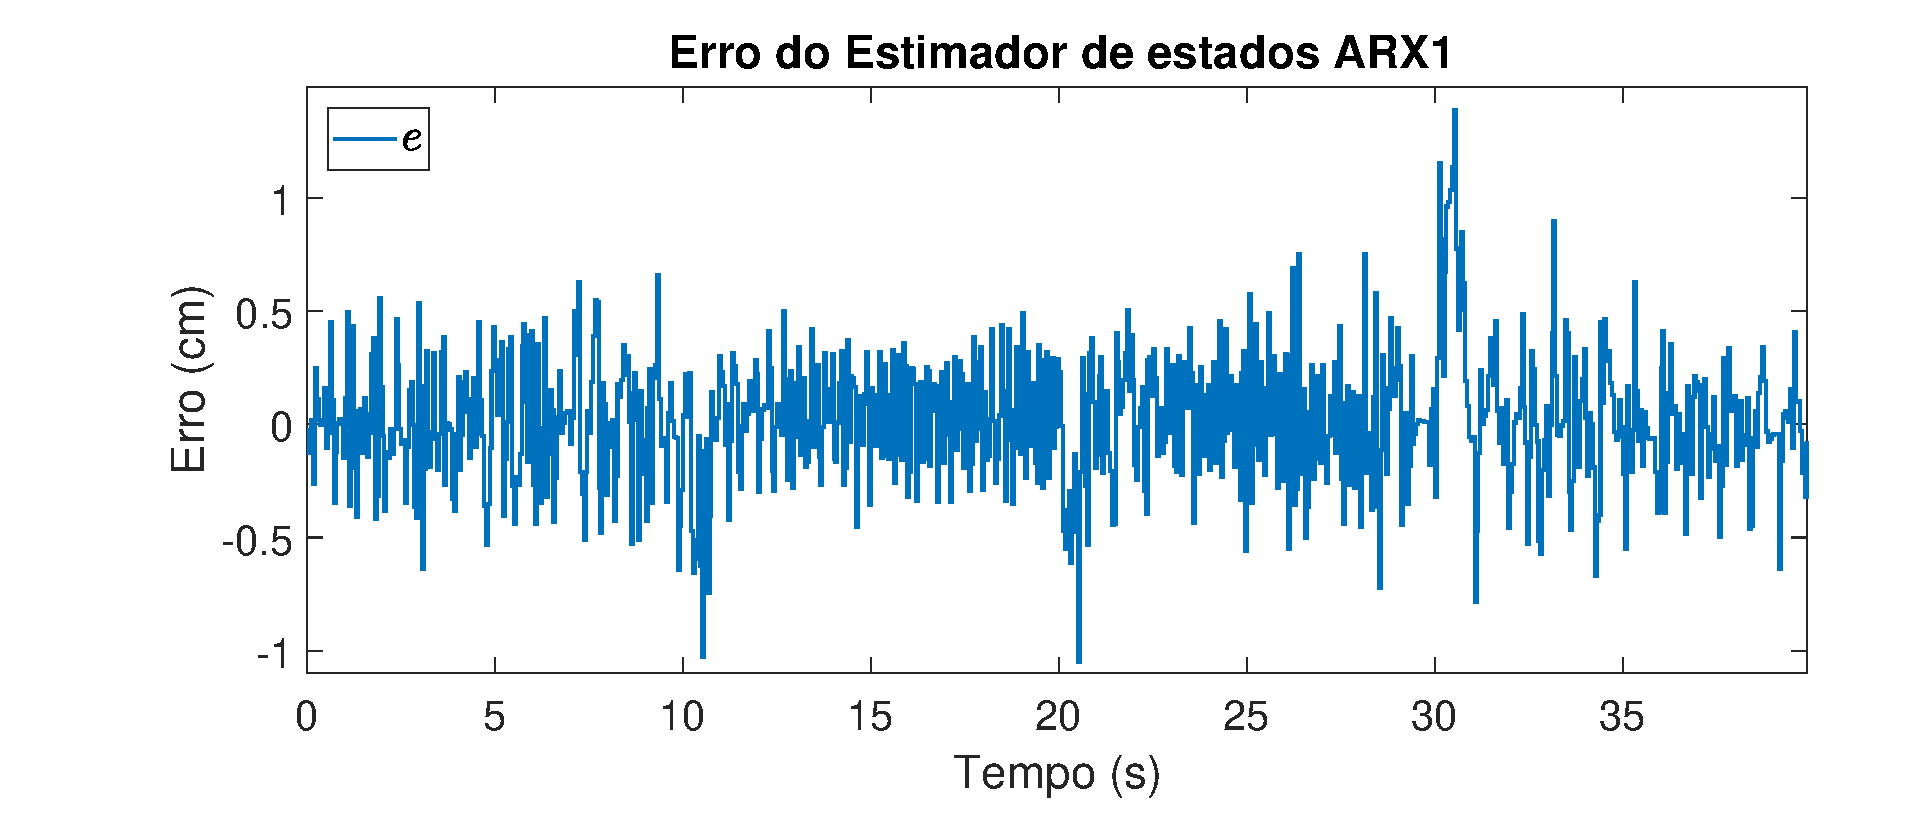
\includegraphics[width=1\linewidth]{erroarx1}
	\caption[Erro do estimador do modelo $ARX1$ na resposta à escadaria]{Erro do estimador do modelo $ARX1$ na resposta à escadaria}
	\label{fig:erroarx1}
\end{figure}

\begin{figure}[htb]
	\centering
	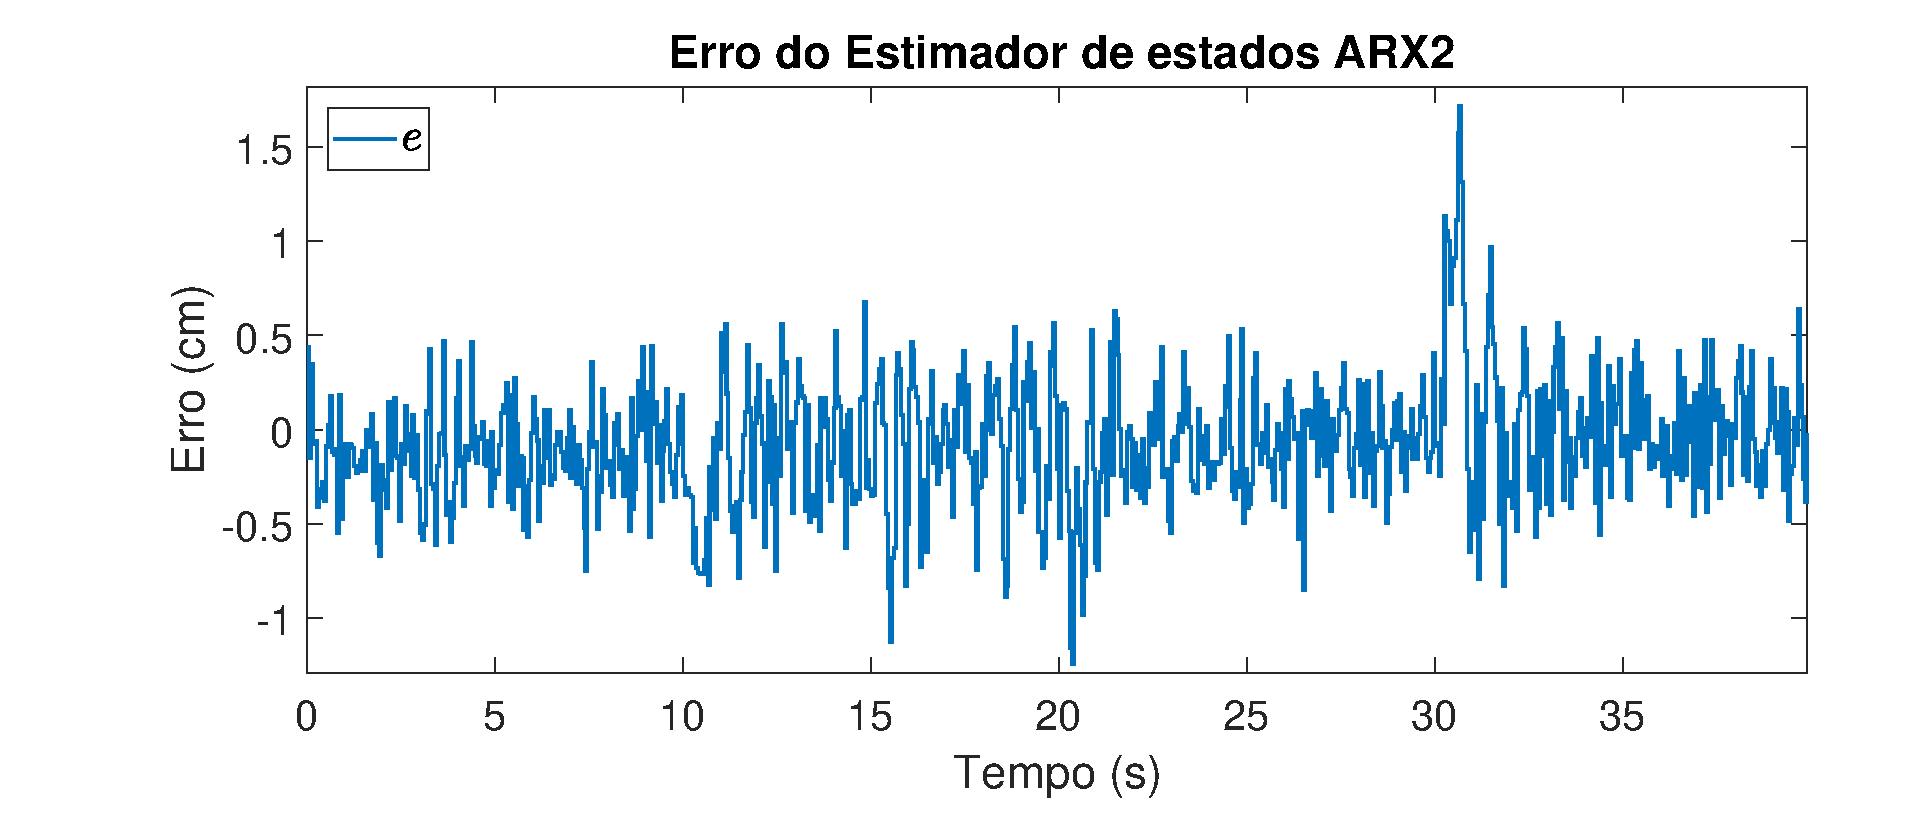
\includegraphics[width=1\linewidth]{erroarx2}
	\caption[Erro do estimador do modelo $ARX2$ na resposta à escadaria]{Erro do estimador do modelo $ARX2$ na resposta à escadaria}
	\label{fig:erroarx2}
\end{figure}

Vemos que os estimadores dos dois modelos ARX, ao serem aplicados no sistema, tiveram um bom desempenho (figuras \ref{fig:erroarx1} e \ref{fig:erroarx2}), permanecendo abaixo de 1 cm de diferença com algumas exceções, que atribuímos ao ruído do sensor. O estimador do modelo $SUB1$ não apresentou bom desempenho, mostrando erros superiores a 1 cm com frequência.


\subsection{Resultados do Teste de Robustez à mudança de Parâmetros}\label{rmp}

\subsubsection{Modelo $SUB1$}
Testamos a robustez do modelo $SUB1$ à mudança de parâmetros com o sistema real e vemos na figura \ref{fig:mprsub1y} que ele não conseguiu seguir a referência quando aumentamos o peso da bola.
\begin{figure}[htb]
	\centering
	\begin{subfigure}[t]{0.48\textwidth}
		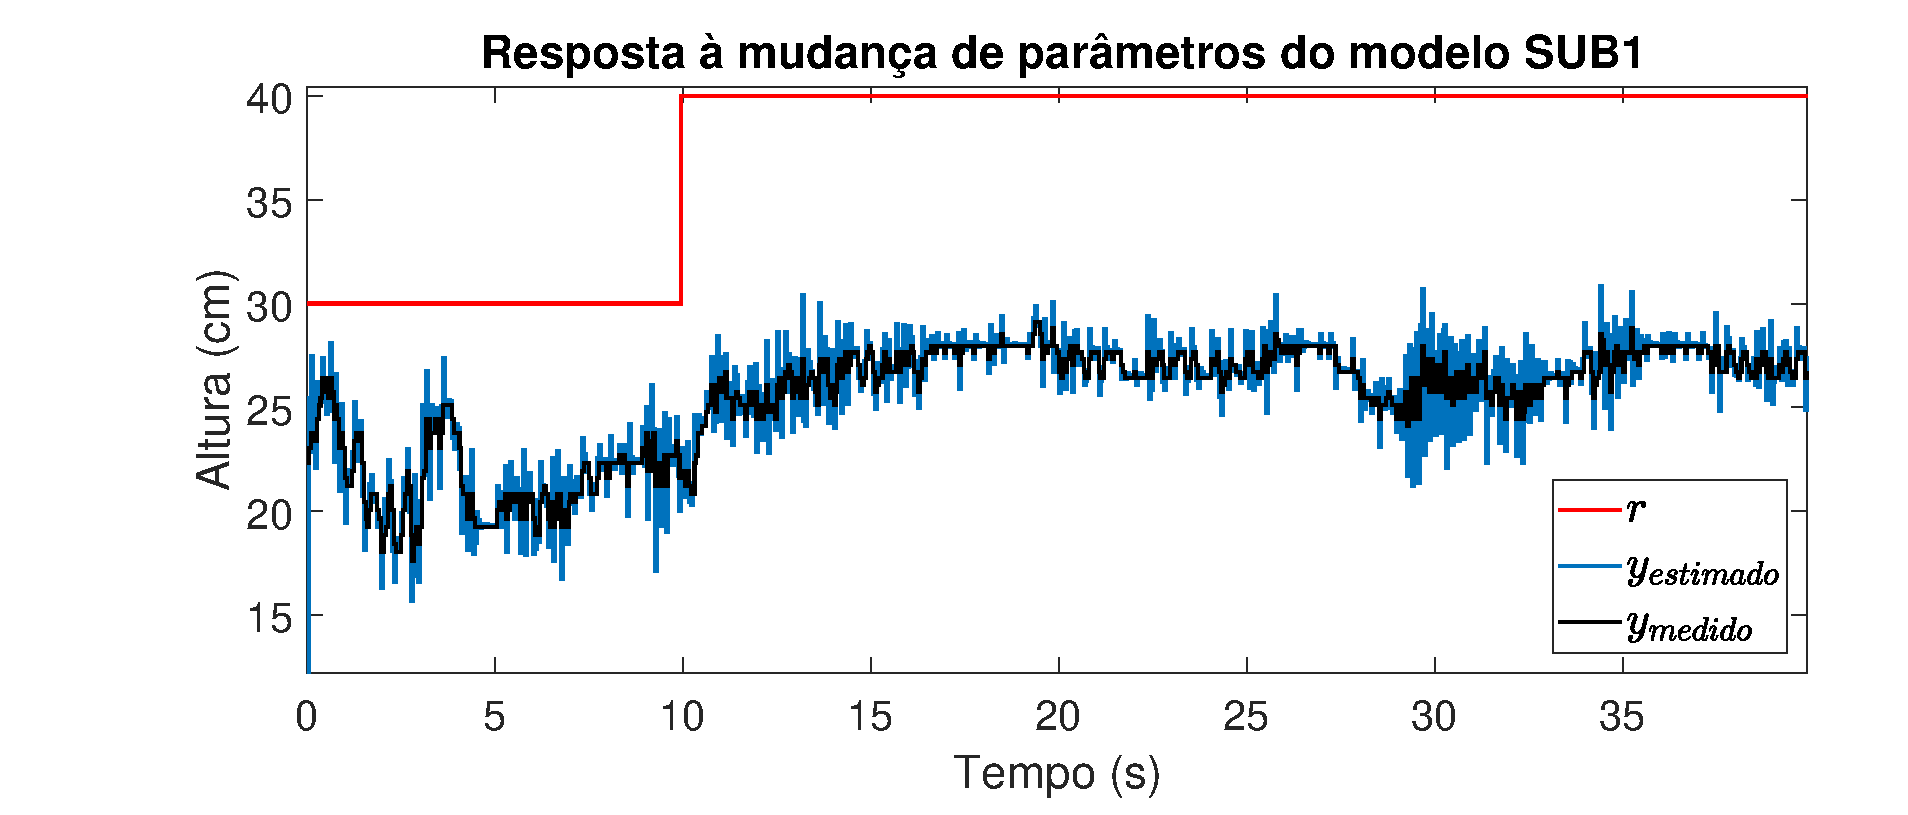
\includegraphics[width=1\linewidth]{mprsub1y}
		\caption[$y_{estimado}$ e $y_{medido}$ do modelo $SUB1$]{$y_{estimado}$ e $y_{medido}$ do modelo $SUB1$}
		\label{fig:mprsub1y}
	\end{subfigure}
	~ %add desired spacing between images, e. g. ~, \quad, \qquad, \hfill etc. 
	%(or a blank line to force the subfigure onto a new line)
	\begin{subfigure}[t]{0.48\textwidth}
		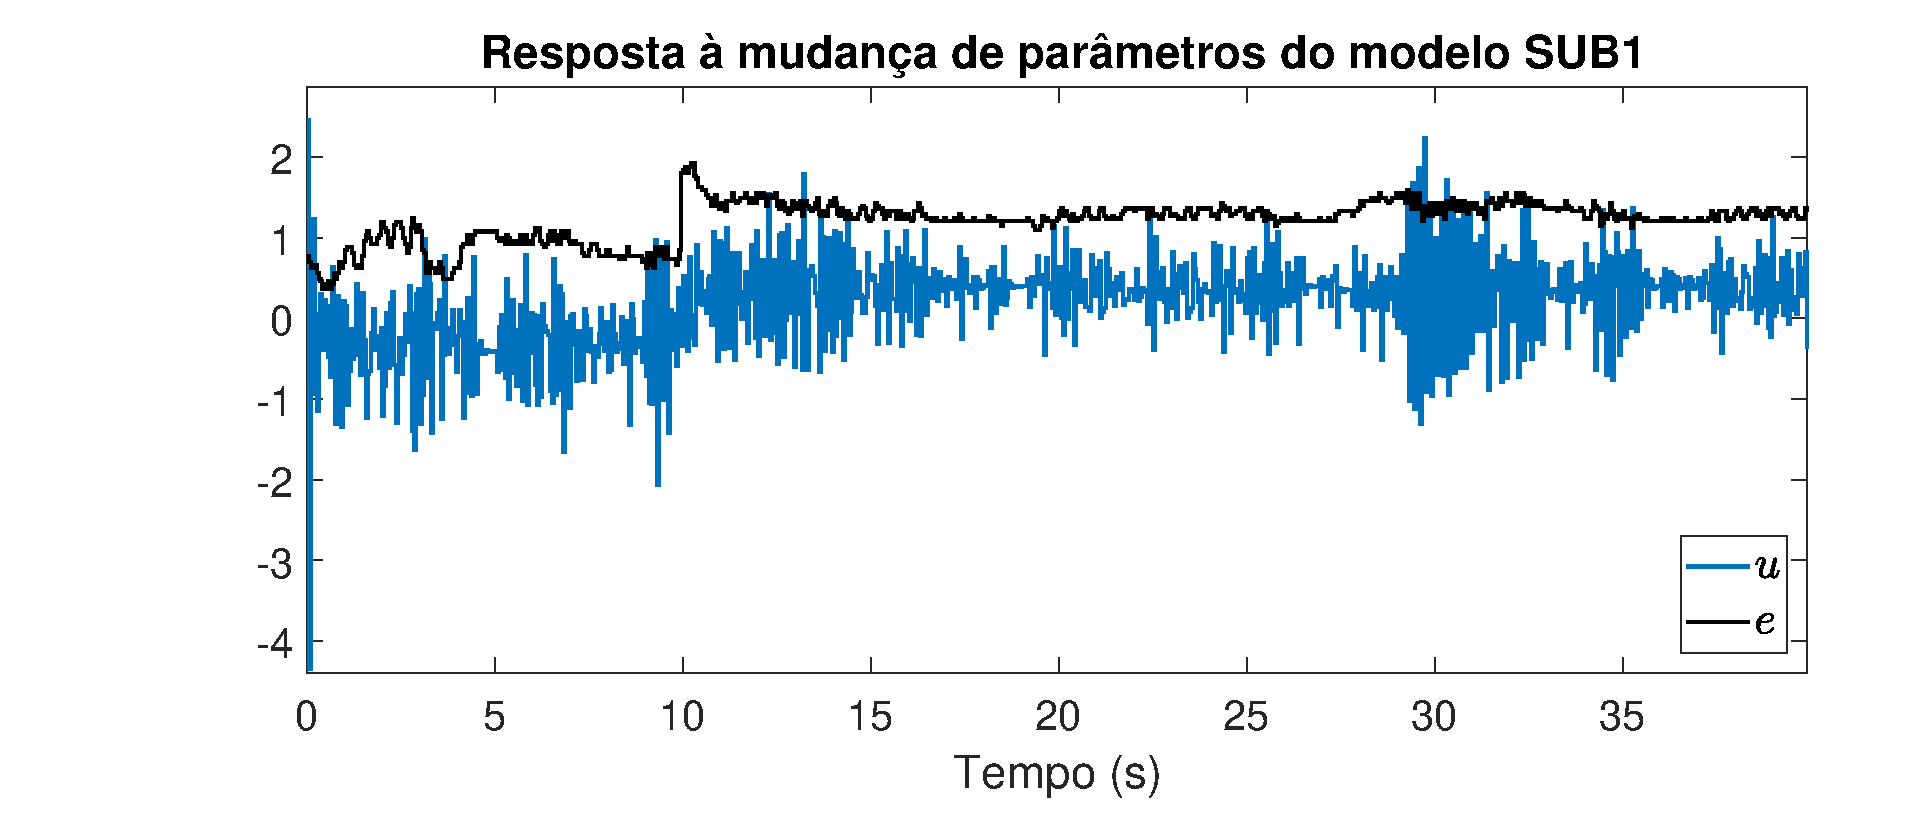
\includegraphics[width=1\linewidth]{mprsub1e}
		\caption[erro $e$ e sinal de controle $u$ do controlador $SUB1$]{erro $e$ e sinal de controle $u$ do controlador $SUB1$}
		\label{fig:mprsub1e}
	\end{subfigure}
	~ %add desired spacing between images, e. g. ~, \quad, \qquad, \hfill etc. 
	%(or a blank line to force the subfigure onto a new line)
	
	\caption{Resposta do sistema com o controlador do modelo $SUB1$ com mudança de parâmetros}\label{fig:mprsub1}
\end{figure}

\subsubsection{Modelo $ARX1$}
Testamos a robustez do modelo $ARX1$ à mudança de parâmetros com o sistema real e, como no modelo $SUB1$, ele não conseguiu seguir a referência (figura \ref{fig:mprarx1y}).
\begin{figure}[htb]
	\centering
	\begin{subfigure}[t]{0.48\textwidth}
		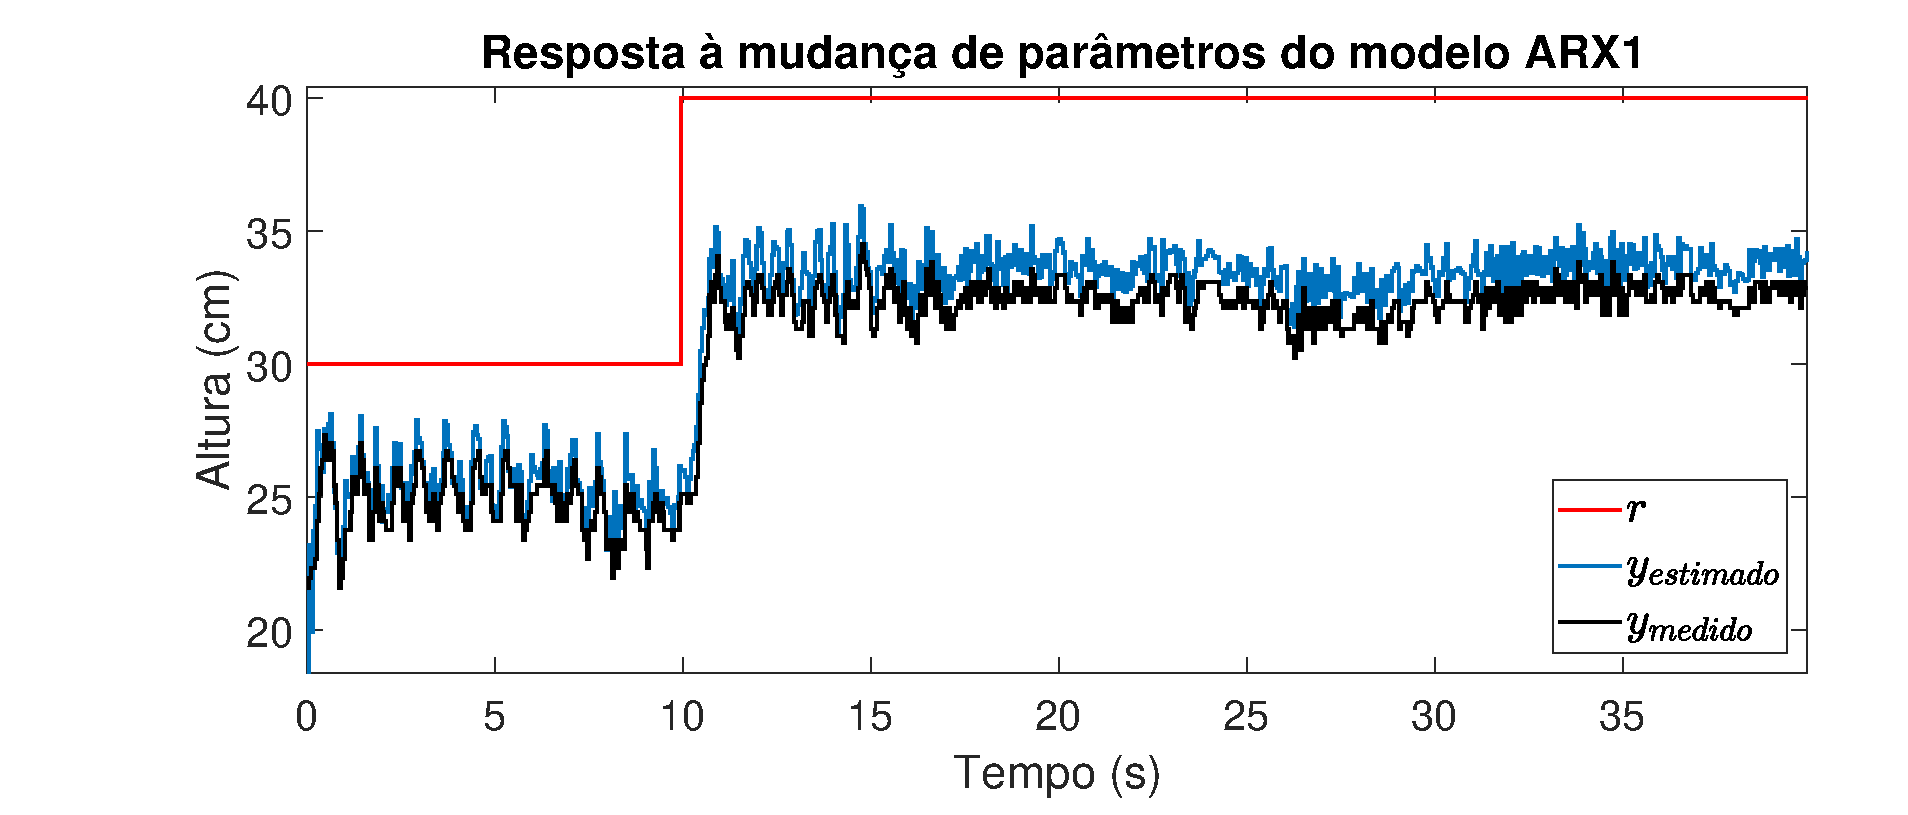
\includegraphics[width=1\linewidth]{mprarx1y}
		\caption[$y_{estimado}$ e $y_{medido}$ do modelo $ARX1$]{$y_{estimado}$ e $y_{medido}$ do modelo $ARX1$}
		\label{fig:mprarx1y}
	\end{subfigure}
	~ %add desired spacing between images, e. g. ~, \quad, \qquad, \hfill etc. 
	%(or a blank line to force the subfigure onto a new line)
	\begin{subfigure}[t]{0.48\textwidth}
		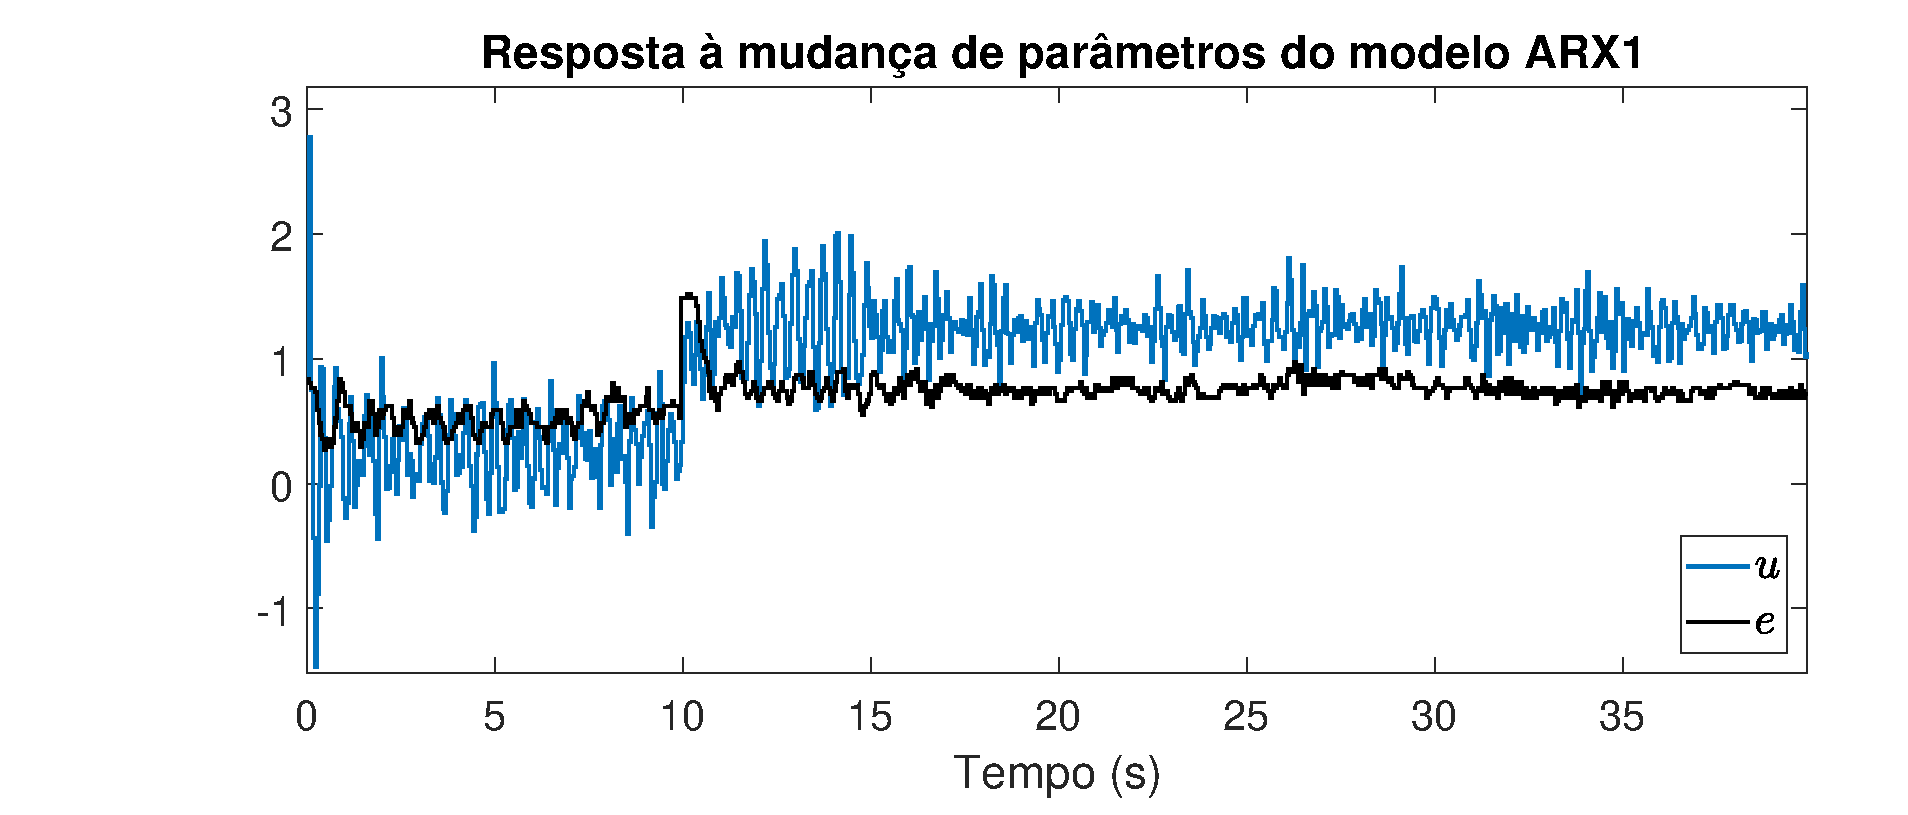
\includegraphics[width=1\linewidth]{mprarx1e}
		\caption[erro $e$ e sinal de controle $u$ do controlador $ARX1$]{erro $e$ e sinal de controle $u$ do controlador $ARX1$}
		\label{fig:mprarx1e}
	\end{subfigure}
	~ %add desired spacing between images, e. g. ~, \quad, \qquad, \hfill etc. 
	%(or a blank line to force the subfigure onto a new line)
	
	\caption{Resposta do sistema com o controlador do modelo $ARX1$ com mudança de parâmetros}\label{fig:mprarx1}
\end{figure}

\subsubsection{Modelo $ARX2$}
O modelo $ARX2$ também não conseguiu seguir a referência (figura \ref{fig:mprarx2y}).
\begin{figure}[htb]
	\centering
	\begin{subfigure}[t]{0.48\textwidth}
		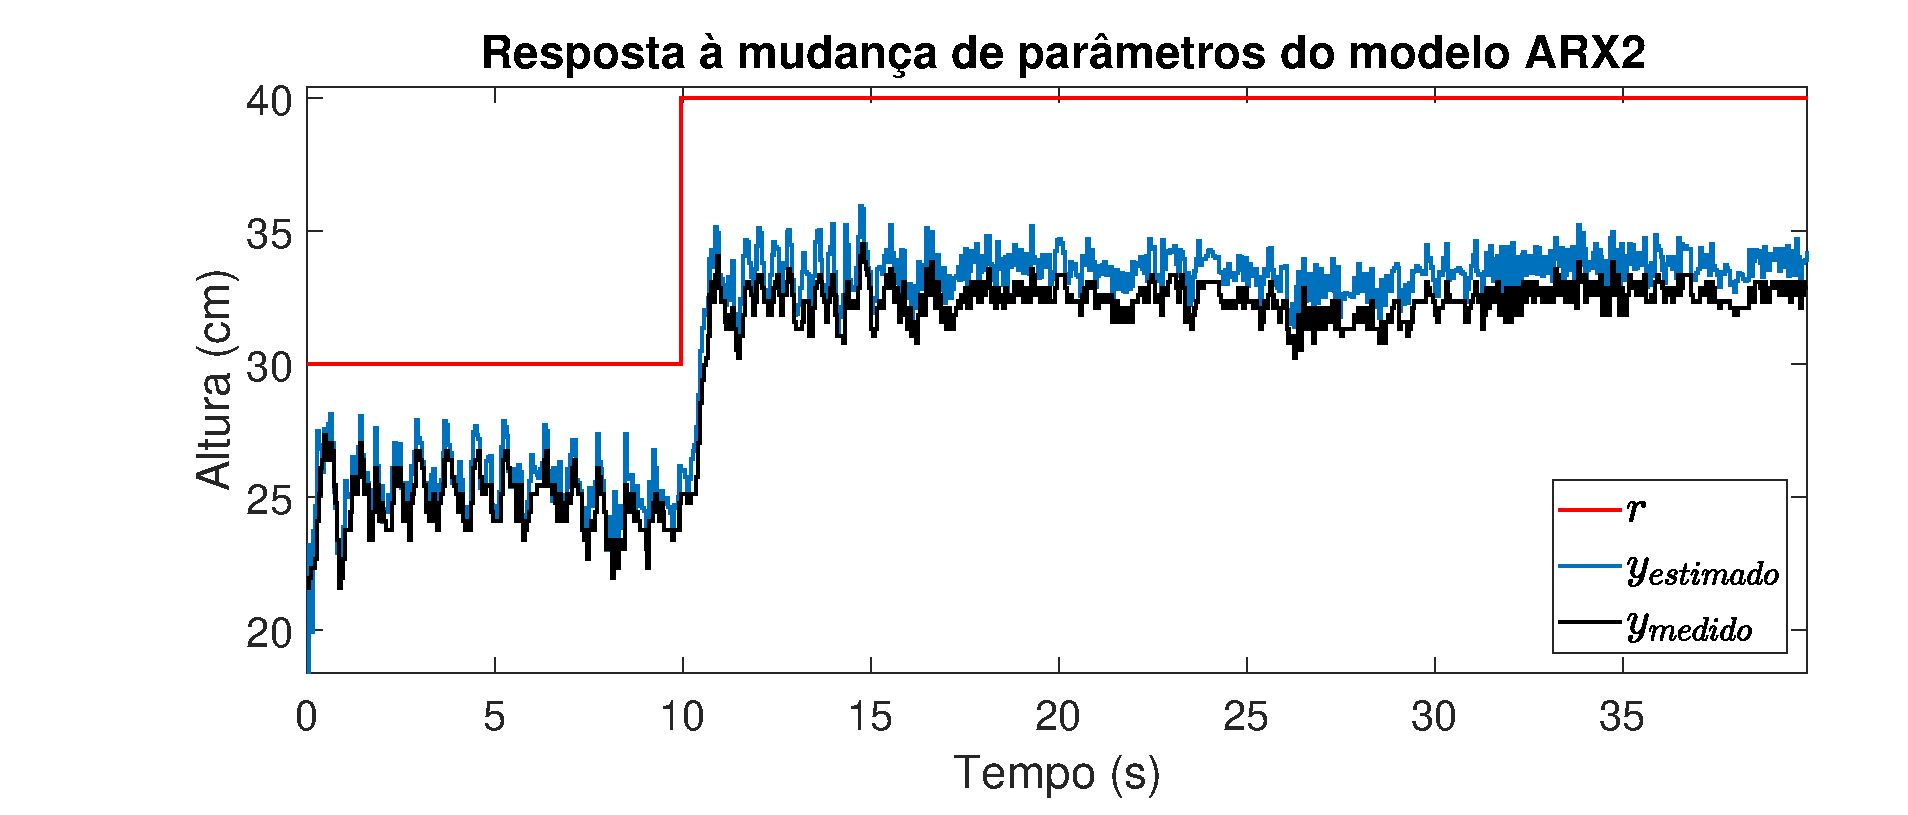
\includegraphics[width=1\linewidth]{mprarx2y}
		\caption[$y_{estimado}$ e $y_{medido}$ do modelo $ARX2$]{$y_{estimado}$ e $y_{medido}$ do modelo $ARX2$}
		\label{fig:mprarx2y}
	\end{subfigure}
	~ %add desired spacing between images, e. g. ~, \quad, \qquad, \hfill etc. 
	%(or a blank line to force the subfigure onto a new line)
	\begin{subfigure}[t]{0.48\textwidth}
		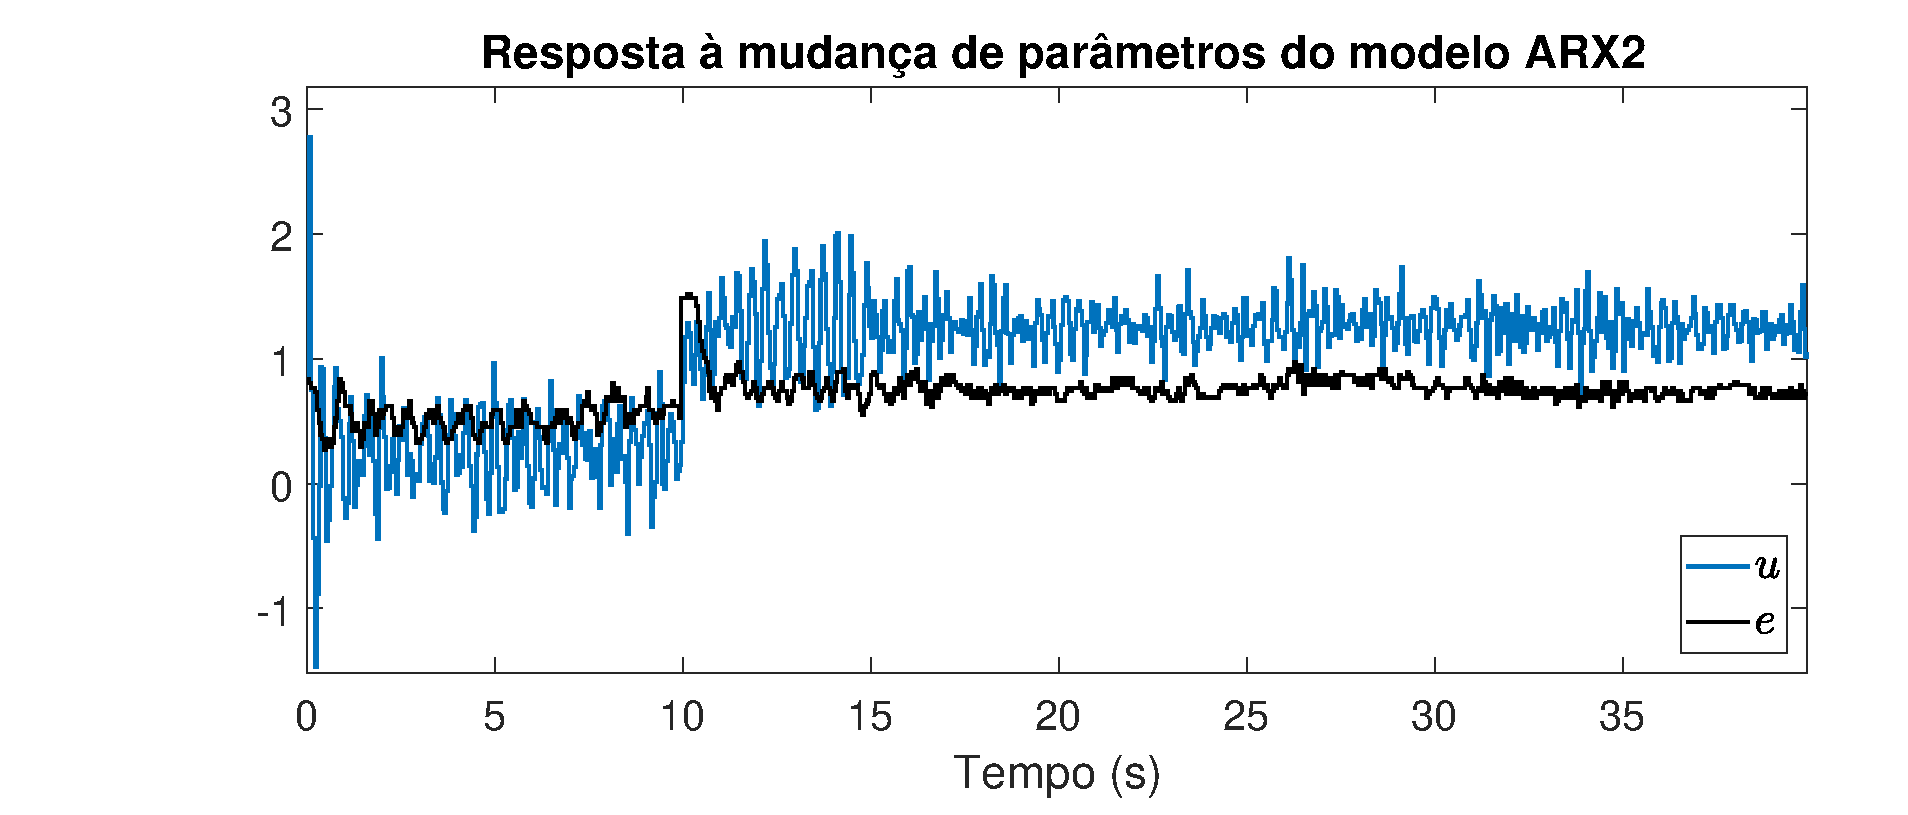
\includegraphics[width=1\linewidth]{mprarx2e}
		\caption[erro $e$ e sinal de controle $u$ do controlador $ARX2$]{erro $e$ e sinal de controle $u$ do controlador $ARX2$}
		\label{fig:mprarx2e}
	\end{subfigure}
	~ %add desired spacing between images, e. g. ~, \quad, \qquad, \hfill etc. 
	%(or a blank line to force the subfigure onto a new line)
	
	\caption{Resposta do sistema com o controlador do modelo $ARX2$ com mudança de parâmetros}\label{fig:mprarx2}
\end{figure}

\subsubsection{Modelo $ARXsim$}

Mudamos o peso da bola para o modelo $ARXsim$ e testamos a sua resposta ao degrau. Vemos na figura \ref{fig:mpsarxsimy}, que o sistema simulado não foi capaz de responder à mudança de parâmetros.

\begin{figure}[htb]
	\centering
	\begin{subfigure}[t]{0.48\textwidth}
		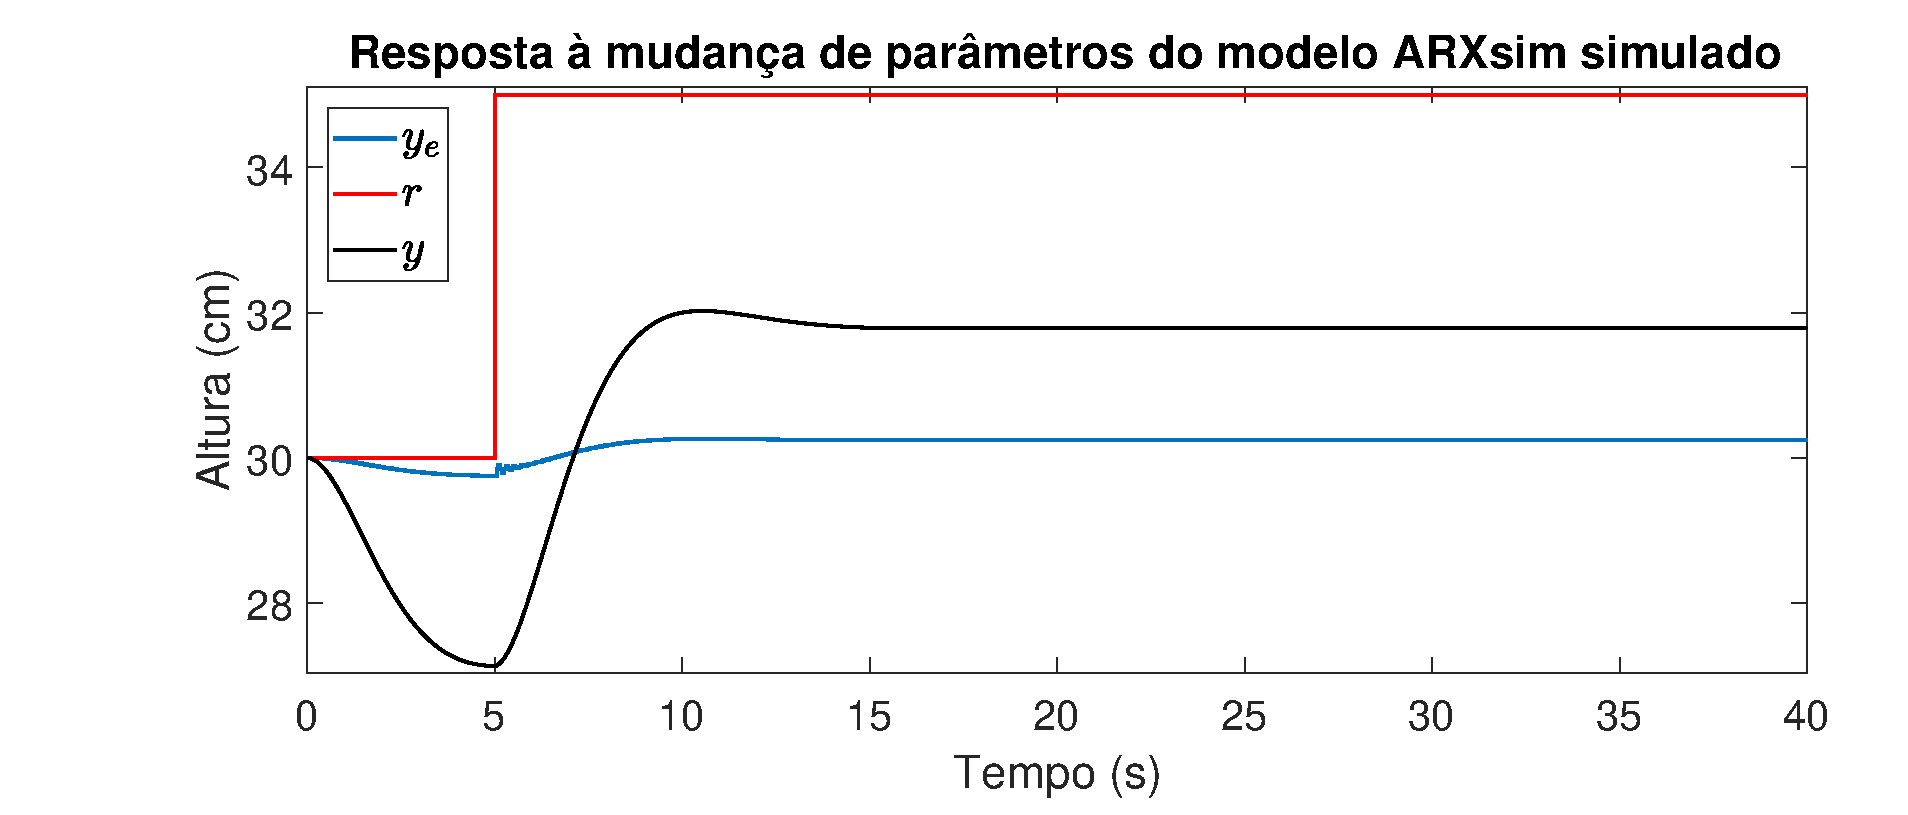
\includegraphics[width=1\linewidth]{pasta1_figuras/mpsarxsimy}
		\caption[$y_{estimado}$ e $y_{medido}$ do modelo $ARX2$]{$y_{estimado}$ e $y_{medido}$ do modelo $ARXsim$}
		\label{fig:mpsarxsimy}
	\end{subfigure}
	~ %add desired spacing between images, e. g. ~, \quad, \qquad, \hfill etc. 
	%(or a blank line to force the subfigure onto a new line)
	\begin{subfigure}[t]{0.48\textwidth}
		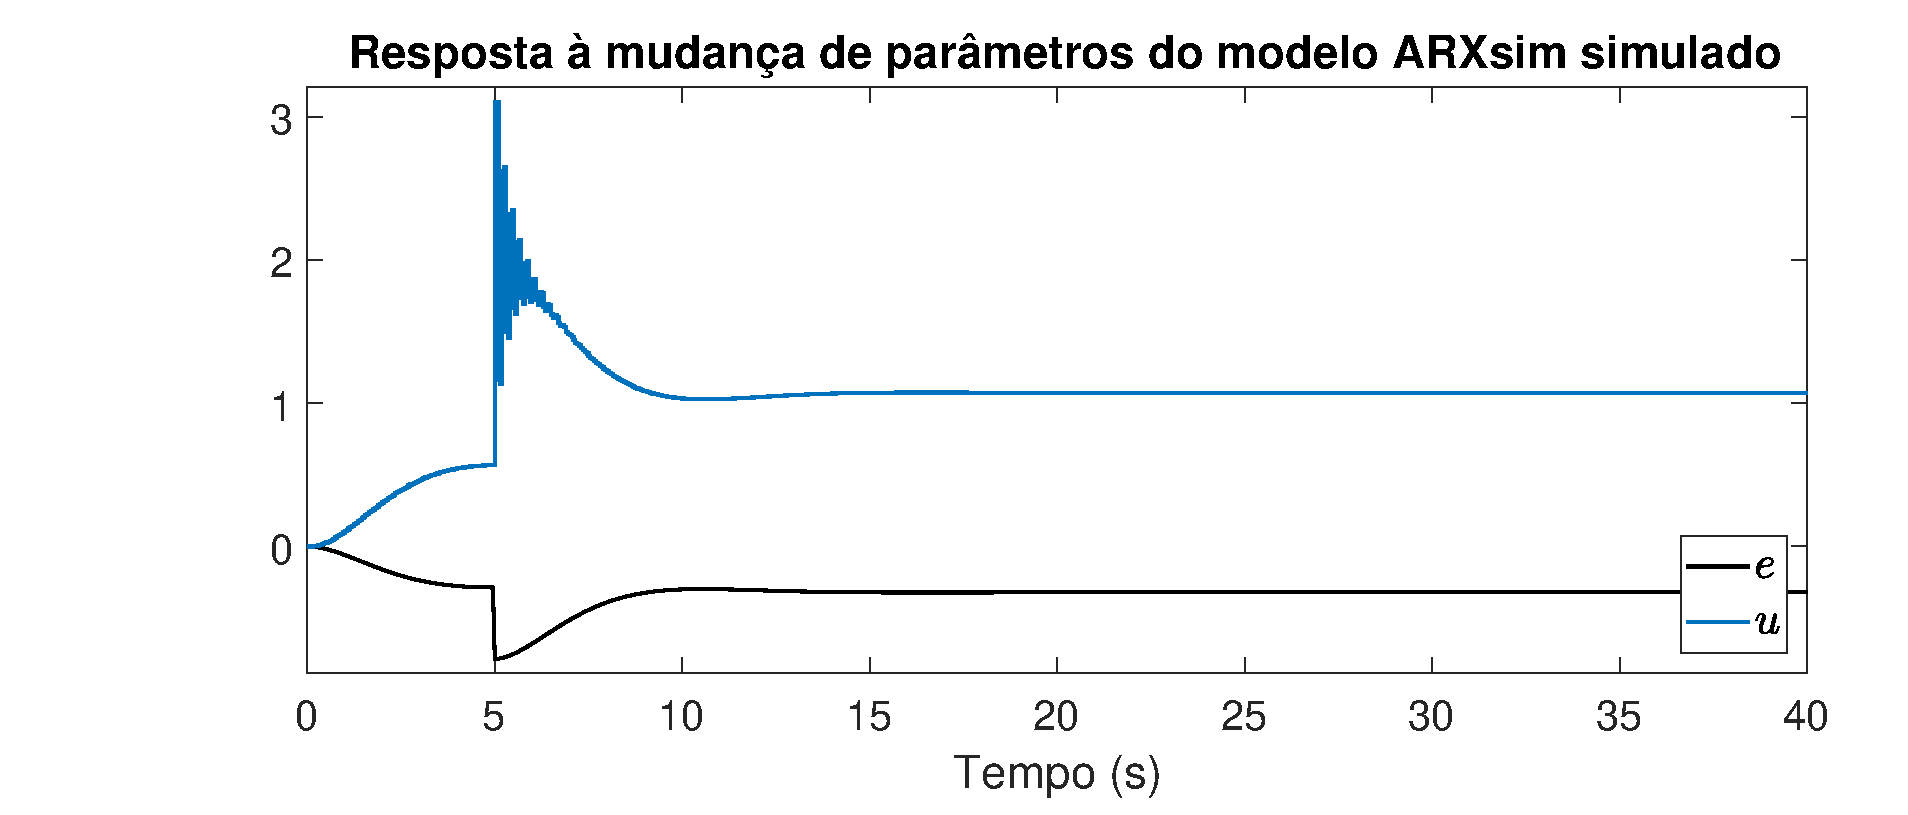
\includegraphics[width=1\linewidth]{pasta1_figuras/mpsarxsime}
		\caption[erro $e$ e sinal de controle $u$ do controlador $ARX2$]{erro $e$ e sinal de controle $u$ do controlador $ARXsim$}
		\label{fig:mpsarxsime}
	\end{subfigure}
	~ %add desired spacing between images, e. g. ~, \quad, \qquad, \hfill etc. 
	%(or a blank line to force the subfigure onto a new line)
	
	\caption{Resposta do sistema com o controlador do modelo $ARXsim$ com mudança de parâmetros}\label{fig:mpsarxsim}
\end{figure}

\subsection{Resultados do Teste de Robustez à perturbação externa}\label{rpe}

\subsubsection{Modelo $SUB1$}
Testamos a robustez do modelo $SUB1$ à perturbação externa com o sistema real e vemos que o sistema também não conseguiu rejeitar perturbação externa (figura \ref{fig:pextrsub1y}).

\begin{figure}[htb]
	\centering
	\begin{subfigure}[t]{0.48\textwidth}
		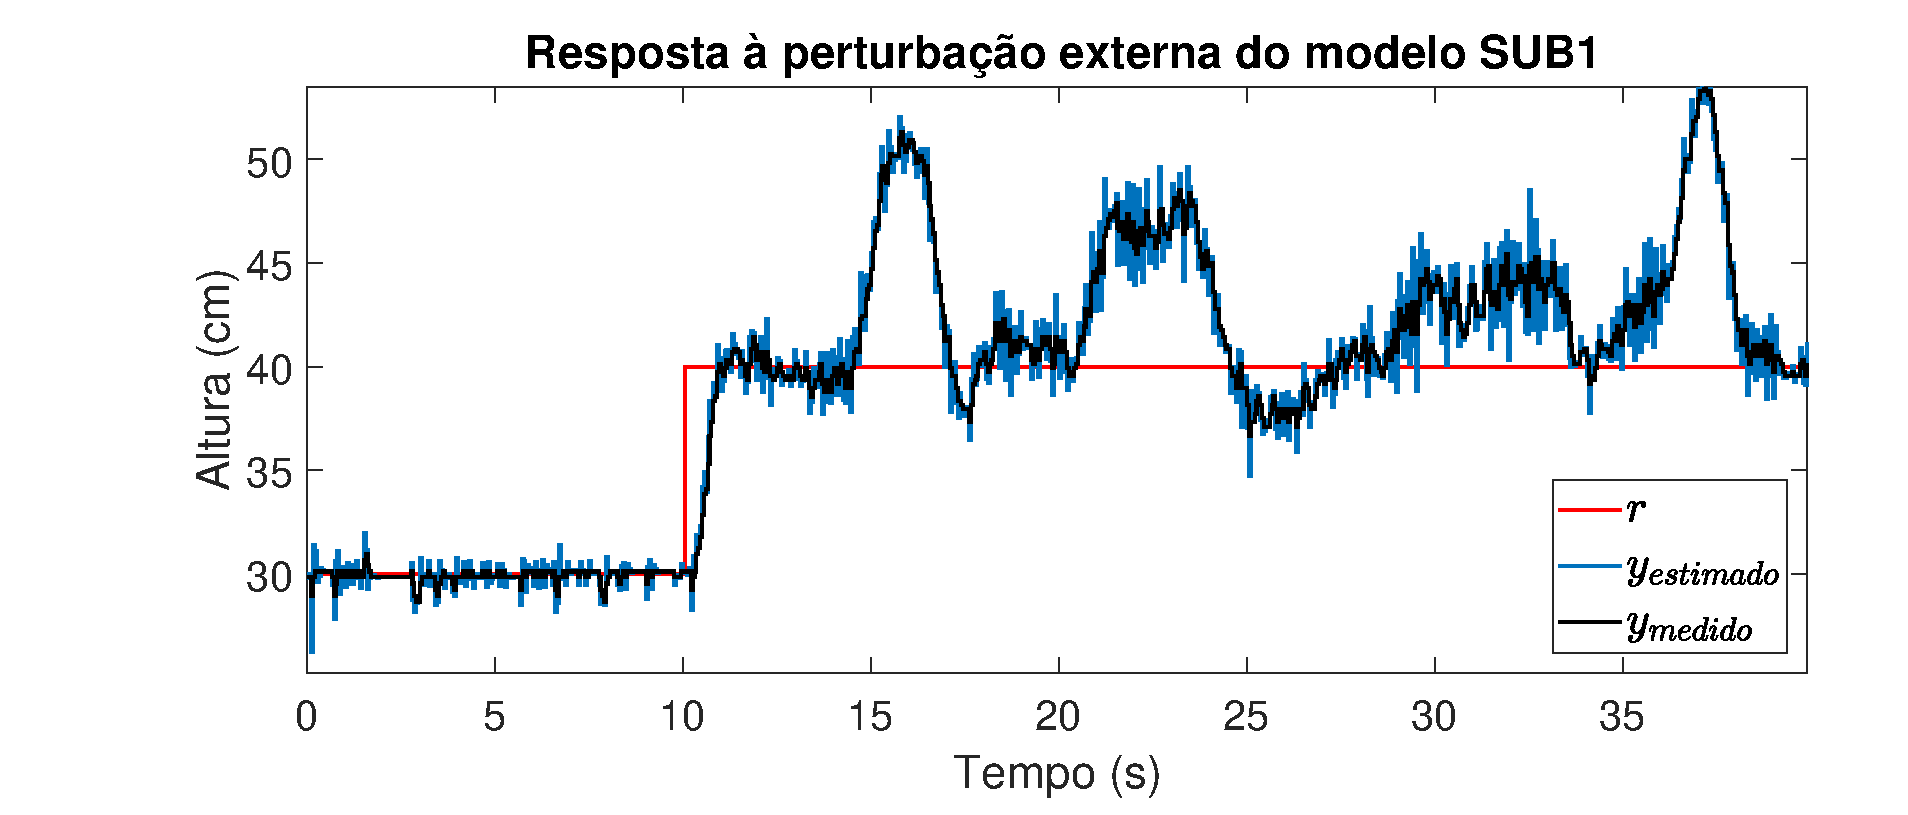
\includegraphics[width=1\linewidth]{pextrsub1y}
		\caption[$y_{estimado}$ e $y_{medido}$ do modelo $SUB1$]{$y_{estimado}$ e $y_{medido}$ do modelo $SUB1$}
		\label{fig:pextrsub1y}
	\end{subfigure}
	~ %add desired spacing between images, e. g. ~, \quad, \qquad, \hfill etc. 
	%(or a blank line to force the subfigure onto a new line)
	\begin{subfigure}[t]{0.48\textwidth}
		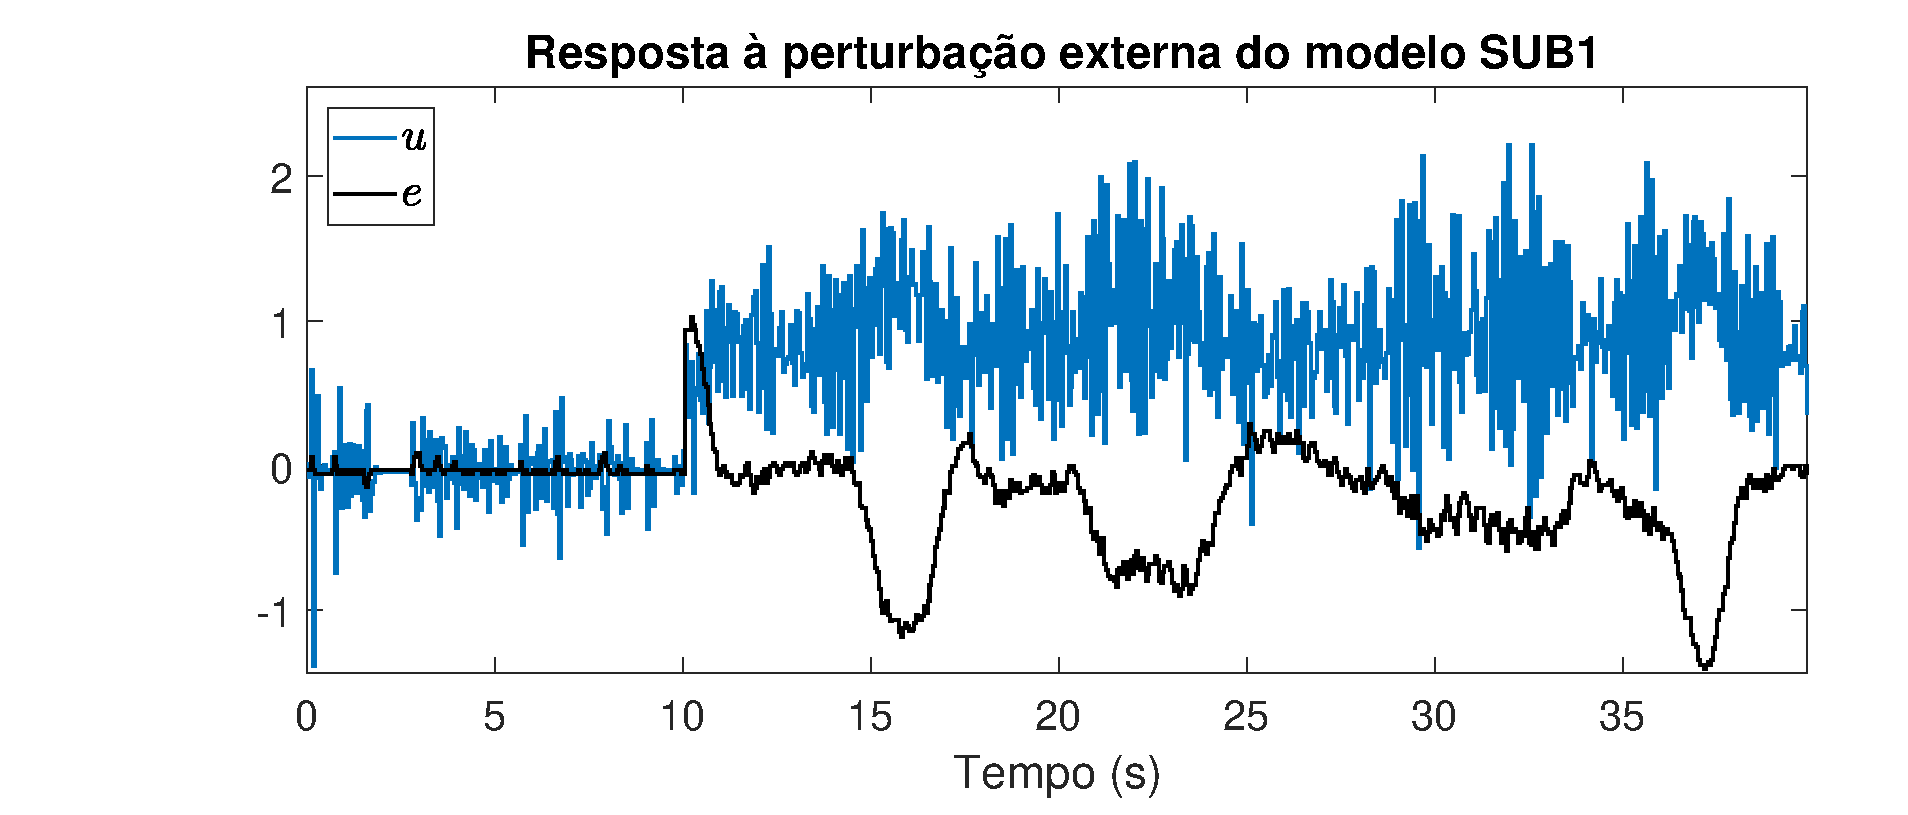
\includegraphics[width=1\linewidth]{pextrsub1e}
		\caption[erro $e$ e sinal de controle $u$ do controlador $SUB1$]{erro $e$ e sinal de controle $u$ do controlador $SUB1$}
		\label{fig:pextrsub1e}
	\end{subfigure}
	~ %add desired spacing between images, e. g. ~, \quad, \qquad, \hfill etc. 
	%(or a blank line to force the subfigure onto a new line)
	
	\caption{Resposta à perturbação externa do sistema com o controlador do modelo $SUB1$}\label{fig:pextrsub1}
\end{figure}

\subsubsection{Modelo $ARX1$}
O modelo $ARX1$ também não conseguiu seguir a referência com o aumento do peso da bola (figura \ref{fig:pextrarx1y}).
\begin{figure}[htb]
	\centering
	\begin{subfigure}[t]{0.48\textwidth}
		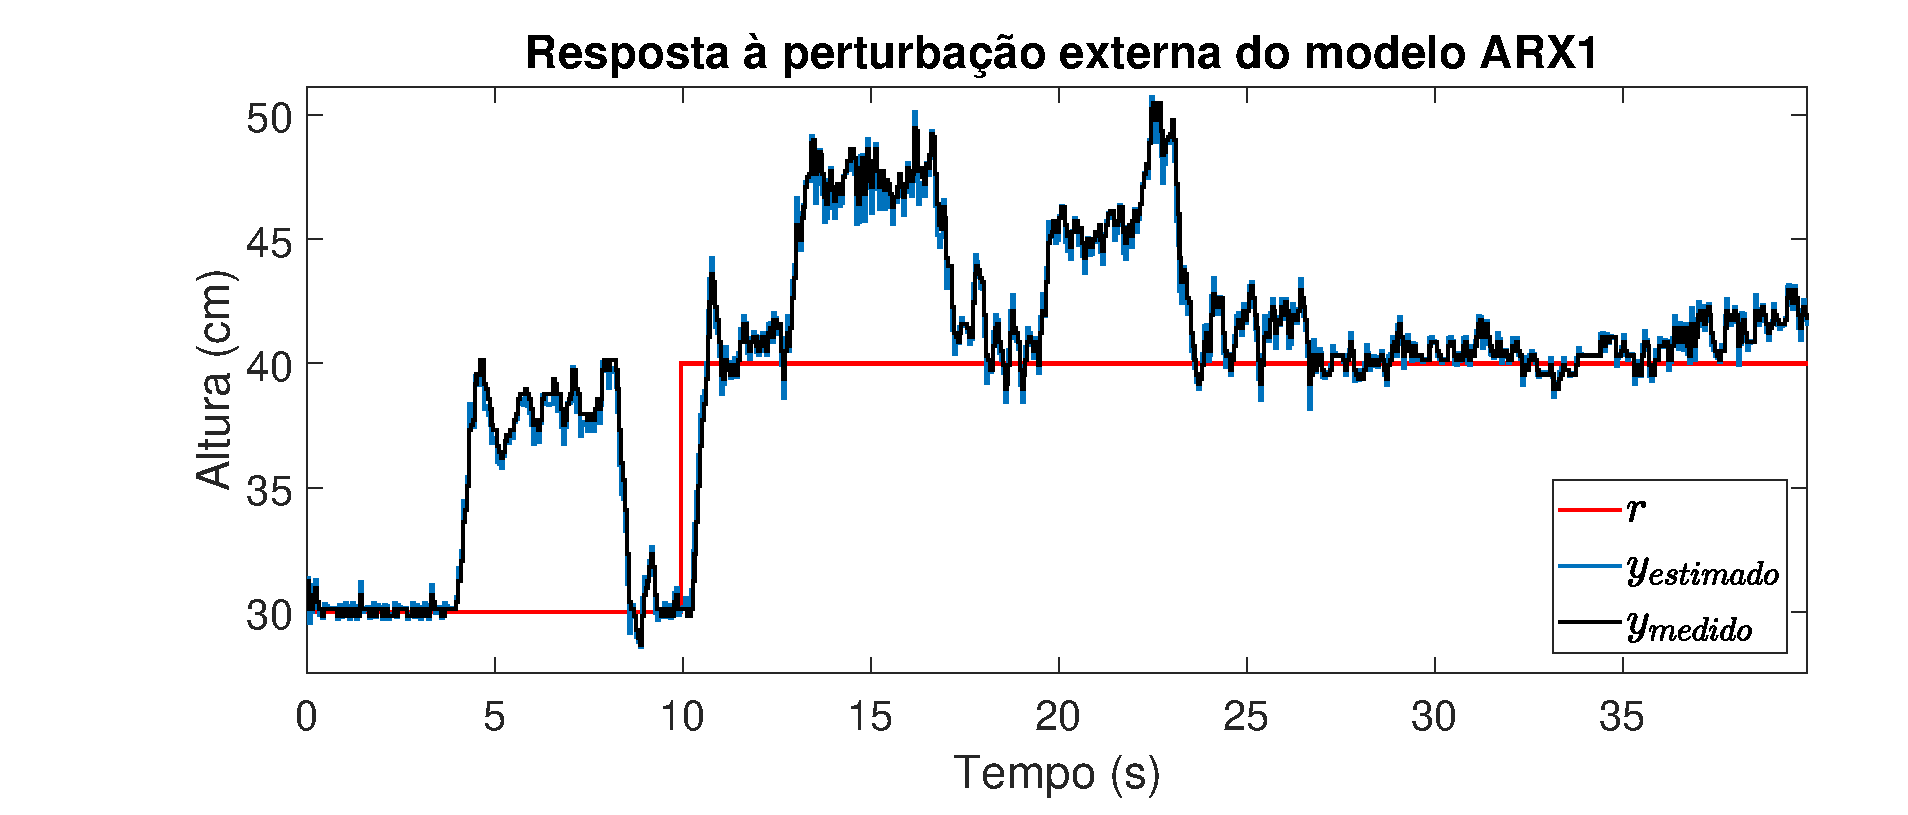
\includegraphics[width=1\linewidth]{pextrarx1y}
		\caption[$y_{estimado}$ e $y_{medido}$ do modelo $ARX1$]{$y_{estimado}$ e $y_{medido}$ do modelo $ARX1$}
		\label{fig:pextrarx1y}
	\end{subfigure}
	~ %add desired spacing between images, e. g. ~, \quad, \qquad, \hfill etc. 
	%(or a blank line to force the subfigure onto a new line)
	\begin{subfigure}[t]{0.48\textwidth}
		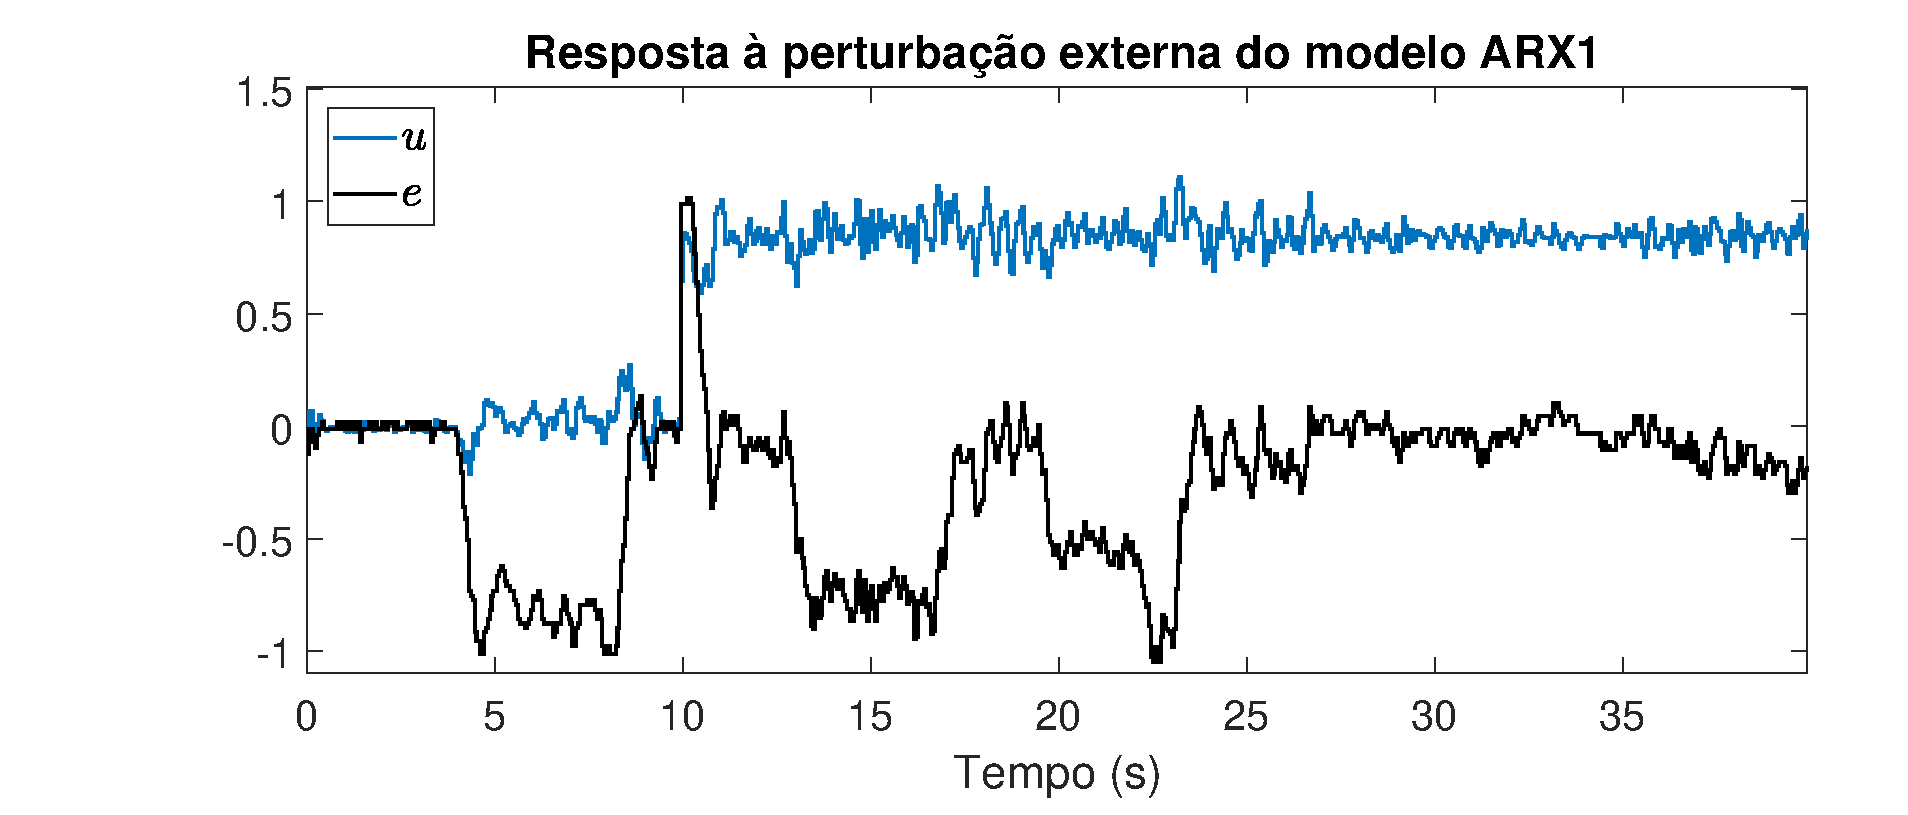
\includegraphics[width=1\linewidth]{pextrarx1e}
		\caption[erro $e$ e sinal de controle $u$ do controlador $SUB1$]{erro $e$ e sinal de controle $u$ do controlador $SUB1$}
		\label{fig:pextrarx1e}
	\end{subfigure}
	~ %add desired spacing between images, e. g. ~, \quad, \qquad, \hfill etc. 
	%(or a blank line to force the subfigure onto a new line)
	
	\caption{Resposta à perturbação externa do sistema com o controlador do modelo $ARX1$}\label{fig:pextrarx1}
\end{figure}

A resposta à perturbação externa apresentou um resultado curioso. É do nosso entendimento que um controlador seja capaz de corrigir para medidas de erro e reduzir o erro a zero. Entretanto, isso não aconteceu quando o controlador foi aplicado no sistema. Investigamos isso fazendo um teste simulado com o modelo $ARX1$ e obtivemos a figura \ref{fig:steparx1}. Com essa simulação, confirmamos que a implementação de nosso controlador não foi defeituosa, apesar de o controlador, de fato, não ter sido capaz de rejeitar perturbação externa.

\begin{figure}[htb]
	\centering
	\begin{subfigure}[t]{0.48\textwidth}
		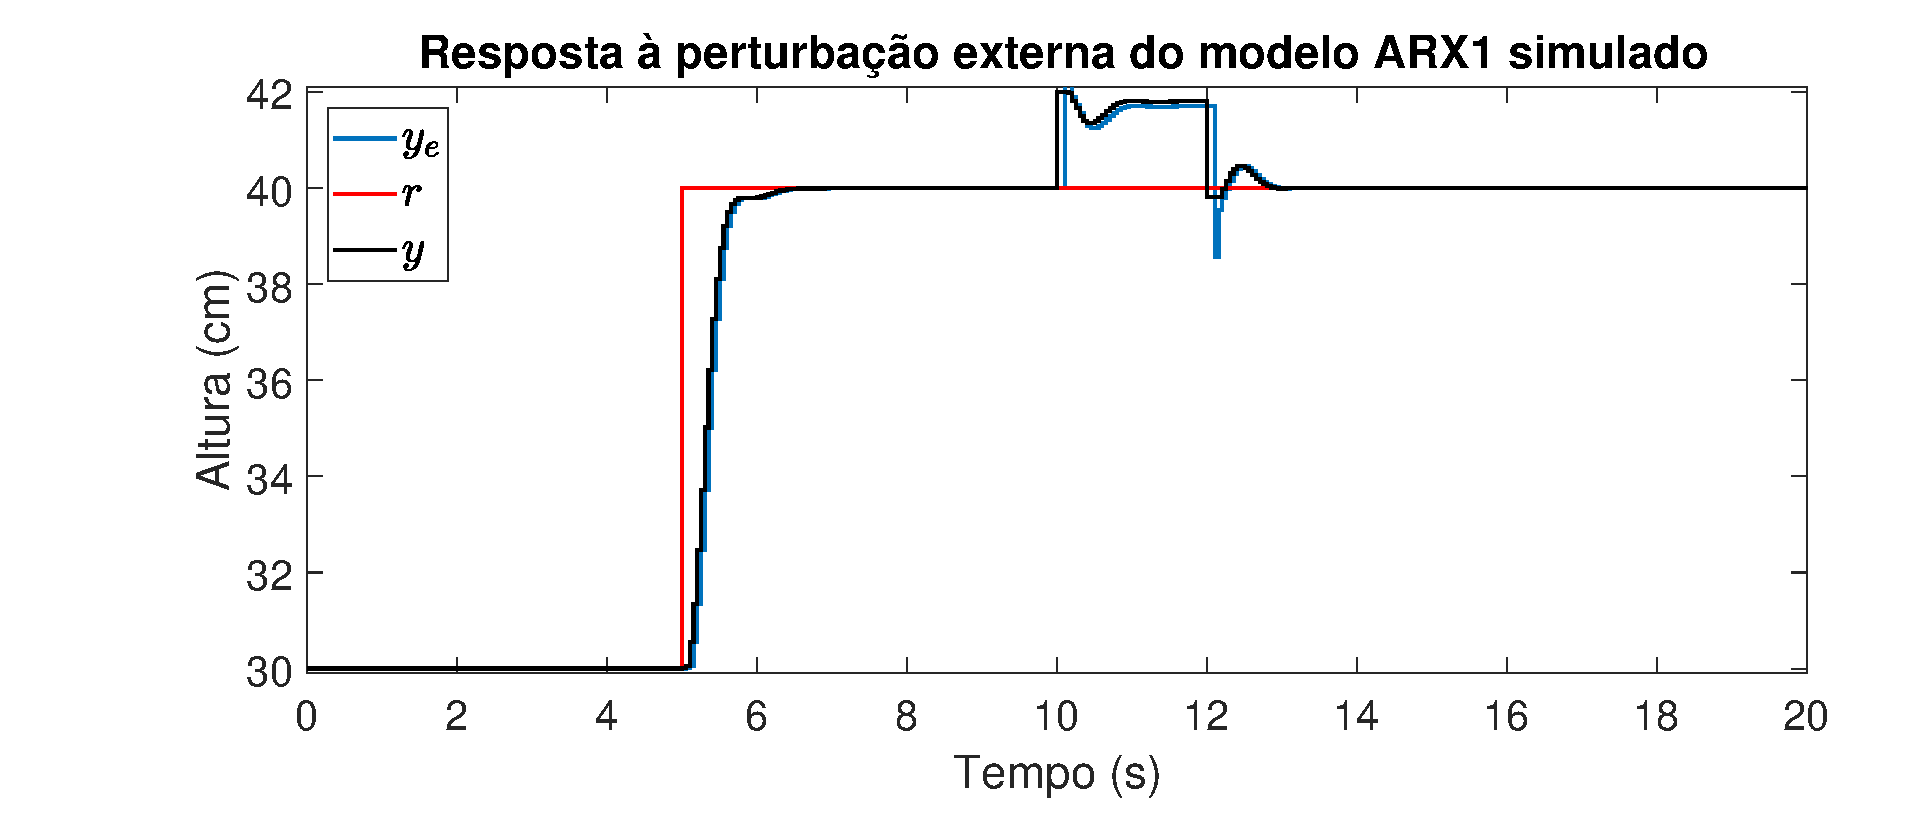
\includegraphics[width=1\linewidth]{pasta1_figuras/steparx1simy}
		\caption[$y_{estimado}$ e $y_{medido}$ do modelo $ARX1$]{$y_{estimado}$ e $y_{medido}$ do modelo $ARX1$}
		\label{fig:steparx1simy}
	\end{subfigure}
	~ %add desired spacing between images, e. g. ~, \quad, \qquad, \hfill etc. 
	%(or a blank line to force the subfigure onto a new line)
	\begin{subfigure}[t]{0.48\textwidth}
		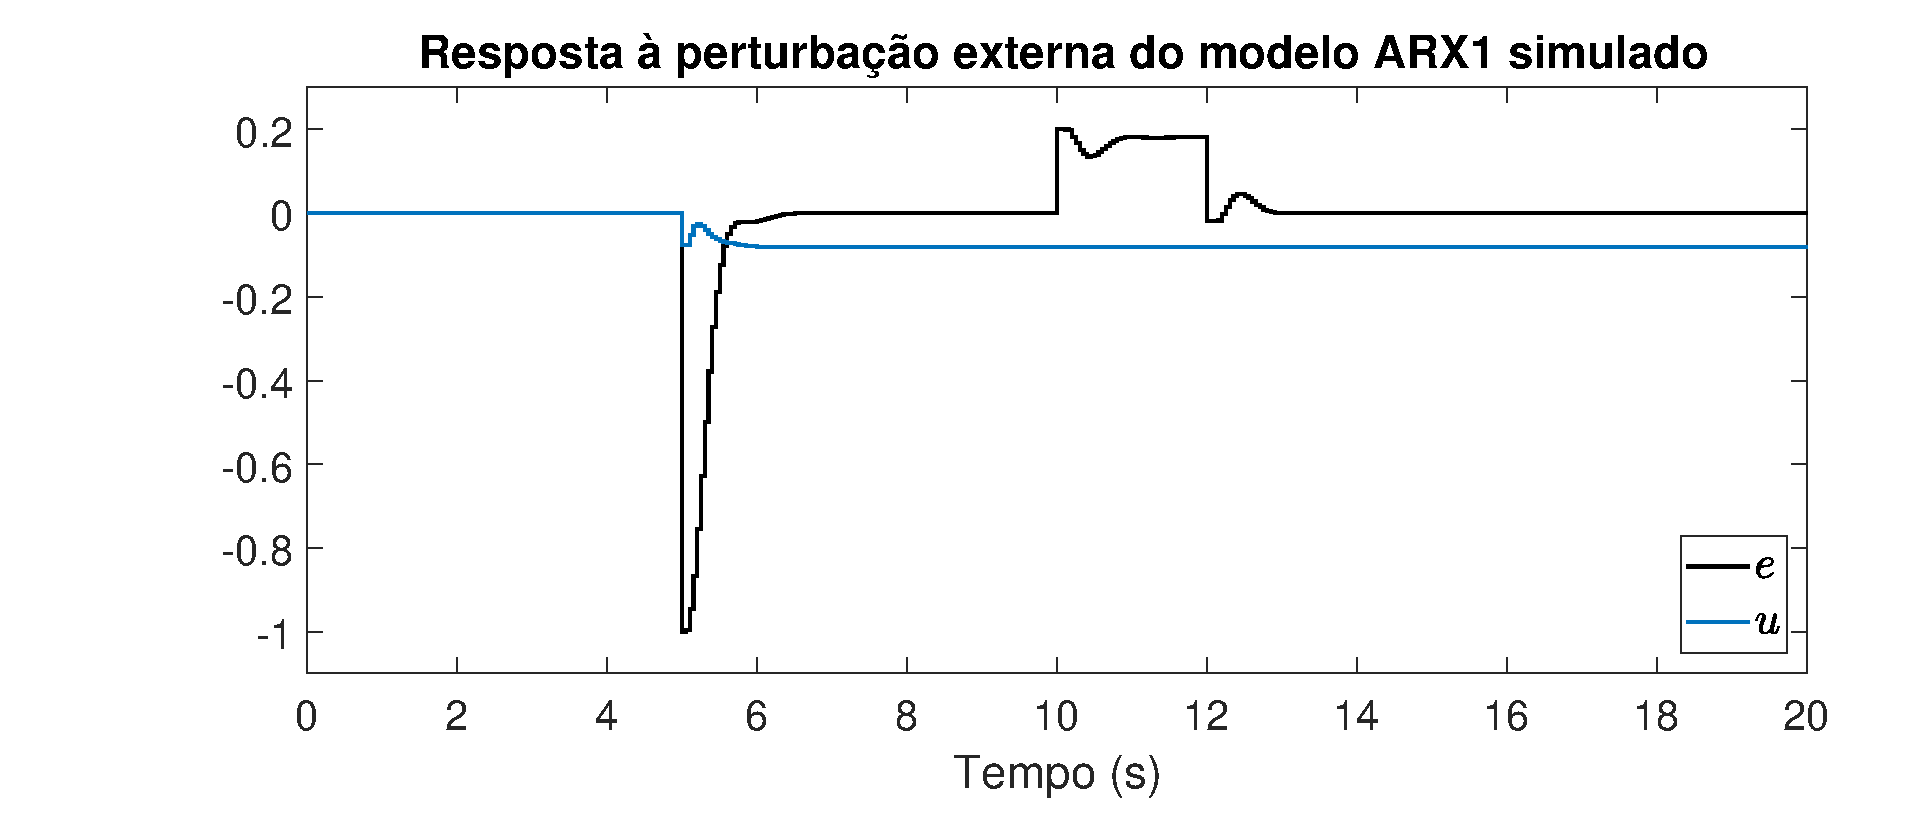
\includegraphics[width=1\linewidth]{pasta1_figuras/steparx1sime}
		\caption[erro $e$ e sinal de controle $u$ do controlador $SUB1$]{erro $e$ e sinal de controle $u$ do controlador $SUB1$}
		\label{fig:steparx1e}
	\end{subfigure}
	~ %add desired spacing between images, e. g. ~, \quad, \qquad, \hfill etc. 
	%(or a blank line to force the subfigure onto a new line)
	
	\caption{Resposta à perturbação externa do sistema com o controlador do modelo $ARX1$ simulado}\label{fig:steparx1}
\end{figure}



\subsubsection{Modelo $ARX2$}
O modelo $ARX2$ também não conseguiu seguir a referência com o aumento da bola (figura \ref{fig:pextrarx2y}).
\begin{figure}[htb]
	\centering
	\begin{subfigure}[t]{0.48\textwidth}
		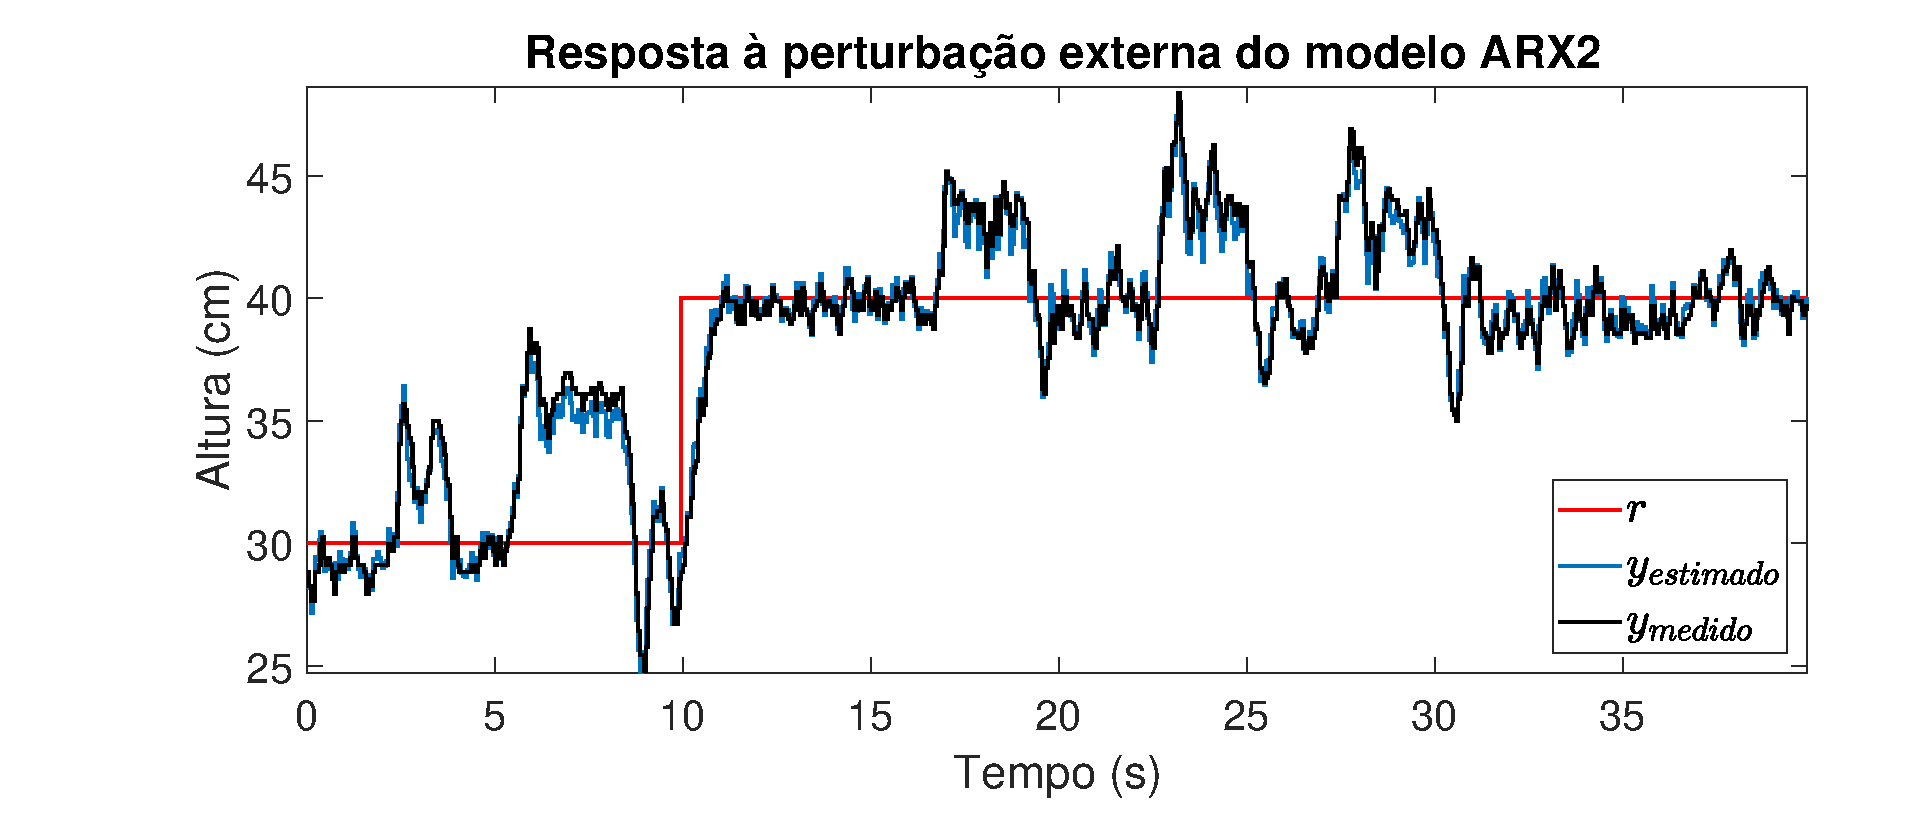
\includegraphics[width=1\linewidth]{pextrarx2y}
		\caption[$y_{estimado}$ e $y_{medido}$ do modelo $ARX2$]{$y_{estimado}$ e $y_{medido}$ do modelo $ARX2$}
		\label{fig:pextrarx2y}
	\end{subfigure}
	~ %add desired spacing between images, e. g. ~, \quad, \qquad, \hfill etc. 
	%(or a blank line to force the subfigure onto a new line)
	\begin{subfigure}[t]{0.48\textwidth}
		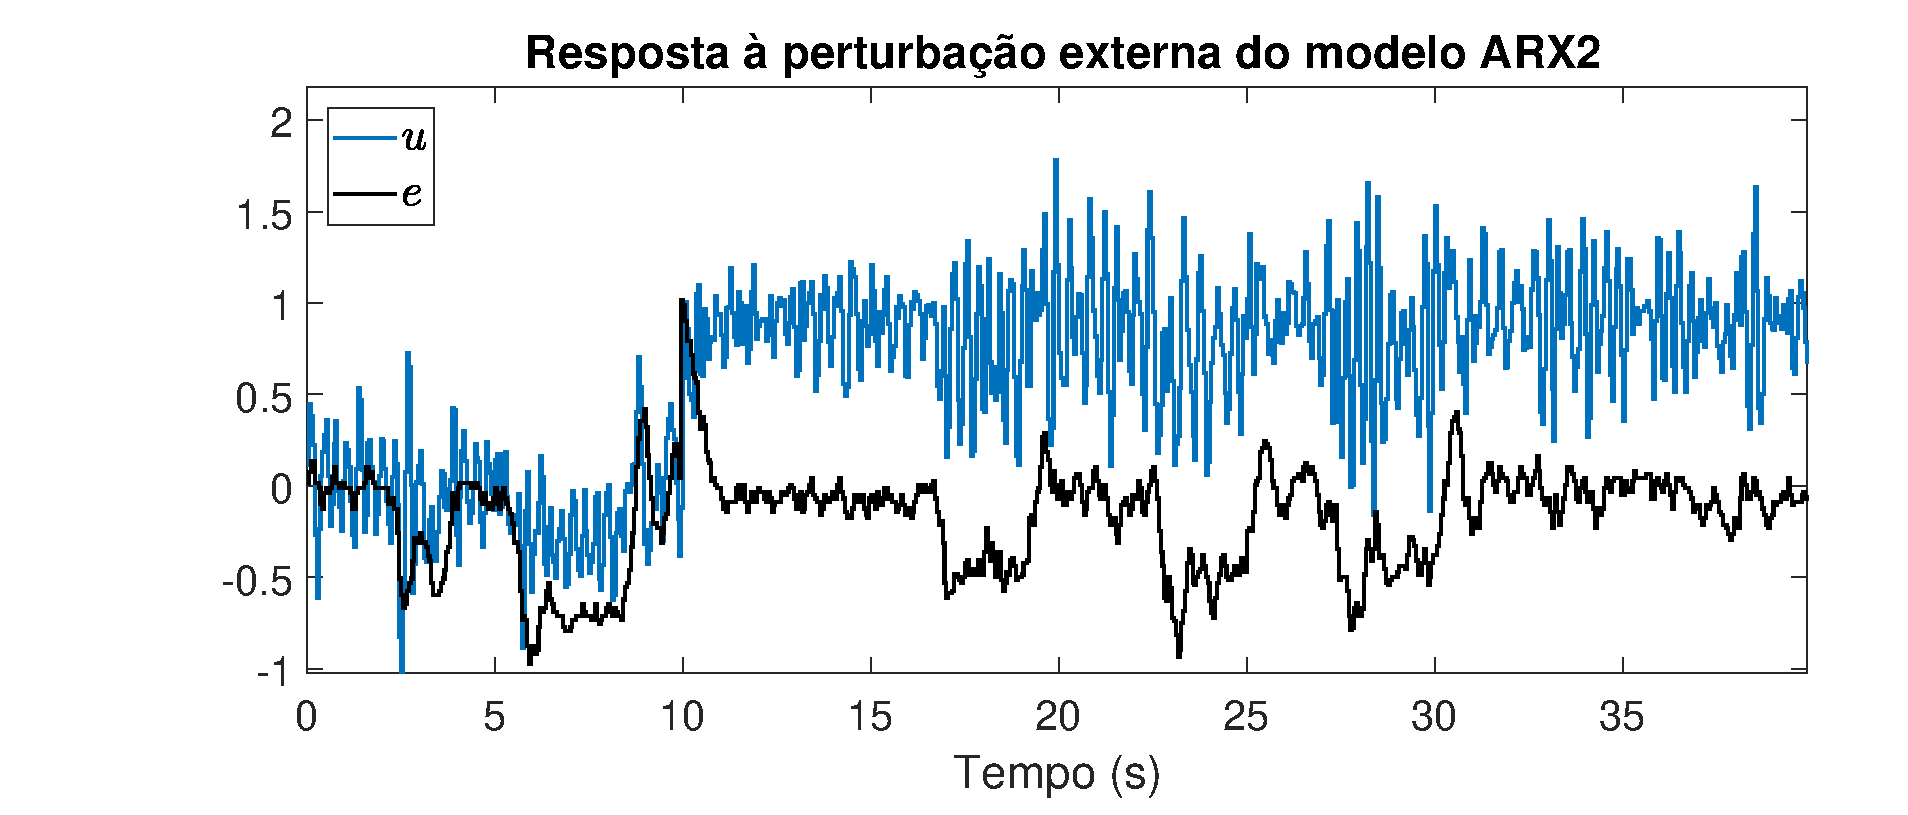
\includegraphics[width=1\linewidth]{pextrarx2e}
		\caption[erro $e$ e sinal de controle $u$ do controlador $SUB1$]{erro $e$ e sinal de controle $u$ do controlador $SUB1$}
		\label{fig:pextrarx2e}
	\end{subfigure}
	~ %add desired spacing between images, e. g. ~, \quad, \qquad, \hfill etc. 
	%(or a blank line to force the subfigure onto a new line)
	
	\caption{Resposta à perturbação externa do sistema com o controlador do modelo $ARX2$}\label{fig:pextrarx2}
\end{figure}

\subsubsection{Modelo $ARXsim$}

Testamos a resposta do modelo $ARXsim$ para perturbações externas. Vemos na figura \ref{fig:pextsarxsimy}, que o sistema não compensou para perturbações externas.

\begin{figure}[htb]
	\centering
	\begin{subfigure}[t]{0.48\textwidth}
		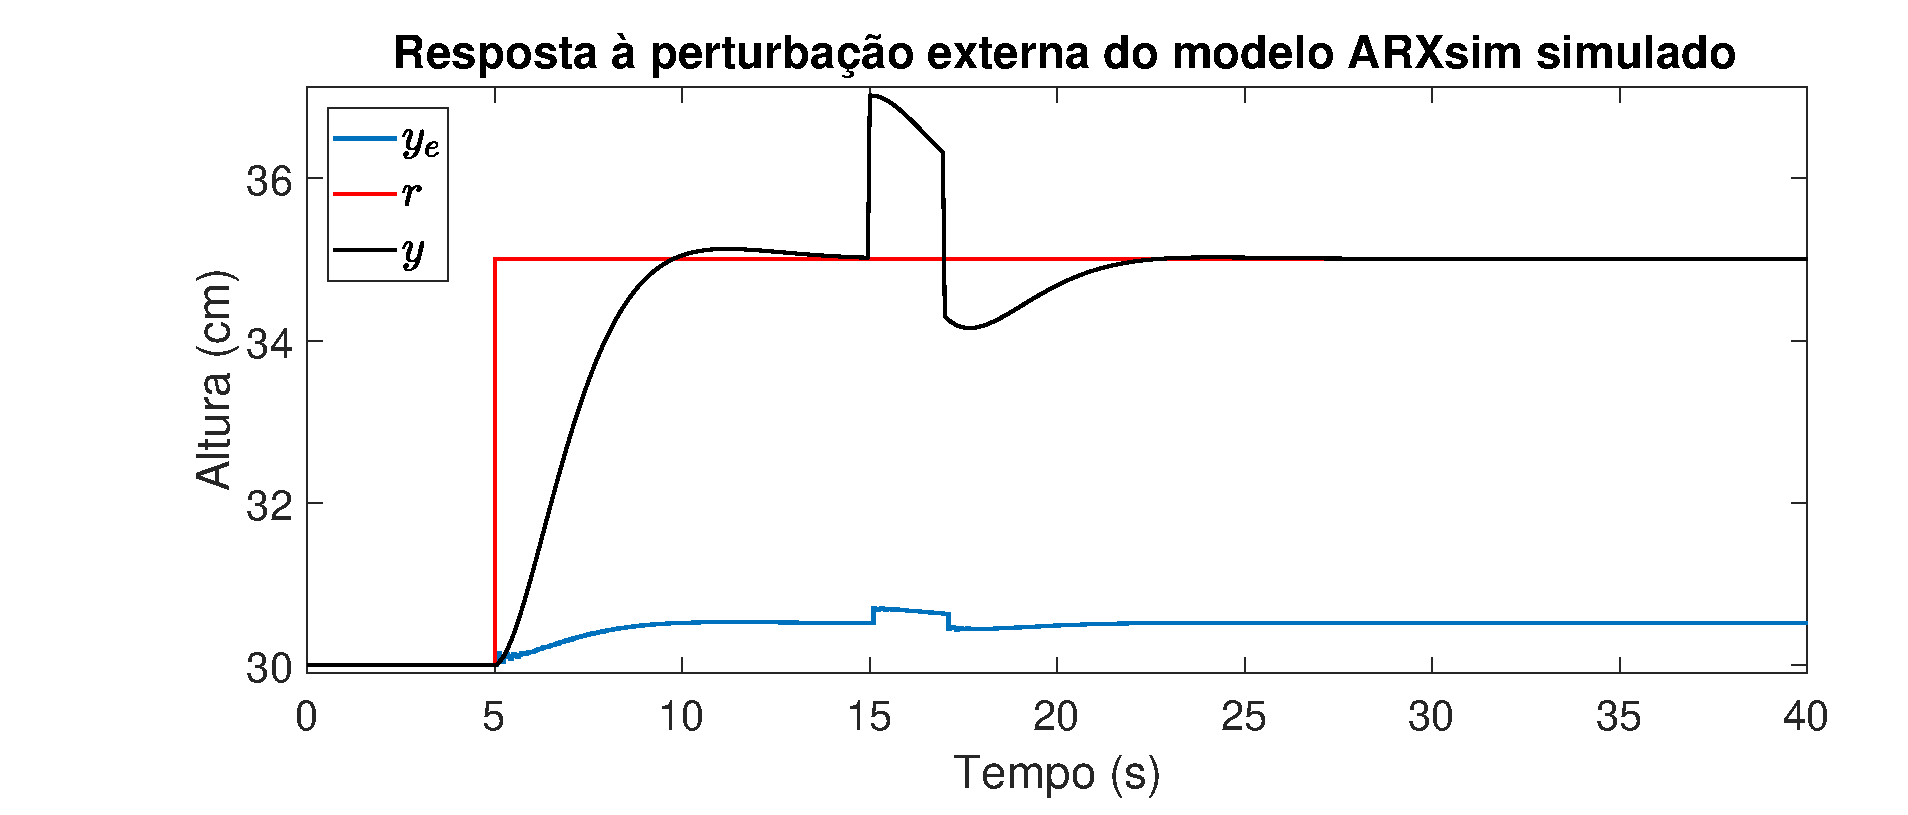
\includegraphics[width=1\linewidth]{pasta1_figuras/pextsarxsimy}
		\caption[$y_{estimado}$ e $y_{medido}$ do modelo $ARX2$]{$y_{estimado}$ e $y_{medido}$ do modelo $ARXsim$}
		\label{fig:pextsarxsimy}
	\end{subfigure}
	~ %add desired spacing between images, e. g. ~, \quad, \qquad, \hfill etc. 
	%(or a blank line to force the subfigure onto a new line)
	\begin{subfigure}[t]{0.48\textwidth}
		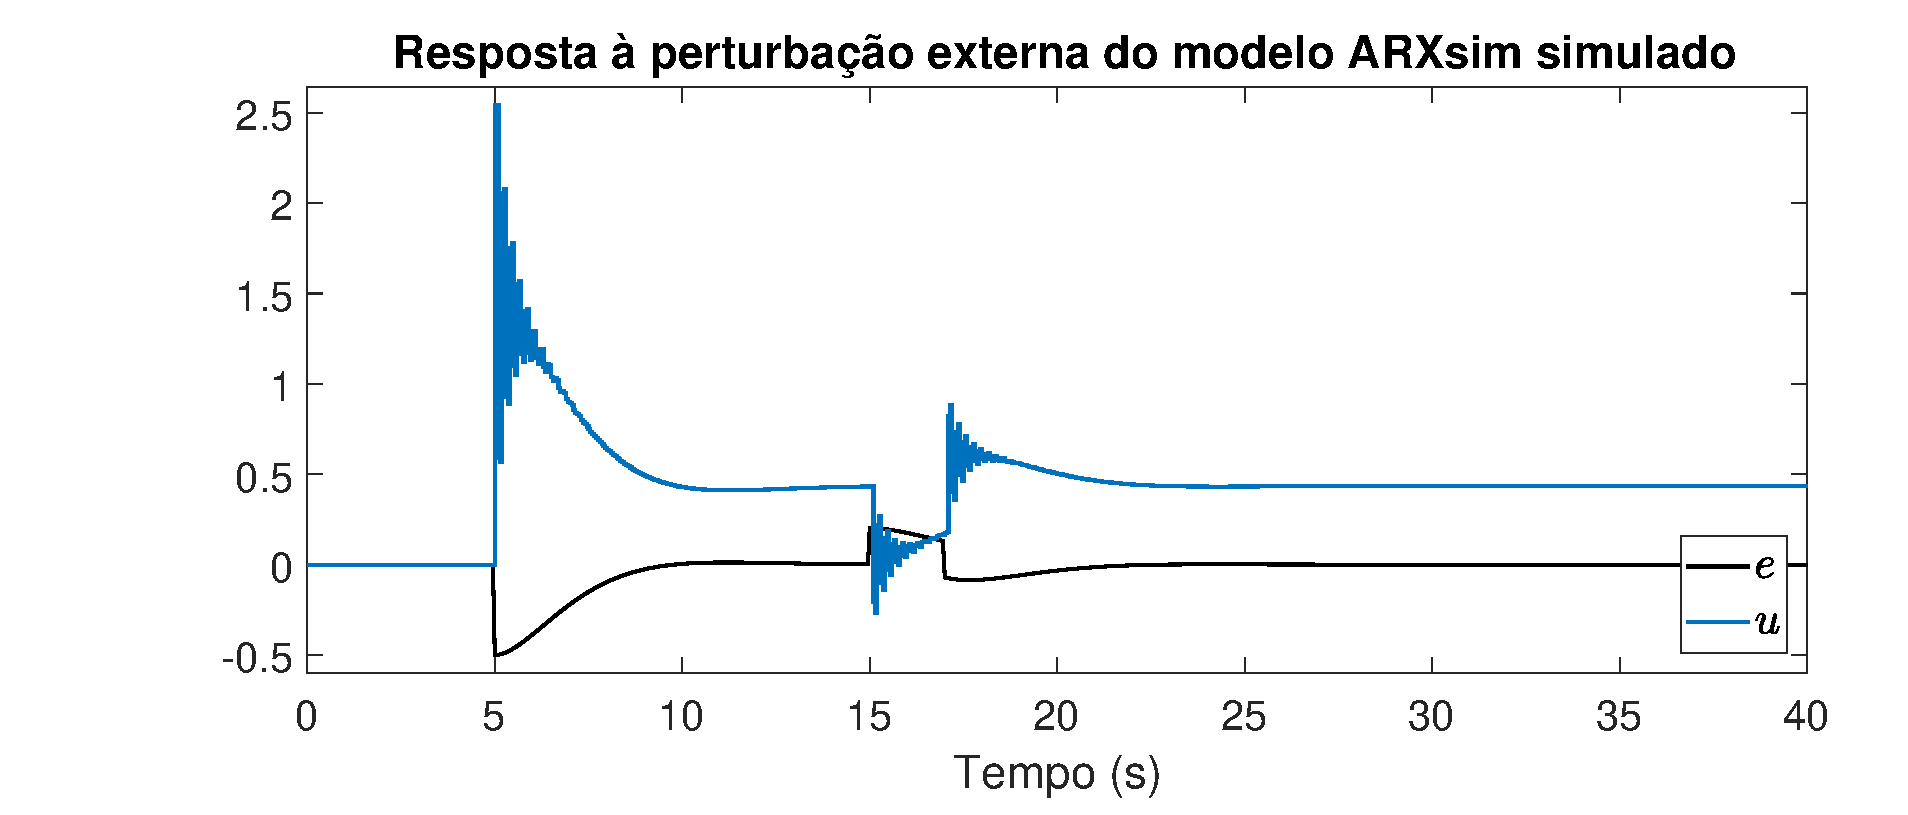
\includegraphics[width=1\linewidth]{pasta1_figuras/pextsarxsime}
		\caption[erro $e$ e sinal de controle $u$ do controlador $ARX2$]{erro $e$ e sinal de controle $u$ do controlador $ARXsim$}
		\label{fig:pextsarxsime}
	\end{subfigure}
	~ %add desired spacing between images, e. g. ~, \quad, \qquad, \hfill etc. 
	%(or a blank line to force the subfigure onto a new line)
	
	\caption{Resposta à perturbação externa do sistema com o controlador do modelo $ARXsim$}\label{fig:pextsarxsim}
\end{figure}




\section{Discussão}

Ao analisar as respostas obtidas dos experimentos, devemos levar em conta o quão ruidoso é o sensor. Apesar de aplicar um filtro na saída, ele ainda produziu valores que apresentam um alto erro de medida que, em conjunto com o giro da bola devido a força do vento, fizeram com que a leitura do sensor tivesse erros que influenciaram nos resultados.


Na seção \ref{s4:val}, mostramos que os 3 modelos, $SUB1$, $ARX1$ e $ARX2$, identificados a partir do sistema real, eram adequados para representar o sistema. O modelo $ARXsim$ identificado a partir do simulador, que continha dados experimentais do sistema sobre a velocidade do vento para diferentes PWM aplicados no motor, não apresentava as características do sistema, o que ficou evidente comparando as figuras \ref{fig:sinalprbsid} e \ref{fig:sinalprbsidsimul} que mostram as diferenças entre as respostas ao sinal PRBS. A resposta do $ARXsim$ (figura \ref{fig:respostadegrauarxsim}), foi discrepante da observada no sistema real e da observada nos outros modelos obtidos.


Essa diferença nos mostra a necessidade da identificação de um sistema usando métodos caixa-preta. Apesar de termos conseguido modelar o sistema de forma matematicamente sólida, o desempenho do modelo obtido foi divergente do sistema real. Enquanto que os modelos obtidos utilizando métodos de identificação caixa-preta conseguiram gerar modelos satisfatórios do sistema. 


Na seção \ref{s:ctrl}, projetamos um controlador por realimentação de estados, para cada um dos modelos obtidos, capaz de atender as especificações de tempo de assentamento e máximo sobrevalor definidas. Mas, devido à necessidade de criar um observador de estados na seção \ref{s5:est}, vimos que a forma como o sistema modelado atende aos requisitos mudou, mesmo se mantendo dentro dos requisitos definidos. No entanto, ao aplicar esse controlador no sistema, vimos que a resposta não estava atendendo aos requisitos estabelecidos. Projetamos ainda um controlador para o modelo obtido do simulador, identificado por caixa-cinza e, ao aplicarmos no sistema real, a resposta foi instável, reforçando a necessidade de obter modelos por identificação caixa-preta.


É interessante notar como a análise de resíduos foi uma medida capaz de prever o quão adequado um sistema é, de acordo com os dados utilizados para gerá-lo. A autocorrelação vista nas figuras \ref{fig:autocorrelacaoARX1} e \ref{fig:autocorrelacaosub1}, mostra uma grande diferença entre os sistemas, apesar de a resposta ao degrau dos modelos ser similar. O controle projetado para os modelos referidos, $ARX1$ e $SUB1$, mostra que, para que o controle seja bem sucedido, o modelo extraído tem que ser o mais fiel possível ao sistema.








